\documentclass{scrartcl}[12pt, halfparskip]
\usepackage[utf8x]{inputenc}
\usepackage[T1]{fontenc}
\usepackage[english]{babel}
\usepackage{amsmath, amssymb, amstext}
\usepackage{wrapfig}
\usepackage{float}
\usepackage{graphicx}
\usepackage{color}
\usepackage{booktabs}
\usepackage{xfrac}
%\usepackage{amsthm}
\usepackage{ntheorem}
\usepackage{subcaption}
\usepackage{bbm}
\usepackage{pdflscape}
\usepackage[linesnumbered,ruled,resetcount,algosection]{algorithm2e}
\usepackage{verbatim}


% Dies muss dringend(!) vor usepackage{varioref,hyperref,cleveref},
% sonst gibt es einen bug mit den hyperlinks wenn man draufklickt.
\numberwithin{equation}{section}
\numberwithin{figure}{section}
\numberwithin{table}{section}
%\numberwithin{algorithm}{section}


\usepackage{varioref}
\usepackage[hidelinks]{hyperref}
\usepackage{cleveref}


%\theoremstyle{break}
\newtheorem{Definition}{Definition}
\newtheorem{Theorem}{Theorem}
\newtheorem{Lemma}{Lemma}



\usepackage{pgfplots}
\usepackage{tikz}
\usetikzlibrary{fit} 
\usetikzlibrary{external}
%\tikzexternalize % activate!
%\usetikzlibrary{patterns}
\usetikzlibrary{patterns,decorations.pathreplacing}


    \tikzset{
    	hatch distance/.store in=\hatchdistance,
    	hatch distance=10pt,
    	hatch thickness/.store in=\hatchthickness,
    	hatch thickness=2pt
    }
    
    \makeatletter
    \pgfdeclarepatternformonly[\hatchdistance,\hatchthickness]{flexible hatch}
    {\pgfqpoint{0pt}{0pt}}
    {\pgfqpoint{\hatchdistance}{\hatchdistance}}
    {\pgfpoint{\hatchdistance-1pt}{\hatchdistance-1pt}}%
    {
    	\pgfsetcolor{\tikz@pattern@color}
    	\pgfsetlinewidth{\hatchthickness}
    	\pgfpathmoveto{\pgfqpoint{0pt}{0pt}}
    	\pgfpathlineto{\pgfqpoint{\hatchdistance}{\hatchdistance}}
    	\pgfusepath{stroke}
    }
    \makeatother



\newcommand\raalign[2]{%Umrahmen einer align-Gl.
	\tikz[overlay,every node/.style={inner sep=-2pt,outer sep=0pt}]%
	\node[anchor=base west](g){\phantom{$\displaystyle #1\null=\null#2$}}%
	node[draw=blue!50!black,fill=white!10,fit=(g),inner sep=5pt]{};%
	#1#2}


\usepackage{empheq}
\newcommand*\widefbox[1]{\fbox{\hspace{2em}#1\hspace{2em}}}


\usepackage{caption}
\usepackage{subcaption}

\bibliographystyle{unsrt}

\setlength{\parindent}{0pt}

\newcommand{\todo}[1]{\textcolor{red}{TODO: #1}}
\newcommand{\bem}[1]{\textcolor{blue}{Bem.: #1}}

\newcommand{\var}{\operatorname{Var}}

\newcommand\undermat[2]{% http://tex.stackexchange.com/a/102468/5764
	\makebox[0pt][l]{$\smash{\underbrace{\phantom{%
					\begin{matrix}#2\end{matrix}}}_{\text{$#1$}}}$}#2}

\title{Master Thesis}


\author{Jan Lammel}
\date{\today{}, Heidelberg}



\begin{document}

 \pagenumbering{Roman}  

%\begin{titlepage}
%	\begin{center}
%	
%	\textsc{\large Ruprecht-Karls-Universit\"{a}t Heidelberg} \\[0.5cm]
%	\textsc{\large Master Thesis}\\[0.5ex]
%	\textsc{\large in the field of study}\\[0.5ex]
%	\textsc{\large Scientific Computing}\\[1cm]
%	
%	\newcommand{\HRule}{\rule{\linewidth}{0.5mm}}
%	\HRule \\[0.4cm]
%	\huge \bfseries Simulation of heat flux differential scanning calorimetry with phase change materials and parameter estimation of the specific heat capacity 
%	\HRule 
%	
%	\vspace{6.5cm}
%	
%	\Large \textit{Jan Lammel} \\
%	\Large \textit{born in Heidelberg} \\[4ex]
%	\Large \textit{Heidelberg, \today }\\[3ex]
%	\Large \textit{Supervisor:}\\
%	\Large \textit{Prof. Dr. Dr. h. c. mult. Hans Georg Bock}\\
%	\Large \textit{\todo{...}}
%	
%	\end{center}
%\end{titlepage}



\begin{titlepage}
	\begin{center}
		
	\Large{Department of Mathematics and Computer Science} \\[3ex]
	
	University of Heidelberg \\
	
	\vspace{13cm}
	
	Master Thesis \\[0.5ex]
	in Scientific Computing \\[2ex]
	submitted by \\[2ex]
	Jan Lammel \\[0.5ex]
	born in Heidelberg \\[3ex]
	2018 \\[2ex]
		
	\end{center}
\end{titlepage}


\newpage 

\begin{titlepage}
	\mbox{}\\
\end{titlepage}

\begin{titlepage}
	\begin{center}
		\newcommand{\HRule}{\rule{\linewidth}{0.5mm}}
		\HRule \\[0.1cm]
%		{\huge \bfseries Simulation of heat flux differential \\[0.1ex]
%		scanning calorimetry with phase change \\[0.1ex]
%		materials and parameter estimation of the \\[0.2ex]
%		specific heat capacity }
		{\huge \bfseries Heat flux differential scanning calorimetry simulation and applied parameter estimation of the specific heat capacity of phase change materials}
		\HRule \\[0.3cm]
		
		\vspace{10cm}
		
		{\Large This master thesis has been carried out by Jan Lammel \\[2ex]
		at the \\[2ex]
		Interdisciplinary Center for Scientific Computing (IWR)\\ 
		in the group Simulation and Optimization \\[3ex]
		under the supervision of \\[3ex]
		Herrn Prof. Dr. Dr. h. c. mult. Hans Georg Bock}
	\end{center}
\end{titlepage}

\newpage


\begin{titlepage}
	\mbox{}\\
\end{titlepage}



\section*{Abstract}

This thesis approaches the problem of identifying the specific heat capacity $c_p$ of phase change materials (PCM). An usual method using measurement data of heat flux differential scanning calorimetry (DSC) results in different outcomes dependent on a measurement parameter, the heat rate. 
Therefore in this thesis a new developed model is introduced to simulate the measuring process of a heat flux DSC where phase change materials are used as sample. 
The simulation is accomplished by solving the heat equation where the PCM's specific heat capacity is temperature dependent and has a phase transition peak. 
This simulation is capable of reproducing heat fluxes into the sample analogously to the physical experiment. 
With this insight the simulation has been embedded in a least squares parameter estimation framework using heat flux measurement data in order to estimate the sample's specific heat capacity, independently from the heat rate. With $c_p(T)$ parametrized with a Fraser-Suzuki peak and linear baseline, a distinct reduction in the deviation of peak characteristics maximum position $T_{max}$, offset of melting $T_{off}$ and melting enthalpy $\Delta H$ for specified heat rates was possible.



\section*{Kurzbeschreibung}

\todo{!}

\newpage



\tableofcontents 
\newpage


\pagenumbering{arabic}
\addsec{Summary}
This thesis comprises the modeling of and parameter estimation in the physical measurement process of heat flux differential scanning calorimetry (DSC). As part of the research project modELTES, phase change materials (PCM) are analyzed with respect to their specific heat capacity $c_p$. Therefore a new model of the measuring process of a heat flux DSC has been developed. This model is embedded in a parameter estimation framework to identify the PCM's specific heat capacity. \\

The thesis begins with a general introduction in \cref{sec:introduction} about PCMs with exemplary applications of those and the motivation of developing a new method for the identification of the specific heat capacity. \Cref{sec:physical_background} introduces the physical quantities, relevant for further comprehension. The physics of a phase transition is elucidated including its relation to the temperature dependent specific heat capacity, exhibiting a phase transition peak.
Associated characteristic quantities, namely maximum position $T_{max}$, on- and offset of melting $T_{on}$ and $T_{off}$, respectively and melting enthalpy $\Delta H$ are explained further. The heat equation, essential for our mathematical model, is derived. The physical measurement process of differential scanning calorimetry (DSC) is elucidated, origin of the measurement data deployed later in the parameter estimation. \Cref{sec:physical_background} concludes with expounding the smearing problem, occurring for a hitherto usual way of computing $c_p(T)$ from DSC measurement data. The obtained $c_p(T)$ here depend on the heat rate, a measurement parameter. Since $c_p(T)$ is a material property, this is unphysical and further, a motivation of this thesis to avoid this problem in a parameter estimation framework. \\ 
Mathematical problems within the scope of this thesis and corresponding methods for their (numerical) solution are elucidated in \cref{sec:mathematical_background}. Two approaches of generating derivatives are shown. First, in an approximative way by finite differences and secondly via Automatic Differentiation (AD). In this context, variational differential equations are explained regarding the sensitivities of a differential equation w.r.t. its parameters. The used methods of obtaining these sensitivities by applying internal numerical differentiation (IND) and AD is shown. An essential problem is the initial value problem (IVP). Its numerical solution via the backward differentiation formula (BDF) method is presented. As the heat equation occurs in the model, the method of lines for a spatial discretization of parabolic partial differential equations (PDE) is introduced and applied on an analogous boundary value problem (BVP) as in our model. Fundamentals on optimization theory and especially regarding nonlinear least squares problems are depicted. In this context, the Gauss-Newton method is presented inclusively aspects on the numerical implementation. The parameter estimation problem with least squares objective is formulated and discussed with respect to confidence regions of the obtained parameters in an a posteriori analysis. \\
\Cref{sec:simulation_of_DSC} introduces the new model to simulate the measuring process of heat flux DSC. In this model the heat equation occurs which is treated with the mathematical methods introduced, resulting in an IVP to solve. The construction of the spatial discretization grid is presented, which occurs in the context of the method of lines. In one part of the model, the diffusion constant of the heat equation is constant. Therefore, the corresponding analytical solution of this subproblem is derived. The least squares optimization problem for the parameter estimation is formulated in \cref{sec:parameter_estimation_applied}. In this context, the three parametrizations of $c_p(T)$ used in the scope of this thesis are introduced. Namely these are NURBS, a linear combination of Gaussians and a Fraser-Suzuki peak. The measurement times are not given but needed in the optimization problem. Therefore, these are computed via the derived analytical solution of the heat equation. In order to apply the Gauss-Newton method to solve the nonlinear least squares problem, the residuum function is defined and corresponding Jacobian is derived. \\
The conducted numerical experiments are presented and evaluated in \cref{sec:numerical_experiments}. First, the capability of the new model to reproduce heat fluxes similar to those measured is shown. In a preliminary study the optimization is performed with NURBS parametrization and the Jacobian of the objective function is computed by finite differences. The occurred problems with this setting are analyzed. An error analysis with respect to the integration accuracy is performed in order to assess its influence on the results. With analogous intention, the spatial discretization grid has been varied and compared with an equidistant grid. The parameter estimation with the parametrization of linear combination of Gaussians is examined. Here and in the following, exact numerical sensitivities computed via IND and AD are used. The specific heat capacity, estimated for each heat rate separately, is analyzed. An a posteriori analysis of the obtained parameters is performed, showing indications of overfitting. A collective comparison of $c_p(T)$, obtained by the different heat rates, and its peak characteristics is conducted. The parameter estimation with Fraser-Suzuki parametrization is performed and analyzed analogously. Additionally, the Gauss-Newton iterates in the optimization process are examined and compared to theoretical expectations. Due to the observation of a small deviation of the nominal and measured heat rate in the experiment, the parameter estimation is performed again with the mean value of the measured heat rate. No significant difference to the results before is observed here, indicating a small sensitivity with respect to the heat rate. \Cref{sec:numerical_experiments} concludes with a comparison of $c_p(T)$ obtained both by an hitherto usual method and the parameter estimation performed in this thesis. This leads to the result that the deviation of the peak characteristics $T_{max}$, $T_{off}$ and $\Delta H$ among the different heat rates is reduced significantly with the parameter estimation with Fraser-Suzuki parametrization. \\
The thesis concludes in \cref{sec:discussion} with a discussion of the results, occured problems and possibilities for future work on this subject.


\newpage


\section{Introduction}
\label{sec:introduction}
This thesis is part of project modELTES, a cooperation of the Austrian Institute of Technology GmbH (AIT), VOIGT+WIPP Engineers GmbH and Interdisziplinäres Zentrum für Wissenschaftliches Rechnen (IWR) here at Ruprecht-Karls-Universität Heidelberg in order to examine so called phase change materials (PCM). The physical experiments have been performed in Wien at the AIT while in Heidelberg the aim is on the development of simulation software. \\
A popular application of PCMs are heating pads (see \cref{fig:heating_pad}) which are liquid in fully charged state. Folding induces a phase change to a solid state where energy is released and therefore the temperature increases. They can be recharged by applying a temperature for a sufficiently long time above the melting point (e.g. with boiling water). 

\begin{wrapfigure}{l}{0.4\textwidth}
	\includegraphics[width=0.4\textwidth]{/home/argo/masterarbeit/thesis/images/handwaermer[wiki].jpg}
	\caption{Heating pad \\ left: liquid; right: solid \\
		Source: \cite{heating_pad_image}}
	\label{fig:heating_pad}
\end{wrapfigure}

%\begin{figure}[H]
%	\centering
%	\includegraphics[width=0.6\textwidth]{/home/argo/masterarbeit/thesis/images/handwaermer[wiki].jpg}
%	\caption{Heating pad, left: liquid; right: solid, Source: \cite{heating_pad_image}}
%	\label{fig:heating_pad}
%\end{figure}

In general, PCMs work as an energy buffer. Another application are industry processes to store the process heat for later usage \cite{pcm_process_heat}. Furthermore they can be used to optimize  photovoltaic cells as the efficiency of those cells is temperature dependent with a maximum at a certain point. PCMs are able to stabilize the temperature where the efficiency is maximal \cite{pcm_solar_cells}. 
A last example are insulations of houses. During the day when it is hot, the PCM becomes liquid and absorbs heat from outside, so they work as a cooling system. On the contrary at night when it is cold outside the PCM becomes solid, releases heat and works as a heating \cite{pcm_house_insulation}. \\
An important material property is the specific heat capacity $c_p(T)$ where a phase transition peak tells us at which temperature the phase change occurs and how much energy can be stored. The common way of computing $c_p(T)$ from differential scanning calorimetry (DSC) measurement data yields different results depending on the heat rate, a measurement parameter. Since $c_p(T)$ is a material property this is unphysical and this issue is known as the smearing problem. By applying a parameter estimation we aim to avoid this problem.
Therefore the two major goals of this thesis is both simulate the measuring process of a DSC where a PCM undergoes a phase transition and perform a parameter estimation in order to get the PCM's true specific heat capacity. 
Furthermore the heat rate is proportional to the time duration of the experiment. If we get the same $c_p(T)$ for all heat rates we are able to accelerate the measuring process and therefore the research on this materials. \\
This thesis is structured as follows. In \cref{sec:physical_background} the physics of a phase transition and the measuring process of a DSC are elucidated. 
The mathematical methods for simulation and parameter estimation are introduced in \cref{sec:mathematical_background}. These methods then have been applied in \cref{sec:simulation_of_DSC} to simulate the DSC measuring process and in \cref{sec:parameter_estimation_applied} for the parameter estimation of the specific heat capacity. Performed numerical experiments and corresponding results are shown in \cref{sec:numerical_experiments}. Finally \cref{sec:discussion} concludes this thesis with a discussion of results, problems and potential next working steps on this subject.


\section{Physical background}
\label{sec:physical_background}

Since the work in this thesis is based on the experiments of a differential scanning calorimetry, the physical basics regarding important quantities, phase transition and the experimental setup will be introduced. Further, the heat equation will be derived, which is relevant for the simulation model later. Finally as motivation the smearing problem occurring in the hitherto usual method of computing the specific heat capacity is shown.


\subsection{Physical quantities and phase transition}

First of all some important physical quantities will be introduced because they are crucial for further comprehension. A summary is shown in \cref{tab:important_physical_quantities} with the consistently used symbols in this thesis and the physical unit. \\
Heat $Q$ is the energy that flows from a warmer to a colder object because of the temperature difference. The heat flux density $\phi$ tells us how much heat flows through an unit area in one second. By considering a particular area this quantity becomes the heat flux $\varPhi$. Heat conductivity $\lambda$ is a material property how much energy is transported on a distance of $1m$, unit area and temperature difference of $1K$ in one second.

\begin{table}[H]
	\centering
\begin{tabular}{| c | c | c |} \hline
	Quantity & Symbol & Unit \\ \hline
	Heat & $Q$ & $J$ \\[0.7ex]
	Heat flux density & $\phi$ & $\frac{W}{m^2}$ \\[0.7ex]
	Heat flux & $\varPhi$ & $W$ \\[0.7ex]
	Heat conductivity & $\lambda$ & $\frac{W}{m \cdot K}$ \\[0.7ex]
	Specific heat capacity & $c_p$ & $\frac{J}{kg \cdot K}$ \\[0.7ex]
	Melting enthalpy & $\Delta H$ & $J$ \\ \hline
\end{tabular}
\caption{Important physical quantities in SI units}
\label{tab:important_physical_quantities}
\end{table}



Probably the most important physical quantity for us is the specific heat capacity $c_p$, a temperature dependent material property that tells us how much energy is needed to increase the temperature of $1kg$ of this material by $1K$. 
Since we are primarily interested in the phase change we handle with specific heat capacities with latent part, i.e. a peak at the melting point. Moreover the specific heat capacity not belonging to the phase transition is called sensitive part and is described by the base line. 
For a pure substance this phase transition peak would be ideally a Dirac delta function (see  \cref{fig:physics_c_p_dirac_delta}). A constant heat flux entering such a pure substance increases the temperature until phase change. Then the heat is absorbed in order to perform the phase transition while the temperature stays constant. Finally, after the phase change has finished, the temperature increases again. 
In mixed substances like polyethylene in our case with different lengths of the individual polymer chains or due to lattice defects, the peak extends over a temperature range. In the case of lattice defects the atom's binding energies are decreased which lowers the phase transition's temperature partially. The corresponding shape of the specific heat capacity is shown in \cref{fig:physics_fraser_suzuki}. It is not known what shape of $c_p(T)$ we should expect exactly for a polymer. \\
The last physical quantity to introduce is the melting enthalpy $\Delta H$ which is in the case of constant pressure the heat needed to perform the phase transition. Considering the graph $c_p(T)$, the area below the phase change peak less the baseline is equal to the melting enthalpy. This is illustrated in \cref{fig:physics_fraser_suzuki}.



\begin{figure}[H]
\hspace{-2cm}
\begin{subfigure}{0.49\textwidth}
\begin{tikzpicture}
\begin{axis}[domain=70:150,
samples=500,
ymin=0, ymax=15	,	
xmin=70, xmax=150,	 
axis lines=left,
xtick=\empty,
ytick=\empty,
xlabel=$T$, xlabel style={at=(current axis.right of origin), anchor=west},
ylabel=\empty, ylabel style={at=(current axis.above origin), anchor=south}]

\addplot+[color=blue,
mark=none] {1.};
\addlegendentry{$c_p(T)$}

\draw[-latex,blue] (axis cs:130,1.) -- (axis cs:130,10);

\end{axis}
\end{tikzpicture}
\caption{}
\label{fig:physics_c_p_dirac_delta}
\end{subfigure}
\hspace{1.cm}
\begin{subfigure}{0.49\textwidth}
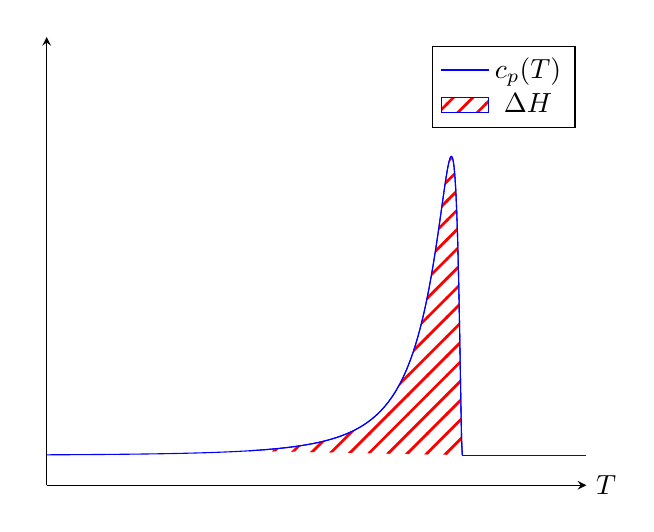
\begin{tikzpicture}
\begin{axis}[domain=70:132,
samples=500,
ymin=0, ymax=15	,	
xmin=70, xmax=150,	 
axis lines=left,
xtick=\empty,
ytick=\empty,
xlabel=$T$, xlabel style={at=(current axis.right of origin), anchor=west},
ylabel=\empty, ylabel style={at=(current axis.above origin), anchor=south}]

\addplot+[color=blue,
mark=none] {10*exp(-ln(2)/ln(0.3)^2 * (ln(1 + (x-130)*(0.3^2 - 1)/(5*0.3)))^2) + 1.};
\addlegendentry{$c_p(T)$}

\addplot+[mark=none,
color=blue,
domain=131.64:150,
samples=50,
forget plot]
{1.};

\addplot+[mark=none,
domain=100:132,
samples=500,
pattern=flexible hatch,
hatch distance=8pt,
hatch thickness=1pt,
draw=blue,
pattern color=red,
area legend]
{10*exp(-ln(2)/ln(0.3)^2 * (ln(1 + (x-130)*(0.3^2 - 1)/(5*0.3)))^2) + 1.};
\addlegendentry{$\Delta H$}
\end{axis}
\end{tikzpicture}
\caption{}
\label{fig:physics_fraser_suzuki}
\end{subfigure}
\caption{Specific heat capacity for (a) ideally pure substance where the phase transition is described by a Dirac delta function at the melting point and (b) mixed substance where melting enthalpy $\Delta H$ is illustrated.}
\end{figure}

\subsection{Phase transition peak characteristics}
\label{sec:peak_characteristics}
Beside the melting enthalpy $\Delta H$ (\cref{fig:physics_fraser_suzuki}) additional characteristics are introduced in order to quantify a given peak.


\begin{figure}[H]
	\centering
	\includegraphics[width=0.79\textwidth]{/home/argo/masterarbeit/thesis/images/T_on_T_off_illustration.png}
	\caption{Illustration of peak characteristics $T_{max}$, $T_{on}$ and $T_{off}$ where latter two are computed as intersections of the base line with inflection point tangents. \\
	Used for evaluation in numerical experiment \cref{sec:param_estimation_5Gausse,sec:param_estimation_fs,sec:param_estimation_mod_heat_rate_FS}.}
	\label{fig:T_on/off_illustration}
\end{figure}

These are the maximum point $T_{max}$ and further the extrapolated on- and offset of melting $T_{on}$ and $T_{off}$ computed as the intersection of the inflection points' tangents with the base line of $c_p(T)$, i.e. the sensitive part \cite{DIN_11357}. In the parametrizations (\cref{sec:parametrizations} except NURBS) of the specific heat capacity in this thesis the base line is modeled linear. An illustration is given above in \cref{fig:T_on/off_illustration}.


\subsection{Derivation of the heat equation}
\label{sec:heat_equation}

Since we are dealing with heat transport in the measuring process, the central physical equation in this thesis is the heat equation. \\
For its derivation \cite{lit:waerme_und_stoffuebertragung}
we start with the total inner energy $U$ in a volume $V$ which can be computed by

\begin{equation}
	U = \int_{V} \rho u \ dV
\end{equation}

where $\rho$ is the mass density and $u$ is the specific inner energy. \\
The total heat flux $\varPhi$ into the volume $V$ is

\begin{equation}
	\varPhi = - \int_{\partial V} \phi \cdot n \ dA = - \int_{V} \nabla \cdot \phi \ dV
\end{equation}

where $\phi$ is the heat flux density, $n$ is the normal vector pointing outside infinitesimal surface element $dA$ (therefore the minus in front) and $\partial V$ is the surface of $V$. We have used Gauss theorem to transform the surface integral into a volume integral. \\
We assume that there are no further sources and sinks of inner energy for volume $V$ such that it holds $\frac{\partial U}{\partial t} = \varPhi$

\begin{align}
	\Leftrightarrow \ \frac{\partial U}{\partial t} = \frac{\partial}{\partial t} \int_V (\rho u) \ dV = & \int_V \frac{\partial}{\partial t}(\rho u) \ dV = - \int_{V} \nabla \cdot \phi \ dV = \varPhi
	\label{eq:heat_eq_derivation_1}
\end{align}

for $\rho u$ continuously differentiable. The heat flux density is now computed with Fourier's law

\begin{equation}
	\phi = - \lambda \cdot \nabla T
	\label{eq:fouriers_law}
\end{equation}

where $\lambda$ is the heat conductivity. Since \cref{eq:heat_eq_derivation_1} must hold for all volumes we can equate the integrands and insert \cref{eq:fouriers_law} such that we get for a constant mass density $\rho$ and $u = u(T(x,t))$

\begin{align}
	\frac{\partial}{\partial t}(\rho u) = & \ \nabla \cdot \left[ \lambda \cdot \nabla T \right] \\
	\Leftrightarrow \ \ \rho \frac{\partial u}{\partial T} \frac{\partial T}{\partial t} = & \ \nabla \cdot \left[ \lambda \cdot \nabla T \right]
\end{align}

Due to the definition of the heat capacity at constant volume $c_v(T) := \frac{\partial u}{\partial T}(T)$ and due to the assumption of a constant pressure $c_p = c_v$ we get the final heat equation

\begin{equation}
	\rho c_p(T) \frac{\partial T}{\partial t} = \nabla \cdot \left[ \lambda \cdot \nabla T \right]
	\label{eq:heat_equation_derivation}
\end{equation}




\subsection{Differential Scanning Calorimetry (DSC)}
\label{sec:physics_DSC}
A method of measuring the heat flux into a sample over a certain temperature range is called Differential Scanning Calorimetry (DSC). 

\begin{figure}[H]
	\centering
	\begin{subfigure}{0.49\textwidth}
		\includegraphics[width=1.\textwidth]{/home/argo/masterarbeit/thesis/images/dsc_principle.png}
		\caption{}
		\label{fig:DSC_power_compensated_principle}
	\end{subfigure}
	\begin{subfigure}{0.49\textwidth}
		\includegraphics[width=1.\textwidth]{/home/argo/masterarbeit/thesis/images/dta_principle.png}
		\caption{}
		\label{fig:DTA_principle}
	\end{subfigure}
	\caption{Principal experimental setup of (a) power compensated DSC with two chambers for reference and sample respectively regulated on the same temperature (\cref{sec:power_compensated_dsc}) and (b) differential thermal analysis (DTA) where reference and sample are heated equally and temperature difference $\Delta T$ is measured and furthermore is the basis of a heat flux DSC (\cref{sec:heat_flux_dsc}). Source: \cite{DSC_buch}}
\end{figure}



\subsubsection{Heat flux DSC}
\label{sec:heat_flux_dsc}
The heat flux DSC is crucial for us since it has been used for the experimental data we worked with in this thesis. It is based on differential thermal analysis (DTA, see \cref{fig:DTA_principle}). 
In DTA there is one chamber in which both reference and sample are exposed to the same heating program.
Due to differences in the heat capacities of reference and sample, a temperature difference that varies with absolute temperature appears \footnote{This can be used to find typical temperatures of known substances to identify the sample's components, though not part of this thesis.}. \\
Unfortunately calorimetric properties like melting enthalpy are not accessible just from the temperature difference measurement. 
Note that the physical quantity measured is an electrical potential difference $\Delta U$ which is assumed to be proportional to the temperature difference due to the Seebeck effect. \\
The heat flux DSC (see \cref{fig:heat_flux_DSC}) extends now DTA. Its experimental setup from which the used measurement data comes is as follows. Two crucibles (an empty reference one and the other filled with the sample to examine) are connected to the furnace with a silver plate. The furnace' temperature increases in time with a specific heat rate $\beta$ and because of thermal differences a temperature difference $\Delta T$ between sample and reference is measured with temperature sensors placed below the crucibles. As we are actually interested in the temperature of the reference and sample within the crucible a so called temperature calibration is performed. \\
Finally the calorimetric quantity, i.e. the heat flux into the sample is obtained by the sensitivity calibration which is elucidated next.


\begin{figure}[H]
	\centering
	\includegraphics[width=1.\textwidth]{/home/argo/masterarbeit/vortrag/images/dsc_funktionsprinzip.png}
	\caption{Principle experimental scheme of heat flux DSC from which the used measurement data comes from. Two crucibles (an empty reference one and the other filled with the sample to examine) are connected to the furnace with a silver plate. The furnace' temperature increases in time with a specific heat rate $\beta$ and because of thermal differences a temperature difference $\Delta T$ between sample and reference is measured with temperature sensors placed below the crucibles. The final measurement quantity obtained by sensitivity calibration is the heat flux into the sample $\varPhi_s^2$. \\
	This is the basis for our mathematical model in \cref{sec:mathematical_model}.}
	\label{fig:heat_flux_DSC}
\end{figure}


\paragraph{Sensitivity calibration}\mbox{}\\
Pure materials with known melting temperature $T_{\text{Kal}}$ and melting enthalpy $\Delta H_{\text{Kal}}$ are measured, giving the measuring signal $\Delta U(t)$ with a peak at the phase change. 
The area of this peak $A_{\Delta U}$ (see \cref{fig:dsc-calibration_dU(t)}) is assumed to be proportional to the melting enthalpy $\Delta H$ with proportionality constant $sens$ called sensitivity

\begin{equation}
	A_{\Delta U} \propto \Delta H_{\text{Kal}} \quad \Rightarrow \quad sens = \frac{A_{\Delta U}}{\Delta H_{\text{Kal}}}
\end{equation} 

This is done for a set of calibration materials (In, Sn, Zn, Al) such that we get a mapping $sens(T)$ by interpolating the data points $(T_{\text{Kal,i}}, sens_i)$, see \cref{fig:dsc-calibration_sens(T)}.

\begin{figure}[H]
	\centering
	\begin{subfigure}{0.45\textwidth}
		\centering
		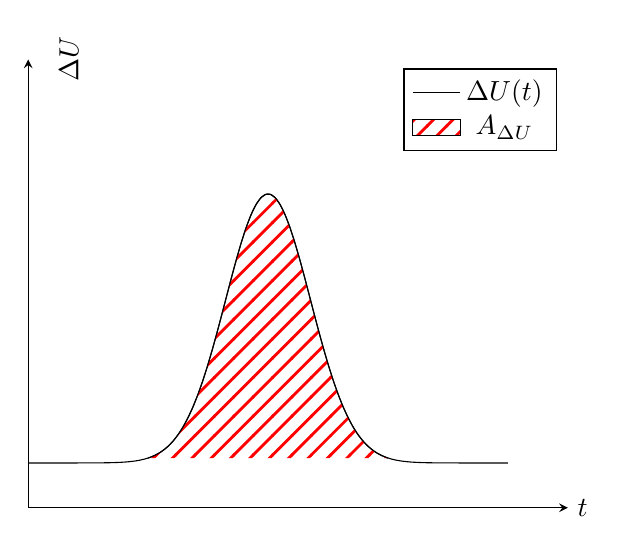
\begin{tikzpicture}
		\begin{axis}[domain=-1:7,
		samples=100,
		ymin=0, ymax=5	,	
		xmin=-1, xmax=8,	 
		axis lines=left,
		xtick=\empty,
		ytick=\empty,
		xlabel=$t$, xlabel style={at=(current axis.right of origin), anchor=west},
		ylabel=$\Delta U$, ylabel style={at=(current axis.above origin), anchor=south}]
		
		\addplot+[color=black,
		mark=none] {3*exp(-(x-3)^2) + 0.5};
		\addlegendentry{$\Delta U(t)$}
		\addplot+[mark=none,
		domain=1:5,
		samples=100,
		pattern=flexible hatch,
		hatch distance=8pt,
		hatch thickness=1pt,
		draw=black,
		pattern color=red,
		area legend]
		{3*exp(-(x-3)^2) + 0.5};
		\addlegendentry{$A_{\Delta U}$}
		\end{axis}
		\end{tikzpicture}
		\caption{}
		\label{fig:dsc-calibration_dU(t)}
	\end{subfigure}
	\hfill
	\begin{subfigure}{0.45\textwidth}
		\begin{tikzpicture}
		\begin{axis}[domain=-1:6.3,
		samples=100,
		ymin=0, ymax=5	,	
		xmin=-1, xmax=8,	 
		axis lines=left,
		xtick={2, 4},
		xticklabels={$T_{Kal,i}$, $T_{Kal,i+1}$},
		ytick=\empty,
		xlabel=$T$, xlabel style={at=(current axis.right of origin), anchor=west},
		ylabel=$sens$, ylabel style={at=(current axis.above origin), anchor=south}
		]
		
		\addplot+[color=black, mark=none] {3 - 0.1*x - 0.005*x^2};
		\addplot[only marks, mark=x, color=black] 
		table {0 3.
			1 2.9
			2 2.78
			4 2.53
			5 2.38
		};
		\end{axis}
		\end{tikzpicture}
		\caption{}
		\label{fig:dsc-calibration_sens(T)}
	\end{subfigure}
	\caption{Sensitivity calibration illustration graphs: (a) Computation of the area $A_{\Delta U}$ under the measuring signal $\Delta U(t)$ graph for a material with known melting point $T_{\text{Kal}}$ and enthalpy $\Delta H_{\text{Kal}}$. $A_{\Delta U}$ is related to melting enthalpy via factor $sens$. This is performed for several materials (In, Sn, Zn, Al) such that in (b) one can interpolate $sens=\frac{A_{\Delta U}}{\Delta H_{\text{Kal}}}$ for a certain temperature range. \\
	Cf. measurement data \cref{fig:measurement_csv_data}.}
\end{figure}

With the mapping $\varPhi(T_{ref}) = \frac{\Delta U(T_{ref})}{sens(T_{ref})}$ the heat flux into the sample then can be computed for a measurement signal $\Delta U$ of unknown materials. 

\paragraph{Measurement data}\mbox{}\\
In this context the measurements were performed as remarked at the AIT in Wien using the heat flux DSC \textit{Netzsch DSC 204 F1 Phoenix\textsuperscript{\textregistered}}. An excerpt of the .csv file which contains the measurement data for heat rate ${\beta=1.25 \frac{K}{min}}$ is shown in \cref{fig:measurement_csv_data}. Beside general information like date and time when the experiment was performed and which sample and crucibles have been used there are four columns. The first three of those contain the information recorded during the experiment, namely the temperature at the reference crucible $T_{ref}$, elapsed time $t$ since start of measurement set and electric potential $\Delta U_m$ caused by the temperature difference between reference and sample crucible. 
From the sensitivity calibration, the fourth column holds the sensitivity values $sens$.
Note here that $\Delta U_m$ is normalized on the sample mass such that is has unit $[\Delta U_m]=\frac{\mu V}{mg}$. We need to consider this for the following computation of the heat flux into the PCM

\begin{equation}
	\varPhi_q^{\eta_i}(T_{ref}^{\eta_i}) = m_{pcm} \cdot \frac{\Delta U_m(T_{ref}^{\eta_i})}{sens(T_{ref}^{\eta_i})}
\end{equation}

where $m_{pcm}$ is the sample mass, $\Delta U_m(T_{ref}^{\eta_i})$ is the voltage and $sens(T_{ref}^{\eta_i})$ the sensitivity at reference temperature $T_{ref}^{\eta_i}$ for measurement number $i$. \\
These measurement data are used later in the parameter estimation optimization problem in \cref{sec:optimization_problem}.


\begin{figure}[H]
	\centering
	\includegraphics[width=.8\textwidth]{/home/argo/masterarbeit/thesis/images/messdaten.png}
	\caption{Exemplary excerpt of measurement data .csv file for heat rate $\beta=1.25 \frac{K}{min}$. In the upper part measurement properties like measuring device or sample mass are listed. Below there are four columns with the measurement values: Temperature at reference crucible $T_{ref}$, elapsed time $t$ since start of measurement set, electric potential $\Delta U_m$ because of temperature difference between reference and sample crucible (normalized on sample mass) and sensitivity values $sens$ from sensitivity calibration. \\
	Cf. \cref{sec:heat_flux_dsc} paragraph sensitivity calibration.}
	\label{fig:measurement_csv_data}
\end{figure}


\subsubsection{Power compensated DSC}
\label{sec:power_compensated_dsc}
Another kind of differential scanning calorimetry is the
power compensated DSC (\cref{fig:DSC_power_compensated_principle}). 
The main difference to a heat flux DSC is that there are 2 separated chambers for a reference and the sample. Both have individual heaters and temperature sensors such that a feedback control system keeps the temperature in both chambers on the same value. Since the electrical power for heating is known the heat flux is gained due to energy conservation. \\


\subsection{Smearing Problem}
\label{sec:smearing_problem}
A common way to perform the heat flux DSC calibration, measurement and specific heat capacity $c_p$ computation is described in detail in DIN 11357 \cite{DIN_11357}. By assuming a proportionality between the heat flux into the sample and the sample's heat capacity one gets the equation

\begin{equation}
	c_p^S(T) = c_p^{R}(T) \cdot \frac{m^R}{m^S} \cdot \frac{\varPhi^S(T) - \varPhi^0(T)}{\varPhi^R(T) - \varPhi^0(T)}
	\label{eq:c_p_formula_DIN}
\end{equation}

where the indices $S$ and $R$ denote the sample respectively reference. Reference means here a material with known specific heat capacity $c_p^R(T)$, not to be mistaken with the reference side of the experimental setup which is usually empty. In our case this reference material is sapphire. Furthermore $m$ is the mass and $\varPhi^0$ is the heat flux if both crucibles are empty. $\varPhi^0$ is subtracted to compensate asymmetries in the experimental setup. \\
In \cref{fig:heat_flux_measurements} the measurement data of the heat flux into the PCM $\varPhi_q^{\eta}(T_{ref})$ is shown for all heat rates dependent on the temperature at the reference crucible. Using \cref{eq:c_p_formula_DIN} the computed specific heat capacities for the PCM are shown in \cref{fig:c_p_DIN_formula}. For higher heat rates the peak position shifts to higher temperatures and furthermore the peak is smeared out. This is known as the smearing problem since $c_p(T)$ is a material property and therefore independent of the heat rate.


\begin{figure}[H]
	\centering
	\begin{subfigure}{0.7\textwidth}
		\includegraphics[width=1.\textwidth]{/home/argo/masterarbeit/thesis/images/heat_flux_measurement.png}
		\caption{}
		\label{fig:heat_flux_measurements}
	\end{subfigure}
	\begin{subfigure}{0.7\textwidth}
		\includegraphics[width=1.\textwidth]{/home/argo/masterarbeit/thesis/images/c_p_DIN_formula.png}
		\caption{}
		\label{fig:c_p_DIN_formula}
	\end{subfigure}
	\caption{(a) Heat flux measurement values $\varPhi_q^{\eta}(T_{ref})$ and (b) computed specific heat capacity $c_p(T)$ using \cref{eq:c_p_formula_DIN} with distinct smearing effect for higher heat rates. \\
	Cf. Simulated heat flux (\cref{fig:smearing_effect_simulation_heat_flux}) and $c_p(T)$ obtained by parameter estimation depicted in \cref{fig:5Gaussians_all_c_p,fig:FS_all_c_p,fig:FS_all_c_p_modHeatRate}.}
\end{figure}


\newpage
\section{Mathematical background}
\label{sec:mathematical_background}

In this section the mathematical problems we treat in this thesis will be introduced, that is essentially the solution of (partial) differential equations and the nonlinear least squares problem. Further, methods for the numerical solution of these problems are shown. \\

Since crucial and occurring several times in this section, we introduce the initial value problem (IVP)

\begin{align}
	\dot{y} = f(y(t), t; p) \label{eq:initial_value_problem_definition} \\
	y(t_0) = y_0 \nonumber
\end{align}

with differential state vector $y \in \mathbb{R}^n$, time $t \in \mathbb{R}$ and parameters $p \in \mathbb{R}^{n_p}$. Function $f: \mathbb{R}^n \times \mathbb{R} \rightarrow \mathbb{R}^n$ assumed sufficiently smooth is called the differential equation's right hand side within the ordinary differential equation (ODE) $\dot{y} = f(y(t), t; p)$. The semicolon separates function arguments and  parameters\footnote{E.g., also controls $u$ in the context of optimal control.}. Initial time and state are $t_0$ and $y_0$, respectively. \\
Local existence of the solution is shown in theorem of Peano, basically requires continuity of $f$ (see e.g. \cite{ODE_analytic} Theorem 2.2.8).
For global existence and uniqueness the theorem of Picard-Lindelöf holds, requiring essentially $f$ Lipschitz continuous (see e.g. \cite{ODE_analytic} Theorem 2.4.5). \\





\subsection{Derivative generation}
In the context of continuous optimization we take advantage of derivative information in order to minimize some function. 
There are several possibilities to obtain these derivatives. We will introduce here the concept of finite differences and automatic differentiation which were used in this thesis. 
Beside them the methods of symbolic- and complex step-differentiation exist and are explained e.g. in \cite{diss_jan}.

\subsubsection{Finite differences}
\label{sec:finite_differences}
Derivatives approximated by finite differences are deployed beside the optimization task also in the spatial discretization of a partial differential equation which will be explained in more detail in \cref{sec:pde_discretization}.
They can be derived easily from Taylor-series expansion where we restrict ourselves to the scalar function argument case $x \in \mathbb{R}$ since derivatives in higher dimensions $x \in \mathbb{R}^n$ are obtained straight forward by applying directional derivatives under the assumption of total differentiability.  \\
Considering the function $f: \mathbb{R} \rightarrow \mathbb{R}$ with $f \in \mathcal{C}^2$ the Taylor series looks as follows:


\begin{equation}
f(x+h) = f(x) + h \cdot \frac{\partial f}{\partial x}(x) + \mathcal{O}(h^2)
\end{equation}

Reordering gives the one-sided derivative approximation

\begin{equation}
\frac{\partial f}{\partial x}(x) = \frac{f(x+h) - f(x)}{h} + \mathcal{O}(h)
\label{eq:one_sided_discretized_derivative}
\end{equation}

Regarding the Taylor series up to order two in both directions of the domain of definition,
\begin{subequations}
	\label{eq:finite_differences_taylor_exp}
	\begin{align}
	f(x+h) = f(x) + h \cdot \frac{\partial f}{\partial x}(x) + \frac{h^2}{2} \cdot \frac{\partial^2 f}{\partial^2 x}(x) + \mathcal{O}(h^3) \label{eq:finite_differences_taylor_exp_+} \\
	f(x-h) = f(x) - h \cdot \frac{\partial f}{\partial x}(x) + \frac{h^2}{2} \cdot \frac{\partial^2 f}{\partial^2 x}(x) + \mathcal{O}(h^3)  \label{eq:finite_differences_taylor_exp_-}	
	\end{align}
\end{subequations}


subtract both equations and reorder again we get

\begin{equation}
\frac{\partial f}{\partial x}(x) = \frac{f(x+h) - f(x-h)}{2 h} + \mathcal{O}(h^2)
\end{equation}

which has a higher error order, though at the expense of an additional function evaluation for the usual case where the function value $f(x)$ is evaluated . \\

Second order derivatives can be approximated analogously by adding \cref{eq:finite_differences_taylor_exp_+} and \cref{eq:finite_differences_taylor_exp_-}:

\begin{equation}
\frac{\partial^2 f}{\partial x^2}(x) = \frac{f(x-h) - 2 \cdot f(x) + f(x+h)}{h^2} + \mathcal{O}(h)
\label{eq:finite_difference_2nd_der}
\end{equation}

In the spatial discretization of partial differential equations one often choose a finer grid for areas of interest. So for the resulting non-equidistant grid (see \cref{fig:2_point_formula_illustration}) one needs a more general formula which is derived by considering again the Taylor expansion

\begin{subequations}
	\label{eq:finite_differences_taylor_exp_non-homogenous}
	\begin{align}
	f(x-h) = & f(x) - h \cdot \frac{\partial f}{\partial x}(x) + \frac{h^2}{2} \cdot \frac{\partial^2 f}{\partial x^2}(x) + \mathcal{O}(h^3) \label{eq:finite_differences_taylor_exp_non-homogenous_1} \\
	f(x+\alpha h) = & f(x) + \alpha h \cdot \frac{\partial f}{\partial x}(x) + \frac{\alpha^2 h^2}{2} \cdot \frac{\partial^2 f}{\partial x^2}(x) + \mathcal{O}(h^3)  \label{eq:finite_differences_taylor_exp_non-homogenous_2}
	\end{align}
\end{subequations}



Multiplying \cref{eq:finite_differences_taylor_exp_non-homogenous_1} with $\alpha$ and adding \cref{eq:finite_differences_taylor_exp_non-homogenous_2} gives

\begin{align}
\alpha f(x-h) + f(x+\alpha h) = \alpha f(x) + \alpha \frac{h^2}{2} \frac{\partial^2 f}{\partial x^2}(x) + f(x) + \frac{\alpha^2 h^2}{2} \frac{\partial^2 f}{\partial x^2}(x) + \mathcal{O}(h^3)  \\
\Leftrightarrow (\alpha+1) \frac{\alpha h^2}{2} \frac{\partial^2 f}{\partial x^2}(x) = \alpha f(x-h) - (\alpha+1) f(x) + f(x+\alpha h) + \mathcal{O}(h^3) 
\end{align}

\begin{equation}
\Leftrightarrow \frac{\partial^2 f}{\partial x^2}(x) = \frac{1}{h^2} \left[ \frac{2}{1+\alpha} f(x-h) - \frac{2}{\alpha} f(x) + \frac{2}{\alpha (\alpha+1)} f(x+\alpha h) \right] + \mathcal{O}(h) 
\label{eq:2_point_formula_inhomogeneous}
\end{equation} \\

Note that for a homogeneous grid ($\alpha=1$) this is obviously equal to \cref{eq:finite_difference_2nd_der}. \\

\begin{figure}[H]
	\centering
	\includegraphics[width=1.\textwidth]{/home/argo/masterarbeit/thesis/images/2nd_derivative_2-point_formula_illustration.png}
	\caption{Function $f(x)$ and its discretization $f_i$ on a non-equidistant grid.}
	\label{fig:2_point_formula_illustration}
\end{figure}


As mentioned before, for simplicity we restricted ourselves to functions of scalar argument $x \in \mathbb{R}$. In the case $x \in \mathbb{R}^n$ the Jacobian can be approximated by directional derivatives. So, e.g. for the one-sided first derivative \cref{eq:one_sided_discretized_derivative} $n+1$ function evaluations are necessary. In the case of a vector-valued function each component is considered separately. \\

The great advantage of finite differences is their simple implementation. We treat the function as a black box, perturb the input arguments a bit, perform $n+1$ function evaluations and get an approximation of the first derivative. \\
This simplicity is at the expense of accuracy. If we choose $h$ too small, cancellation occurs. Otherwise with $h$ large the remainder term of the Taylor expansion gets large. Therefore this error can be minimized by varying $h$, although then the derivative approximation is still not exact.




\subsubsection{Automatic Differentiation and Internal Numerical Differentiation}
\label{sec:Automatic_diff_IND_theory}
The basic idea of Automatic Differentiation (AD) is to subdivide a sufficiently smooth function ${f: \mathbb{R}^n \rightarrow \mathbb{R}^m}$ into so called elementary functions $\varphi_i$ of which the derivative is known. 

The evaluation of these elementary functions give intermediate values $v_i = \varphi_i(v_j)_{j \prec i}$ where the dependency relation $\prec$ is defined as

\begin{equation}
j \prec i \Leftrightarrow v_j \text{\textit{ is an argument of }} \varphi_i.
\end{equation}

By successively applying the chain rule one obtains the derivative of $f$.
One can distinguish the forward and reverse mode which will be explained in more detail now and exemplified by means of the example function

\begin{equation}
F(x) = 
\begin{bmatrix}
\exp((1+x_1)^2) + x_3 \\
x_2 \cdot \sin(1+x_1)
\end{bmatrix}
\label{eq:AD_example}
\end{equation}

For a profound view on the subject of automatic differentiation, see e.g. \cite{eval_derivatives_walther_griewank}.


\paragraph{Forward Mode}\mbox{}\\
In the forward mode, the directional derivative $\dot{y}$ is computed for a given direction $\dot{x}$ (i.e. $|| \dot{x} || = 1$) at an evaluation point $x$:

\begin{equation}
\dot{y} = \frac{\partial f}{\partial x}(x) \cdot \dot{x}
\end{equation}

Here the notation $\dot{x}$ is not to be mistaken with the time derivative often used in physics context.
The algorithm called \textit{first order forward sweep} (see \cref{tab:first_order_forward_sweep}) is structured into three parts. First the auxiliary variables $v_{1-n},...,v_0$ and $\dot{v}_{1-n},...,\dot{v}_0$ are initialized with the evaluation point $x$ and the direction of the directional derivative $\dot{x}$. So if we want to get $\frac{\partial f}{\partial x_2}$ we would need to set $\dot{x} = \begin{bmatrix}
0 & 1 & 0 & \dots & 0
\end{bmatrix}^T$. One can see here that with one forward sweep we get one column of the Jacobian $ \frac{\partial f}{\partial x}$. 
After the initialization the actual forward sweep begins where the $k$ elemental functions of $f$ are evaluated and saved in the intermediate values $v_i$. Simultaneously, their derivatives  $\dot{v}_i$ are computed using previously calculated intermediate values and derivatives. E.g., for $v_2 = \varphi_2(v_0, v_1)$ it holds $\dot{v}_2 = \frac{\partial \varphi_2}{\partial v_0} \dot{v_0} + \frac{\partial \varphi_2}{\partial v_1} \dot{v_1}$. \\
The last $m$ intermediate variables represent the solution vector. Finally this values and derivatives are extracted.



\begin{table}[H]
	\begin{tabular}{|c | l c l | l |} \hline
		Initialization & $[v_{i-n}, \dot{v}_{i-n}]$ & $=$ & $[x_i, \dot{x}_i]$ & $i=1,...,n$ \\ \hline
		Intermediate steps & $[v_{i}, \dot{v}_{i}]$ & $=$ & $[\varphi_i(v_j)_{j \prec i}, \sum_{j \prec i} \frac{\partial \varphi_i}{\partial v_j}(v_j) \cdot \dot{v}_j]$ & $i=1,...,k$ \\ \hline
		Extract solution & $[y_{m-i}, \dot{y}_{m-i}]$ & $=$ & $[v_{k-i}, \dot{v}_{k-i}]$ & $i=m-1,...,0$ \\ \hline
	\end{tabular}
	\caption{Algorithm of first order forward sweep. Elucidated in text above and exemplified in \cref{tab:AD_example_forward}.}
	\label{tab:first_order_forward_sweep}
\end{table}

In order to illustrate this algorithm is applied on the example function \cref{eq:AD_example}, see \cref{tab:AD_example_forward}:

\begin{table}[H]
	\centering
	\begin{tabular}{| c | l | l |} \hline
		Initialization & $v_{-2} = x_1$ & $\dot{v}_{-2} = \dot{x}_1$ \\
		& $v_{-1} = x_2$ & $\dot{v}_{-1} = \dot{x}_2$ \\
		& $v_{0} = x_3$ & $\dot{v_{0}} = \dot{x}_3$ \\ \hline
		Intermediate Steps & $v_1 = 1+v_{-2}$ & $\dot{v_1} = 1 \cdot \dot{v}_{-2}$ \\
		& $v_2 = v_{1}^2$ & $\dot{v_2} = 2 v_1 \cdot \dot{v}_{1}$ \\
		& $v_3 = \exp(v_{2})$ & $\dot{v_3} = \exp(v_2) \cdot \dot{v}_{2}$ \\
		& $v_4 = \sin(v_{1})$ & $\dot{v_4} = \cos(v_1) \cdot \dot{v}_{1}$ \\
		& $v_{5} = v_3 + v_0$ & $\dot{v_{5}} = 1 \cdot \dot{v}_3 + 1 \cdot \dot{v}_0$ \\
		& $v_{6} = v_{-1} \cdot v_4$ & $\dot{v_{6}} = \dot{v}_{-1} \cdot v_4 + v_{-1} \cdot \dot{v}_4$ \\ \hline
		Extract  solution & $y_1 = v_5$ & $\dot{y}_1 = \dot{v}_5$ \\
		& $y_2 = v_6$ & $\dot{y}_2 = \dot{v}_6$ \\ \hline
	\end{tabular}
	\caption{First order forward sweep (\cref{tab:first_order_forward_sweep}) applied on \cref{eq:AD_example}.}
	\label{tab:AD_example_forward}
\end{table}




\paragraph{Adjoint Mode}\mbox{}\\
Beside the forward mode there is the adjoint mode where the adjoint directional derivative $\bar{x}^T$ is computed for a given adjoint direction $\bar{y}^T$ at the evaluation point $x$. 

\begin{equation}
\bar{x}^T = \bar{y}^T \frac{\partial f}{\partial x}(x)
\end{equation}

The algorithm is shown in \cref{tab:first_order_adjoint_sweep} where operator $+ \hspace{-0.12cm} =$ is defined as $x + \hspace{-0.12cm} = y \ \Leftrightarrow \ x = x + y$. In contrary to the forward mode we need here an additional set of adjoint intermediate variables $\bar{v}_i$. These contain the adjoint sensitivity information which are initialized to zero in the first step. \\
The following forward sweep is analog to the one shown in \cref{tab:first_order_forward_sweep}, however here we compute just the intermediate function evaluations without derivatives. We need these function values in the next part. \\
The actual adjoint directional derivatives are now computed in the reverse sweep which consists of three sub-steps. First of all, the adjoint directions $\bar{y}$ are chosen. So for example, if we want the second row of the Jacobian $\frac{\partial f_2}{\partial x}$ we need to set $\bar{y} = \begin{bmatrix}
0 & 1 & 0 & \dots & 0
\end{bmatrix}^T$.
Next, all contributions to the adjoint intermediate variables will be successively summed up by applying the adjoint equation $\bar{y}^T \dot{y} = \bar{y}^T \frac{\partial f}{\partial x}(x) \cdot \dot{x} = \bar{x}^T \dot{x}$ in a reverse scheme (that is why we need the forward sweep and hence the intermediate value evaluations first). Finally, we can extract the solution $\bar{x}$ which corresponds to a row in $\frac{\partial f}{\partial x}$.


\begin{table}[H]
	\centering
	\begin{tabular}{| c | l c l | l |} \hline
		Initialization & $\bar{v}_i$ & $=$ & $0$ & $i=1-n,...,k-m$ \\ \hline
		& $v_{i-n}$ & $=$ & $x_i$ & $i=1,...,n$ \\
		Forward Sweep & $v_{i}$ & $=$ & $\varphi_i(v_j)_{j \prec i}$ & $i=1,...,k$ \\
		& $y_{m-i}$ & $=$ & $v_{k-i}$ & $i=m-1,...,0$ \\ \hline
		& $\bar{v}_{k-i}$ & $=$ & $\bar{y}_{m-i}$ & $i=0,...,m-1$ \\
		Reverse Sweep & $\bar{v}_j$ & $+ \hspace{-0.1cm} =$ & $\bar{v}_i \frac{\partial \varphi_i}{\partial v_j}(v_j) \quad \forall \ j \prec i$ & $i=k,...,1$ \\
		& $\bar{x}_i$ & $=$ & $\bar{v}_{i-n}$ & $i=n,...,1$ \\ \hline
	\end{tabular}
	\caption{Algorithm of first order adjoint sweep. Elucidated in text above and exemplified in \cref{tab:AD_example_adjoint}.}
	\label{tab:first_order_adjoint_sweep}
\end{table}

Again we apply this algorithm on the exemplary function \cref{eq:AD_example}:

\begin{table}[H]
	\centering
	\begin{tabular}{| c | l | l |} \hline
		& \textbf{Forward Sweep} & \textbf{Reverse Sweep} \\ \hline
		Initialization & $v_{-2}=x_1$ & $\bar{v}_6=\bar{y}_2$ \\
		& $v_{-1}=x_2$ & $\bar{v}_5=\bar{y}_1$ \\
		& $v_{0}=x_3$ & $\bar{v}_4=...=\bar{v}_{-2}=0$ \\	\hline
		Sweep & $v_1=1+v_{-2}$ & $\bar{v}_{-1} +\hspace{-0.1cm}= \bar{v}_6 \cdot v_4$ \\
		& $v_2=v_{1}^2$ & $\bar{v}_{4} \ \ +\hspace{-0.1cm}= \bar{v}_6 \cdot v_{-1} $ \\
		& $v_3=\exp(v_2)$ & $\bar{v}_{3} \ \ +\hspace{-0.1cm}= \bar{v}_5 \cdot 1 $ \\
		& $v_4= \sin(v_1)$ & $\bar{v}_{0} \ \ +\hspace{-0.1cm}= \bar{v}_5 \cdot 1 $ \\
		& $v_5=v_{3} + v_0$ & $\bar{v}_{1} \ \ +\hspace{-0.1cm}= \bar{v}_4 \cdot \cos(v_1) $ \\
		& $v_6=v_{-1} \cdot v_4$ & $\bar{v}_{2} \ \ +\hspace{-0.1cm}= \bar{v}_3 \cdot \exp(v_2) $ \\
		& & $\bar{v}_1 \ \ +\hspace{-0.1cm}= \bar{v}_2 \cdot 2 v_1$ \\
		& & $\bar{v}_{-2} +\hspace{-0.1cm}= \bar{v}_1 \cdot 1$	\\ \hline
		Extract solution & $y_1 = v_5$ & $\bar{x}_3 = \bar{v}_0$ \\
		& $y_2 = v_6$ & $\bar{x}_2 = \bar{v}_{-1}$ \\
		& & $\bar{x}_1 = \bar{v}_{-2}$	\\ \hline
	\end{tabular}
	\caption{First order adjoint sweep (\cref{tab:first_order_adjoint_sweep}) applied on \cref{eq:AD_example}}
	\label{tab:AD_example_adjoint}
\end{table} 


Until now, the fundamental principles of AD have been explained, in particular just the first order derivative in forward and adjoint mode. Higher derivatives of arbitrary order can be obtained for example by the method of Taylor Coefficient Propagation (fundamentals in \cite{TC-prop_basis} and applied in \cite{diss_jan}). \\

In this thesis we are actually interested in the sensitivities of the solution of an IVP \cref{eq:initial_value_problem_definition} with respect to parameters $p$, namely $\frac{\partial y}{\partial p}$. 
This can be done by solving the variational differential equation (see e.g. \cite{diff_equations_numerics}) which can be derived as follows using the integral form of the IVP and assuming $f$ continuously differentiable. Initial values $y_0$ are assumed to be independent of $p$ here.

\begin{align}
	y(t;p) = \ & y_0 + \int_{t_0}^{t} f(y(\tau;p),\tau;p) \ d\tau \\
	\Rightarrow \frac{\partial y}{\partial p} = & \int_{t_0}^{t} \left[ \frac{\partial f}{\partial y} \cdot \frac{\partial y}{\partial p} + \frac{\partial f}{\partial p} \right] d\tau \nonumber
\end{align}

Function arguments of the partial derivatives are omitted here for better readability. Taking the derivative with respect to time on both sides gives the corresponding initial value problem

\begin{align}
	\frac{\partial}{\partial t} \left( \frac{\partial y}{\partial p} \right) = \ & \frac{\partial f}{\partial y} \cdot \frac{\partial y}{\partial p} + \frac{\partial f}{\partial p} \\
	\frac{\partial y}{\partial p}(t_0) = \ & 0 \nonumber
\end{align}

Solving this IVP together with the nominal trajectory is one possibility to get $\frac{\partial y}{\partial p}$. If $y \in \mathbb{R}^n$ and $p \in \mathbb{R}^{n_p}$ the total differential equation system to solve would consist of $n + n \cdot n_p$ equations which is a computationally costly approach. \\
Another method uses Internal Numerical Differentiation (IND). Since the numerical integrator uses a stepsize control in order to limit the relative local error, the idea of IND is to freeze these adaptive components such that the integrator is differentiable. 
Applying AD then means treating all mathematical operations of the used integration scheme as elemental operations. So it is basically straight forward to apply the chain rule on all these elemental operations in order to get the derivative $\frac{\partial y}{\partial p}$ just as explained above. 
The application of AD is advantageous because one obtains exact numerical derivatives while the computed differential equation's nominal trajectory is still error controlled. \\
The details on IND including the generation of higher derivatives via taylor coefficient propagation are elucidated in \cite{diss_jan} which is also the basis of the software package SolvIND used in \cref{sec:numerical_experiments} for the numerical experiments.


\subsection{Numerical solution of initial value problems}
\label{sec:theory_ODE_solver_BDF}

In this section numerical methods will be introduced to solve initial value problems of the form given in \cref{eq:initial_value_problem_definition} without parameters $p$. \\ 
There are a lot of different methods for the numerical solution of an IVP (see e.g. \cite{diff_equations_numerics}) like Runge-Kutta (RK) or linear multistep methods (LMM). The solver we used in this thesis applies the method of Backward Differentiation Formulas (BDF) which will be explained further now, assuming the differential equation's right hand side $f \in \mathcal{C}^1$. \\
Basic idea of the BDF method of order $k$ is to interpolate the last $(k+1)$ solution points $y_m,...,y_{m+k}$ with a polynomial such that the unknown point $y_{m+k}$ satisfies the ODE at $t_{m+k}$. 
It is defined as

\begin{equation}
	\sum_{i=0}^{k} \alpha_{im} y_{m+i} = h_{m+k-1} f(y_{m+k},t_{m+k})
	\label{eq:bdf_formula}
\end{equation}

where $\alpha_{ij} \in \mathbb{R}$ with $\alpha_{0m},\alpha_{km} \ne 0 \ \forall \ m$ are the method's coefficients. BDF methods up to order 6 are used in practice because these are zero-stable. \\
Since \cref{eq:bdf_formula} is a nonlinear system of equations it is solved iteratively using Newton's method (therefore we need $f \in \mathcal{C}^1$). In order to obtain a good starting point a so called predictor is used, which is the integration polynomial of the previous integration step. With this initial guess for $y_{m+k}$ the Newton method can be applied to get the so called corrector polynomial, which satisfies the differential equation at $t_{m+k}$. \\
As we want the numerical integrator both to perform large integration steps to minimize the required time to solve the IVP and limit the inevitable numerical errors to a predefined value we are dependent on a strategy to choose the step width $h_{m+k-1}$ accordingly. This is done by estimating the local error (see e.g. \cite{diss_jan} page 128) in each integration step. Either the local error is smaller than some tolerance then the step width might be increased in the next integration step, otherwise decreased until the local error tolerance is satisfied. \\

The BDF solver DAESOL-II embedded in SolvIND has been used in this thesis to solve \cref{eq:heat_equation_discretized}.


%The stated methods solve the initial value problem in an iterative manner, in contrary to collocation where the problem can be solved in one big system




\subsection{Partial differential equation discretization in space: Method of lines}
\label{sec:pde_discretization}


Given a partial differential equation (PDE) with the sought solution $u(x,t)$ dependent on space coordinate $x$ and time $t$. Since the problem of finding $u(x,t)$ that solves the corresponding PDE is infinite-dimensional, a method of discretizing space and time is introduced in the following in order to obtain a finite-dimensional problem. \\
Since later in \cref{sec:simulation_of_DSC} the heat conduction problem shall be solved, in this section we treat a boundary value problem (BVP) of the following analog form:

\begin{subequations}
	\begin{align}
	\frac{\partial u}{\partial t}(x,t) & - \alpha(u(x,t)) \cdot \frac{\partial^2 u}{\partial x^2}(x,t) = 0 & \forall x \in [a,b], \ t \in [t_0,t_f] \label{eq:method_of_lines_pde} \\
	u(a,t) & = u_a(t)  & \forall t \in [t_0,t_f] \label{eq:method_of_lines_dirichlet} \\
	\frac{\partial u}{\partial x}(b,t) & = 0  & \forall t \in [t_0,t_f] \label{eq:method_of_lines_neumann}  \\
	u(x,t_0) & = u_{init}(x) & \forall x \in [a,b] \label{eq:method_of_lines_start}
	\end{align}
	\label{eq:method_of_lines}
\end{subequations}

on the domain $x \in [a,b] = \Omega \subseteq \mathbb{R}$ and $t \in [t_0,t_f] \subseteq \mathbb{R}$. \Cref{eq:method_of_lines_pde} is the 1D parabolic partial differential equation with $\alpha(u(x,t)) > 0$ (cf. heat equation \eqref{eq:heat_eq_derivation_1}), \cref{eq:method_of_lines_dirichlet} is the Dirichlet boundary condition at $x=a$, \cref{eq:method_of_lines_neumann} respectively the Neumann boundary condition at $x=b$ and lastly \cref{eq:method_of_lines_start} are the initial values at ${t=t_0}$. \\
Remark: This BVP is a special case and crucial for us in this thesis. For a more general view on the numerical solution of PDEs especially method of lines see e.g. \cite{pde_buch_solin}. \\

In order to make this boundary value problem numerically solvable the idea of method of lines is to keep the temporal variable $t$ continuous while space coordinate $x$ is discretized. Thus the PDE is transformed into an ODE. Here we use the spatial grid
\begin{align}
	x_k = a + k \cdot h & & k=0,...,N
\end{align}

with $x_{N} = b$ and for simplicity equidistant gridsize $h = \frac{b - a}{N}$. Evaluated on this grid the sought functions are
\begin{align}
	u_k(t) := u(x_k,t) & & k=0,...,N
\end{align}

only dependent on time $t$. Spatial derivatives in the PDE \eqref{eq:method_of_lines_pde} are then discretized using finite differences, see \cref{sec:finite_differences}. Here we apply
\begin{align}
	\frac{\partial^2 u}{\partial x^2}(x_k,t) \approx \frac{u_{k-1}(t) - 2 u_k(t) + u_{k+1}(t)}{h^2} & & k=1,...,N-1
	\label{eq:discretized_second_derivative}
\end{align}

Dirichlet boundary condition \cref{eq:method_of_lines_dirichlet} is applied by
\begin{align}
	u_0(t) & = u_a(t) \\
	\Rightarrow \ \dot{u}_0(t) & = \dot{u}_a(t)
\end{align}

and Neumann boundary condition \cref{eq:method_of_lines_neumann} by
\begin{align}
	\frac{\partial u}{\partial x}(b,t) & \approx \frac{u_{N} - u_{N-1}}{h} = 0 \nonumber \\
	\Leftrightarrow & \ u_{N-1} = u_{N} \label{eq:method_of_lines_neumann_applied}
\end{align}

The initial values in \cref{eq:method_of_lines_start} are discretized given as
\begin{align}
	u_k(t=t_0) = u_{init}(x_k) & & k = 0,...,N
\end{align}

Putting all these together, where due to the equality in \cref{eq:method_of_lines_neumann_applied} $u_{N}$ is omitted, we obtain the initial value problem 

\begin{align}
	\frac{d}{dt}
	\begin{pmatrix}
		u_0(t) \\
		u_1(t) \\
		\\
		\vdots \\
		\\
		u_{N-2}(t) \\
		u_{N-1}(t)
	\end{pmatrix}
	= & \
	\begin{pmatrix}
	0 \\
	\alpha(u_1(t)) \\
	\\
	\vdots
	\\
	\\
	\alpha(u_{N-2}(t)) \\
	\alpha(u_{N-1}(t))
	\end{pmatrix}
	.* \left[
	\begin{pmatrix}
		0 & & ... & & 0 \\
		1 & -2 & 1 \\
		\\
		& \ddots & \ddots & \ddots \\
		\\
		& & 1 & -2 & 1 \\
		& & & 1 & -1
	\end{pmatrix}
	\begin{pmatrix}
	u_0(t) \\
	u_1(t) \\
	\\
	\vdots \\
	\\
	u_{N-2}(t) \\
	u_{N-1}(t)
	\end{pmatrix} \right]
	+
	\begin{pmatrix}
		\dot{u}_a(t) \\
		0 \\
		\\
		\vdots \\
		\\
		\\
		0
	\end{pmatrix} \\
	u_k(t_0) = & \ u_{init}(x_k) \qquad \text{for} \ k = 0,...,N-1 \nonumber
\end{align}
 
where operator $.*$ is a row-wise multiplication, i.e. for vectors $v, w \in \mathbb{R}^n$ it holds $(v \ .* \ w)_i = v_i \cdot w_i$ for component $i$. This system can be solved by an appropriate ODE solver (see \cref{sec:theory_ODE_solver_BDF}) where the temporal discretization occurs. \\
Note that we discussed here for simplicity the case of an equidistant spatial grid. The numerical experiments were done with a heterogeneous grid (\cref{sec:spatial_discretization_grid}) which modifies the discretized second derivative equation \eqref{eq:discretized_second_derivative}, see \cref{eq:2_point_formula_inhomogeneous}. \\
The method of lines was applied in this thesis in \cref{sec:mathematical_model}.


%Given a partial differential equation (PDE) in the differential variable $u(t,x)$ (e.g. temperature dependent on time $t \in \mathbb{R}$ and space coordinate $x \in \Omega \subseteq \mathbb{R}^D$ with $D=\{1,2,3\}$). The method of lines is used to discretize the PDE in space such that with $N$ discretization points we get $N$ differential variables only dependent in time:
%
%\begin{equation}
%	u(x,t) \ \rightarrow \ \{ u_0(t), u_1(t), ..., u_{N-1}(t) \}
%\end{equation}
%
%This is illustrated in \cref{fig:pde_discretization_method_of_lines} in one space dimension $x$ at time $\hat{t}$.
%
%
%Spatial derivatives within the PDE are approximated using the finite difference formulas derived in \cref{subsubsec:finite_differences}. \\
%The differential variables $u_i$ of the resulting system are then just dependent on time $t$ such that we have an ODE system now. The PDE's boundary conditions (BC) are applied by using the differential variables at the border, in the 1D case this would be obviously $u_0$ and $u_{N-1}$. \\
%Dirichlet boundary conditions 
%\begin{equation}
%u(x_0, t) = u_0^{BC}(t)
%\end{equation}
%
%which fix the function value are applied by
%
%\begin{align}
%	u_0(t) & = u_0^{BC}(t) \\
%	\Leftrightarrow \dot{u}_0(t) & = \dot{u}_0^{BC}(t) \nonumber
%\end{align}
%
%On the other hand Neumann boundary conditions
%
%\begin{equation}
%	\nabla u(x_{0},t) = J_u
%\end{equation}
%
%setting the flux into the spatial domain $\Omega$ to a certain value
%
%\begin{align}
%	\frac{u_{1} - u_{0}}{x_{1} - x_{0}} = J_u  \\
%	\Leftrightarrow u_0 = u_1 + J_u (x_1 - x_0) \nonumber
%\end{align}
%
%The function value of $u_0$ is already defined by $u_1$ so $\dot{u}_0$ is not necessary.




\subsection{Optimization task: Parameter estimation}

In this section at first general results of optimization theory are introduced. Afterwards we will focus on nonlinear least squares problems which are used in the context of parameter estimation and solved numerically with the method of Gauss-Newton.

\subsubsection{General nonlinear program and optimality criteria}
\label{sec:optimization_theory_NLP}
In this section we first treat the general nonlinear optimization problem (NLP) of the form

\begin{align}
	\min_x & \ f(x) \label{eq:NLP_formulation} \\
	s.t. & \ F_2(x) = 0 \nonumber \\
	& \ F_3(x) \ge 0 \nonumber
\end{align}

where $x \in \mathbb{R}^n$ is the optimization variable, $f\text{: } \mathbb{R}^n \rightarrow \mathbb{R}$ is the objective function, $F_2\text{: } \mathbb{R}^n \rightarrow \mathbb{R}^{m_2}$ and $F_3\text{: } \mathbb{R}^n \rightarrow \mathbb{R}^{m_3}$ are the equality and inequality constraints, respectively. $f$, $F_2$ and $F_3$ are assumed sufficiently smooth. Index $m_1$ is missing because we will need this later in the context of a least squares problem. The results shown in this chapter can be found for example in \cite{nonlinear_optimiziation_wright}. \\

The Lagrange function of \cref{eq:NLP_formulation} is defined as

\begin{equation}
	\mathcal{L}(x,\lambda,\mu) := f(x) - \lambda^T F_2(x) - \mu^T F_3(x)
\end{equation}

with Lagrange multipliers $\lambda \in \mathbb{R}^{m_2}$ and $\mu \in \mathbb{R}^{m_3}$. \\

Before stating the major results from optimization theory we introduce the following definitions:

\begin{Definition}
	$S := \{ x \ | \ F_2(x) = 0 \ \text{and} \ F_3(x) \ge 0 \}$ is called \underline{feasible set}.
\end{Definition}

\begin{Definition}
	A feasible point $x^* \in S$ is called \underline{local minimum}, if there exists an $\epsilon > 0$ such that $f(x^*) \le f(x) \ \forall \ x \in S \cap \mathcal{B}(x^*, \epsilon)$. \\
	$\mathcal{B}(x^*, \epsilon)$ is a ball with center $x^*$ and radius $\epsilon$. \\
	If the inequality holds strictly, $x^*$ is called a \underline{strict local minimum}.
\end{Definition}

\begin{Definition}
	$I(x) := \{ i=1,...,m_3 \ | \ F_{3,i}(x) = 0 \}$ is called \underline{active set} with $s := \vert I \vert$.
\end{Definition}

\begin{Definition}
	$\tilde{F}_2(x) := 
	\begin{pmatrix}
		F_2(x) \\
		F_{3,i}(x), \ i \in I(x) 
	\end{pmatrix}$
	are the \underline{active constraints}.
\end{Definition}

\begin{Definition}
	$x$ is called \underline{regular} if linear independence constraint qualification [LICQ] is satisfied, i.e. $rank \left( \frac{\partial \tilde F_2(x)}{\partial x} \right) = m_2 + s$
\end{Definition}

\begin{Definition}
	\textbf{(Tangent space)} \\
	$T(x) := \left\{ p \in \mathbb{R}^n \ | \ \frac{\partial \tilde F_2(x)}{\partial x} \cdot p = 0 \right\}$ \\
	$T^+(x) := \left\{ p \in \mathbb{R}^n \ | \ \frac{\partial F_2(x)}{\partial x} \cdot p = 0, \frac{\partial F_{3,i}(x)}{\partial x} \cdot p = 0 \text{ for } i \in I(x) \ \text{with } \mu_i > 0 \right\}$ \\
	are called \underline{tangent space}. It holds $T(x) \subseteq T^+(x)$.
\end{Definition}

Major results from optimization theory are the necessary optimality conditions [NOC]

\begin{Theorem}
	$[\text{\textbf{NOC}}]$ \\
	Let $x^* \in S$ be a local minimum and regular, then it holds
	\begin{enumerate}
		\item \textbf{First order necessary optimality conditions [NOC1]} \\
		$\exists \lambda^* \in \mathbb{R}^{m_2}, \mu^* \in \mathbb{R}^{m_3}, \mu^* \ge 0$ s.t. \\
		$\nabla_x \mathcal{L}(x^*, \lambda^*, \mu^*) = 0$ and \\
		$(\mu^*)^T \cdot F_3(x^*) = 0$ (complementary condition [CC])
		\item \textbf{Second order necessary optimality condition [NOC2]} \\
		$p^T \nabla_x^2 \mathcal{L}(x^*, \lambda^*, \mu^*) p \ge 0 \ \forall \ p \in T(x^*)$
	\end{enumerate}
\end{Theorem}

and the sufficient optimality condition [SOC]

\begin{Theorem}
	$[\text{\textbf{SOC}}]$ \\
	Let $x^* \in S$ and let there exist $\lambda^*, \mu^* \ge 0$ such that $\nabla_x \mathcal{L}(x^*, \lambda^*, \mu^*) = 0$ and \\ $(\mu^*)^T \cdot F_3(x^*) = 0$. 
	Let $p^T \nabla_x^2 \mathcal{L}(x^*, \lambda^*, \mu^*) p > 0$ for $p \in T^+(x^*) \backslash \{0\}$. \\
	Then: $x^*$ is a strict local minimum.
\end{Theorem}

Finally we introduce for later usage 

\begin{Definition} \textbf{KKT-conditions} \\
	Feasibility and [NOC1] are called \underline{Karush-Kuhn-Tucker (KKT)-conditions}. \\
	A tuple $(x^*, \lambda^*, \mu^*)$ satisfying the KKT-conditions is called \underline{KKT-point}.
\end{Definition}


\subsubsection{Nonlinear least squares problem and Gauss-Newton method}
\label{sec:Gauss_Newton}
Since the thesis contains parameter estimation problems we will treat now the equality and inequality constrained nonlinear least squares problem

\begin{align}
	\min_x \ & \frac{1}{2}|| F_1(x) ||_2^2 \label{eq:least_squares_problem} \\
	s.t. \ & F_2(x) = 0 \nonumber \\
	& F_3(x) \ge 0 \nonumber
\end{align}

with $x \in \mathbb{R}^n$, residuum vector $F_1: \mathbb{R}^n \rightarrow \mathbb{R}^{m_1}$, equality constraints $F_2: \mathbb{R}^n \rightarrow \mathbb{R}^{m_2}$ and inequality constraints $F_3: \mathbb{R}^n \rightarrow \mathbb{R}^{m_3}$ and let $F_i \in \mathcal{C}^3$ for $i=\{1,2,3\}$.
Instead of applying the KKT-conditions on \cref{eq:least_squares_problem} we apply the method of Gauss-Newton (GN). \\
I.e., we solve this problem iteratively by updating an initial point $x^{(0)}$ with a sequence of solutions $\Delta x^{(k)}$ in iteration $k$ from linearized subproblems of the form

\begin{align}
\min_{\Delta x^{(k)}} \ & \frac{1}{2}|| F_1(x^{(k)}) + J_1(x^{(k)}) \Delta x^{(k)} ||_2^2 \label{eq:least_squares_problem_linearized} \\
s.t. \ & F_2(x^{(k)}) + J_2(x^{(k)}) \Delta x^{(k)} = 0 \nonumber \\
& F_3(x^{(k)}) + J_3(x^{(k)}) \Delta x^{(k)} \ge 0 \nonumber
\end{align}

with $J_1(x^{(k)}) := \frac{\partial F_1}{\partial x}(x^{(k)}) \in \mathbb{R}^{m_1 \times n}$, $J_2(x^{(k)}) := \frac{\partial F_2}{\partial x}(x^{(k)}) \in \mathbb{R}^{m_2 \times n}$ and $J_3(x^{(k)}) := \frac{\partial F_3}{\partial x}(x^{(k)}) \in \mathbb{R}^{m_3 \times n}$. Advantageous here is that we can avoid the computationally costly Hessian of the objective function. The iteration using the Gauss-Newton step $\Delta x^{(k)}$ in iteration $k$ then reads as

\begin{equation}
x^{(k+1)} = x^{(k)} + t^{(k)} \Delta x^{(k)}
\label{eq:Gauss_Newton_iteration}
\end{equation}

with stepsize $t^{(k)} \in (0,1]$ for global convergence, i.e. convergence to a local minimum from an arbitrary initial point $x^{(0)}$ (see \cref{sec:GN_numerical_solution}). Crucial is the equivalence of the solution $x^*$ of \cref{eq:least_squares_problem,eq:least_squares_problem_linearized} which is shown in \cite{diss_bock} Lemma 3.1.18.
In the following we will omit the function argument and iteration index for better readability, i.e. $F_i(x^{(k)}) \equiv F_i$ and $J_i(x^{(k)}) \equiv J_i$ for $i \in \{1,2,3\}$. \\

Applying KKT conditions on the linearized problem \cref{eq:least_squares_problem_linearized} gives the system

\begin{equation}
	\begin{bmatrix}
		J_1^T J_1 & -\tilde{J}_2^T \\
		\tilde{J}_2 & 0
	\end{bmatrix}
	\begin{bmatrix}
		\Delta x \\
		\tilde{\lambda}
	\end{bmatrix}
	= -
	\begin{bmatrix}
	J_1^T F_1 \\
	\tilde{F}_2
	\end{bmatrix}
	\label{eq:GN_KKT_system}
\end{equation}

with active constraints $\tilde{F_2}$ and corresponding Jacobian $\tilde{J}_2$ since inactive inequality constraints do not contribute to the computation of $\Delta x$ as their Lagrange multiplier is zero. The solution $\Delta x$ therefore reads as

\begin{align}
	\Delta x & =
	- \underbrace{\begin{pmatrix}
		\mathbbm{1} & 0
	\end{pmatrix}
	\begin{pmatrix}
		J_1^T J_1 & \tilde{J}_2^T \\
		\tilde{J}_2 & 0
	\end{pmatrix}^{-1}
	\begin{pmatrix}
		J_1^T & 0 \\
		0 & \mathbbm{1}
	\end{pmatrix}}_{=: J^+}
	\begin{pmatrix}
		F_1 \\
		\tilde{F}_2
	\end{pmatrix}
	\label{eq:GN_solution_formal}
\end{align}

with the generalized inverse $J^+ \equiv J^+(x^{(k)})$. An important result \cite{diss_bock} is

\begin{Lemma} \textcolor{white}{.}\\
	If $rank(\tilde{J}_2) = m_2+s$ and $rank 
	\begin{pmatrix}
	J_1 \\
	\tilde{J}_2
	\end{pmatrix}
	= n$,
	then 	
	$\begin{pmatrix}
		J_1^T J_1 & -\tilde{J}_2^T \\
		\tilde{J}_2 & 0
	\end{pmatrix}$
	is non-singular.
\end{Lemma}

\subsubsection{Numerical solution}
\label{sec:GN_numerical_solution}

For the numerical solution of the linear least squares subproblem \cref{eq:least_squares_problem_linearized} we will successively introduce the unconstrained, the equality constrained and finally the general equality and inequality constrained case because they are built up on each other, cf. \cite{numerical_methods_lsq_Bjorck}. Before that, we discuss methods for global convergence in order to be independent of a good initial point $x^{(0)}$. \\
In this context a \textit{level function} $T(x^{(k)})$ is introduced which must be decreased in each iteration. For the general equality and inequality constrained case, the choice

\begin{equation}
	T_1(x^{(k)}) = \frac{1}{2} || F_1(x^{(k)}) ||_2^2 + \sum_{i=1}^{m_2} \beta_i | F_{2,i}(x^{(k)}) | + \sum_{i=1}^{m_3} \gamma_i | \min\{0,F_{3,i}(x^{(k)})\} |
\end{equation}

with $\beta_i > |\lambda_i|$ and $\gamma_i > |\mu_i|$, i.e. larger than the absolute value of the corresponding Lagrange multiplier, guarantees global convergence to a local minimum under certain conditions, see \cite{diss_bock} theorem 3.2.6. \\
Finding an appropriate sequence of stepsizes $\{ t^{(k)} \}$ is in general known as \textit{line search} and there are a lot of different strategies to achieve this (see e.g. \cite{nonlinear_optimiziation_wright}). Examples are the Armijo strategy to ensure a sufficient decrease of the level function or the restrictive monotonicity test (RMT) \cite{bock2000_RMT} which is based on an estimate of the function curvature $\omega$. \\

The function argument and iteration index is omitted again in the following paragraphs except for the active set strategy for better legibility.

\paragraph{Unconstrained case}\mbox{}\\
In the unconstrained case we want to solve the problem

\begin{equation}
\min_{\Delta x} \frac{1}{2} || F_1 + J_1 \Delta x ||_2^2
\label{eq:numerical_solution_LSQ}
\end{equation}

Based on decomposing $J_1$ two solution strategies are shown (cf. \cite{nonlinear_optimiziation_wright} chapter 10.1) :

\begin{itemize}
	\item \textbf{QR decomposition} \\
	First $J_1$ is decomposed using a column pivoting QR factorization
	\begin{equation}
		J_1 P = Q R = 
		\begin{pmatrix}
			Q1 & Q2
		\end{pmatrix}
		\begin{pmatrix}
			\bar{R} \\
			0
		\end{pmatrix}
	\end{equation}
	where $Q \in \mathbb{R}^{m_1 \times m_1}$ is an orthogonal matrix split into $Q_1 \in \mathbb{R}^{m_1 \times n}$ and $Q_2 \in \mathbb{R}^{m_1 \times (m_1-n)}$. Further, $R \in \mathbb{R}^{m_1 \times n}$ with $\bar{R} \in \mathbb{R}^{n \times n}$ upper triangular matrix. Lastly $P \in \mathbb{R}^{n \times n}$ is a permutation matrix and therefore orthogonal. Inserting into the objective function \cref{eq:numerical_solution_LSQ} and omitting factor $\frac{1}{2}$ gives
	
	\begin{align}
		|| F_1 + J_1 \Delta x ||_2^2 & = || Q^T (F_1 + J_1 P P^T \Delta x) ||_2^2 = || Q^T F_1 + Q^T Q R P^T \Delta x ||_2^2 \\
		& = \left| \left| \begin{pmatrix}
		Q_1^T F_1 \\
		Q_2^T F_1
		\end{pmatrix} + 
		\begin{pmatrix}
		\bar{R} \\
		0
		\end{pmatrix}
		P^T \Delta x \right| \right|_2^2 \nonumber \\
		& = || Q_1^T F_1 + \bar{R} P^T \Delta x ||_2^2 + ||Q_2^T F_1 ||_2^2 \nonumber
	\end{align}
	
	If $rank(J_1)=n$ and therefore $\bar{R}$ has positive diagonal elements (\cite{numerical_methods_lsq_Bjorck} theorem 1.3.4) and is invertible  one can solve for $\Delta x$ since $\bar{R}$ is triangular:
	
	\begin{equation}
		\bar{R} P^T \Delta x = -Q_1^T F_1
	\end{equation}
	
	For the rank-deficient case see e.g. \cite{numerical_methods_lsq_Bjorck} chapter 1.3.2.
		
		
		
	\item \textbf{Singular value decomposition} \\
	Using a singular value decomposition (SVD) $J_1$ decomposes to
	\begin{equation}
		J_1 = U \Sigma V^T =
		\begin{pmatrix}
			U_1 & U_2
		\end{pmatrix}
		\begin{pmatrix}
			\bar{\Sigma} \\
			0
		\end{pmatrix}
			V^T
	\end{equation}
	
	with $U \in \mathbb{R}^{m_1 \times m_1}$ orthogonal split into $U_1 \in \mathbb{R}^{m_1 \times n}$ and $U_2 \in \mathbb{R}^{m_1 \times (m_1 - n)}$, $V \in \mathbb{R}^{n \times n}$ orthogonal and $\Sigma \in \mathbb{R}^{m_1 \times n}$ with $\bar{\Sigma} \in \mathbb{R}^{n \times n}$ diagonal. Let $r := rank(J_1)$. Then $\bar{\Sigma}$ has the singular values $\sigma_1 \ge \sigma_2 \ge ... \ge \sigma_r > 0$ and $\sigma_{r+1}=...=\sigma_{n} = 0$ on the diagonal. \\
	Inserting modifies the objective function of \cref{eq:numerical_solution_LSQ} where we omit again factor $\frac{1}{2}$ by
	
	\begin{align}
		|| F_1 + J_1 \Delta x ||_2^2 & = || F_1 + U \Sigma \overbrace{V^T \Delta x}^{=: \Delta y} ||_2^2 = || U ( U^T F_1 + \Sigma \Delta y ||_2^2 \label{eq:numerical_solution_LSQ_SVD} \\
		& = \left| \left| \begin{pmatrix}
		U_1^T F_1 \\
		U_2^T F_1
		\end{pmatrix} + 
		\begin{pmatrix}
		\bar{\Sigma} \\
		0
		\end{pmatrix}
		\Delta y \right| \right|_2^2 \nonumber \\
		& = || \underbrace{U_1^T F_1}_{=: c} + \bar{\Sigma} \Delta y ||_2^2 + || U_2^T F_1 ||_2^2 \nonumber
	\end{align}
	
	For $rank(J_1) < n$ the solution $\Delta y$ is not unique to minimize \cref{eq:numerical_solution_LSQ_SVD}. By choosing
	
	\begin{align}
		\Delta y_i^* = 
		\begin{cases}
			- \frac{c_i}{\sigma_i} \ & \text{for } i=1,...,r \\
			\ 0 \ & \text{else}
		\end{cases}
	\end{align}
	
	we get (cf. \cite{numerical_methods_lsq_Bjorck} theorem 1.2.10) the unique minimum norm solution  $\Delta x^*$ with
	
	\begin{equation}
		\Delta x^* = V \Delta y^*
	\end{equation}

\end{itemize}

The singular value decomposition is computationally more costly than pivoting QR, though has the advantage that we get get the matrix' singular values we may require (e.g. to compute the matrix' condition number). \\

\Cref{alg:Gauss_Newton_unconstrained} depicts the procedure of finding a local minimum of an unconstrained least squares problem using Gauss-Newton iterates. The algorithm is terminated successfully if the necessary optimality condition [NOC1] is satisfied numerically, i.e. below a tolerance. Further, it stops if the computed Gauss-Newton direction $\Delta x^{(k)}$ or the stepsize $t^{(k)}$ becomes too small or if a maximum number of iterations is reached. Stepsize control is achieved via the trivial level function $T(x) = ||F_1(x)||_2$ and a step is accepted for any decrease in the level function. Otherwise the step $t^{(k)}$ is reduced by an factor $d$. \\
This algorithm has been used in \cref{sec:param_estimation_fs} in order to analyse the sequence of Gauss-Newton iterates at the parameter estimation.  \\



\begin{algorithm}[H]
	
	\SetKwInOut{Input}{Input}
	\SetKwInOut{Output}{Output}
	
	\Input{Start value $x_{start}$, stepsize decrease rate $d \in (0,1)$ \\ 
		termination criteria $[NOC1]_{TOL}$, $\Delta x_{TOL}$, $t_{TOL}$ and iterations$_{max}$}
	\Output{End value $x_{end}$ \\ \mbox{}\\}
	
	\textbf{Initialize} $k=0$, $x^{(0)} = x_{start}$ \\\mbox{}\\
	
	Compute residuum $F_1(x^{(k)})$ and Jacobian $J_1(x^{(k)})$ \\
	Compute Gauss-Newton step $\Delta x^{(k)}$ with introduced methods \\
	\quad using pivoting QR or SVD decomposition \\
	Set $t^{(k)} = 1$ \\
	Compute next potential state $x^{(k+1)} = x^{(k)} + t^{(k)} \cdot \Delta x^{(k)}$ and \\ \quad corresponding residuum $F_1(x^{(k+1)})$ \\
	
	\uIf{$t^{(k)} > t_{TOL} \text{ and } || F_1(x^{(k+1)}) ||_2 \ge || F_1(x^{(k)}) ||_2$}
	{Set $t^{(k)} = t^{(k)} \cdot d$ \\
		goto (7)}
	\Else{
		\uIf{$|| \nabla f ||_2 = || 2 J_1^T(x^{(k+1)}) F_1(x^{(k+1)}) ||_2 < [NOC1]_{TOL}$}
		{$x_{end} = x^{(k+1)}$ \\
		Terminate: Stationary point found!}
		\uElseIf{$|| \Delta x^{(k)} ||_2 < \Delta x_{TOL}$ or $t^{(k)} < t_{TOL}$ or $k > \text{iterations}_{max}$}
		{$x_{end} = x^{(k+1)}$ \\
		Terminate with warning: No stationary point found!}
		\Else{
		Set $k := k + 1$ \\
		goto (3)
		}
	}

	\caption{Gauss-Newton for unconstrained least squares problem}
	\label{alg:Gauss_Newton_unconstrained}
\end{algorithm}

\vspace{0.5cm}
\paragraph{Equality constrained case}\mbox{}\\
In the equality constrained case we handle the problem

\begin{align}
	\min_{\Delta x} & \ \frac{1}{2} || F_1 + J_1 \Delta x ||_2^2 \label{eq:numerical_soln_eq_constrained_LSQ} \\
	s.t. & \ F_2 + J_2 \Delta x = 0 \nonumber
\end{align}

We consider here the case $rank(J_1) = n$ and $rank(J_2)=m_2$. First we factorize $J_2^T$ by a QR decomposition without column pivoting as we assume full rank for simplicity

\begin{equation}
	J_2^T = Q R = 
	\begin{pmatrix}
		Q_1 & Q_2
	\end{pmatrix}
	\begin{pmatrix}
		\bar{R} \\
		0
	\end{pmatrix}
\end{equation}

with $Q \in \mathbb{R}^{n \times n}$ orthogonal split into $Q_1 \in \mathbb{R}^{n \times m_2}$ and $Q_2 \in \mathbb{R}^{n \times (n-m_2)}$. Further, $R \in \mathbb{R}^{n \times m_2}$ with $\bar{R} \in \mathbb{R}^{m_2 \times m_2}$ invertible.

Inserting into the equality constraints gives
\begin{equation}
	F_2 + J_2 \Delta x = F_2 + R^T \overbrace{Q^T \Delta x}^{=: \Delta y} = F_2 +
	\begin{pmatrix}
		\bar{R}^T & 0
	\end{pmatrix} 
	\overbrace{
	\begin{pmatrix}
		\Delta y_1 \\
		\Delta y_2
	\end{pmatrix}}^{:= \Delta y} = F_2 + \bar{R}^T \Delta y_1 = 0
\end{equation}

with $\Delta y_1 \in \mathbb{R}^{m_2}$ and $\Delta y_2 \in \mathbb{R}^{n-m_2}$. Since $rank(J_2)=m$, $\bar{R}^T$ is invertible and we can solve for $\Delta y_1$ (backsolve since $\bar{R}^T$ is triangular)

\begin{equation}
	\bar{R}^T \Delta y_1 = -F_2
\end{equation}

With the solution $\Delta y_1^*$, recalling $\Delta x = Q \Delta y$ and the definition $J_1 Q =: \begin{pmatrix} A_1 & A_2 \end{pmatrix}$ with $A_1 \in \mathbb{R}^{m_1 \times m_2}$ and $A_2 \in \mathbb{R}^{m_1 \times (n-m_2)}$ it remains to solve

\begin{align}
	\min_{\Delta y_2} \ \frac{1}{2} || (F_1 + A_1 \Delta y_1^*) + A_2 \Delta y_2 ||_2^2
\end{align}

This is an unconstrained least squares problem we discussed in the previous paragraph and can be solved by QR or SVD decomposition. At last we need to compute $\Delta x = Q \Delta y$ for the final solution of \cref{eq:numerical_soln_eq_constrained_LSQ}. \\

This procedure is called null space method. Another possibility is the method of direct elimination, see \cite{numerical_methods_lsq_Bjorck} chapter 5.1 for further details.


\paragraph{Equality and inequality constrained case using active set strategy} \label{par:theory_active_set_strategy} \mbox{}\\
In the general case with inequality constraints we consider the problem

\begin{align}
\min_{\Delta x} & \ \frac{1}{2} || F_1 + J_1 \Delta x ||_2^2 \label{eq:numerical_soln_ineq_constrained_LSQ} \\
s.t. & \ F_2 + J_2 \Delta x = 0 \nonumber \\
&  \ F_3 + J_3 \Delta x \ge 0 \nonumber
\end{align}

We treat this problem with an active set strategy illustrated below, see \cite{diss_bock} page $119$. It is based on the fact that inactive inequality constraints do not contribute to the computation of $\Delta x$ since their Lagrange multiplier is zero.

\begin{enumerate}
	\item Set $k := 0$, let $x^{(0)}$ be a feasible point and $I^{(0)}$ corresponding active set, choose norm of step tolerance $TOL$
	\item Compute solution $\Delta x^{(k)}$ of equality constrained subproblem
	\begin{align}
	\min_{\Delta x^{(k)}} & \ \frac{1}{2} || F_1(x^{(k)}) + J_1(x^{(k)}) \Delta x^{(k)} ||_2^2 \label{active_set_strategy_substep} \\
	s.t. & \ \tilde{F}_2(x^{(k)}) + \tilde{J}_2(x^{(k)}) \Delta x^{(k)} = 0 \nonumber
	\end{align}
	
	with combined equality and active inequality constraints $\tilde{F}_2(x^{(k)}) = 
	\begin{pmatrix} 
	F_2(x^{(k)}) \\  
	F_{3,i}(x^{(k)}), \ i \in I^k
	\end{pmatrix}$ \\
	\textcolor{white}{\quad} and corresponding Jacobian $\tilde{J}_2(x^{(k)}) = \frac{\partial \tilde{F}_2}{\partial x}(x^{(k)})$
	
	If $||\Delta x^{(k)}|| < TOL$: goto 3. \\
	\textcolor{white}{\quad}else set $x^{(k+1)} := y(\alpha)$ and $k := k+1$ with \\
	\textcolor{white}{\qquad}$\alpha := \max\{ s \in [0,1] \ | \ F_{3,i}(x^{(k)}) + J_{3,i}(x^{(k)}) y(s) \ge 0 \}$ and \\
	\textcolor{white}{\qquad}$y(s) := x^{(k)} + s \cdot \Delta x^{(k)}$ \\
	
	If new inequality constraint gets active, add to active set $I^{(k)}$ and goto 2. \\
	\textcolor{white}{\quad}else goto 3.
	
	\item $x^{(k)}$ is stationary point of \cref{active_set_strategy_substep}. Compute corresponding Lagrange multiplier $(\lambda, \mu)$. \\
	If $\mu_i \ge 0 \ \forall \ i \in I^{(k)}$, $(x^{(k)},\lambda^{(k)},\mu^{(k)})$ is KKT-point of \cref{eq:numerical_soln_ineq_constrained_LSQ}. \\
	\textcolor{white}{\quad}else remove \textbf{one} constraint with $\mu_i < 0$ from active set and goto 2.
	
\end{enumerate}




\subsubsection{Parameter estimation}
\label{sec:parameter_estimation_theory}

The task of parameter estimation or parameter identification is an inverse problem. Important for us in this thesis is the least squares parameter estimation problem of the form

\begin{subequations}
\begin{align}
	\min_p \ & \sum_{i=1}^{n_{mp}}  \frac{(h_i(y(t_i;p),p) - \eta_i)^2}{\sigma^2} \label{eq:param_estimation_definition_obj_fct} \\
%	\min_p \ & \sum_{i=1}^{n_{mp}} \left( \frac{h_i(y(t_i;p),p) - \eta_i}{\sigma} \right)^2 \label{eq:param_estimation_definition_obj_fct} \\
	s.t. \ & \quad \ \ \dot{y} = f(y(t),t;p) \label{eq:param_estimation_definition_IVP_diff_eq} \\
	& y(t_0) = y_0 \label{eq:param_estimation_definition_IVP_init} \\
	&  \quad \ \ \bar{p} \ge p \ge \underline{p} \label{eq:param_estimation_definition_lbub}
\end{align}
\label{eq:param_estimation_definition}
\end{subequations}

where $p \in \mathbb{R}^{n_p}$ are the parameters to be estimated, $h_i: \mathbb{R}^{n_y} \times \mathbb{R}^{n_p} \rightarrow \mathbb{R}$ are the model equations for the measurement quantity $\eta_i \in \mathbb{R}$ for measurement value number $i$ and $n_{mp} \in \mathbb{N}$ is the total number of measurement values. Common variance for all measurement values is $\sigma^2 > 0$. The least squares objective function \cref{eq:param_estimation_definition_obj_fct} has to be minimized with the constraint of solving the IVP in \cref{eq:param_estimation_definition_IVP_diff_eq,eq:param_estimation_definition_IVP_init} whose solution $y(t;p) \in \mathbb{R}^{n_y}$ is used in the model equations. Finally there are lower and upper bounds $\underline{p} \in \mathbb{R}^{n_p}$ and $\bar{p} \in \mathbb{R}^{n_p}$, respectively in \cref{eq:param_estimation_definition_lbub} for the parameters. \\
The measurement errors $\epsilon_i$ are assumed to be independently normal distributed with zero mean and common variance $\sigma^2$ such that for a correct model and true parameters $\hat{p}$ it holds
\begin{align}
\eta_i = h_i(x(t_i;\hat{p}),\hat{p}) + \epsilon_i, \quad \epsilon_i \in \mathcal{N}(0,\sigma^2) \quad \text{for} \ i=1,...,n_{mp}
\end{align}

and the least squares objective function is a maximum likelihood estimator \cite{disseration_andreas_sommer}. Additional advantages of least squares is its differentiability (e.g. compared to sum over absolute residuum values) and Gauss-Newton (see \cref{sec:GN_numerical_solution}) can be applied as with

\begin{align}
F_1(p) := \frac{1}{\sigma}
\begin{pmatrix}
h_1(x(t_1;p),p) - \eta_1 \\
\vdots \\
h_{n_{mp}}(x(t_{n_{mp}};p),p) - \eta_{n_{mp}}
\end{pmatrix},
\end{align}

equality constraints \cref{eq:param_estimation_definition_IVP_diff_eq,eq:param_estimation_definition_IVP_init} and inequality constraints \cref{eq:param_estimation_definition_lbub}, the parameter estimation problem \cref{eq:param_estimation_definition} is analog to the stated nonlinear least squares problem \cref{eq:least_squares_problem}. \\

In order to quantify how trustworthy the obtained estimated parameters are, a statistical a posteriori analysis is applied. The results shown in the following part can be found in \cite{diss_bock}. \\
Since the measurement data $\eta$ is a random variable the estimated parameters $p$ are random variables as well. The corresponding covariance matrix of the estimate $p^*$ is defined as

\begin{align}
	C(p^*) = & \mathbb{E} [ \Delta p \Delta p^T ]
	\ \stackrel{\cref{eq:GN_solution_formal}}{=} \ J^+(p^*)
	\begin{pmatrix}
	\beta^2  \mathbbm{1} & 0 \\
	0 & 0
	\end{pmatrix}
	(J^+)^T(p^*) 
	\label{eq:stat_ana_covariance_matrix}
\end{align}

for the case that the measurement variances $\sigma^2$ are known except a common factor $\beta^2$, that is $\sigma^2 = \beta^2 \bar{\sigma}^2$ with $\bar{\sigma}^2$ the used measurement variances in the parameter estimation. An approximation $b^2$ of this factor can be computed a posteriori by

\begin{equation}
	\beta^2 \approx b^2 = \frac{|| F_1(p^*) ||_2^2}{n_{mp} - (n_p - n_c)}
\end{equation}

with $n_c$ number of active constraints. We define the confidence region

\begin{align}
	G_N&(\alpha)  := \left\{ p \in \mathbb{R}^{n_p} \ | \ \tilde{F}_2(p) = 0, \ || F_1(p) ||_2^2 - || F_1(p^*) ||_2^2 \le \gamma(\alpha) \right\} \\
	& \text{with} \ \gamma(\alpha) := b^2 (n_p - n_c) \cdot F_{1-\alpha}(n_p - n_c, n_{mp} - (n_p - n_c)) \label{eq:stat_ana_fisher_dist}
\end{align} 

where $F_{1-\alpha}$ is the $1-\alpha$ quantile of the Fisher-distribution. In $G_N(\alpha)$ the true parameter values lie with probability $1-\alpha$. Its linearization reads as

\begin{align}
	G_L(\alpha, p^*) = \left\{ p \in \mathbb{R}^{n_p} \ | \ \right. & F_2(p^*) + J_2(p^*)(p - p^*) = 0, \label{eq:stat_ana_lin_confidence_region} \\ 
	& \left. || F_1(p^*) + J_1(p^*)(p - p^*) ||_2^2 - || F_1(p^*)||_2^2 \le \gamma(\alpha) \right\} \nonumber	
\end{align}



The final important result for us is

\begin{Theorem} \mbox{}\\
	Let 
	\begin{equation}
		\theta_i := \sqrt{\gamma(\alpha)} \cdot \sqrt{C_{ii}(p^*)} \qquad \text{for } i=1,...,n_p
	\end{equation}
	
with $\gamma(\alpha)$ defined in \cref{eq:stat_ana_fisher_dist} and $C_{ii}(p^*)$ are the diagonal elements of the covariance matrix obtained by \cref{eq:stat_ana_covariance_matrix}. Then the linearized confidence region \cref{eq:stat_ana_lin_confidence_region} is a subset of a cuboid with edge lengths $2 \theta_i$:
	\begin{equation}
		G_L(\alpha, p^*) \subseteq [p_1^* - \theta_1, p_1^* + \theta_1] \times ... \times [p_{n_p}^* - \theta_{n_p}, p_{n_p}^* + \theta_{n_p}]
	\end{equation}
	
\end{Theorem}


\vspace{0.5cm}
The nonlinear least squares optimization problem as part of the parameter estimation to determine the specific heat capacity is formulated in \cref{sec:optimization_problem} while the corresponding numerical experiments are elucidated in \cref{sec:numerical_experiments}.


\newpage
\section{Simulation of DSC measuring process}
\label{sec:simulation_of_DSC}

So far the physical and mathematical foundations were laid by refering known knowledge. In this section our new model of the simulation of a heat flux DSC measuring process will be introduced, resulting finally in an initial value problem for the sample side. The reference side on the other hand is solved analytically at the end of this section.

%in next \cref{sec:parameter_estimation_applied} it follows the corresponding parameter estimation in order to obtain the specific heat capacity $c_p(T)$.



\subsection{Mathematical model}
\label{sec:mathematical_model}

Our 1D mathematical model \cref{eq:heat_equation_model} of the heat flux DSC measurement process (see physical experiment in \cref{fig:heat_flux_DSC}) uses the differential state variable $T(x,t)$ which is the temperature at spatial coordinate $x$ at time $t$. It is based on the following assumptions. First, the heat transport is exclusively accomplished by thermal diffusion (see \cref{sec:heat_equation}), convection and thermal radiation are neglected. 
Moreover, we assume that the temperature at the reference and sample crucibles are independent of each other which allows us to simulate each side on its own. 
Analogously to the experimental setup, the silver plate is connected with the furnace whose temperature increases with a constant heat rate $\beta$ which gives (with initial temperature $T_0$) the Dirichlet boundary condition \cref{eq:heat_equation_BC_dirichlet}. All material properties of silver (heat conductivity $\lambda_{Ag}$, mass density $\rho_{Ag}$ and specific heat capacity $c_{p,Ag}$) are constant such that the heat transport there is described by \cref{eq:heat_equation_Ag} with the physical length of the silver plate $L_{Ag}$. The silver plate is connected with the PCM whose mass density $\rho_{pcm}$ and heat conductivity $\lambda_{pcm}$ are known and assumed to be constant. The specific heat capacity $c_p(T)$ is temperature dependent, parametrized (see \cref{sec:parametrizations}) and the quantity we want to obtain by performing a parameter estimation. \Cref{eq:heat_equation_PCM} describes the heat transport within the PCM at which we assume that no heat can leave the PCM, resulting in Neumann boundary condition \cref{eq:heat_equation_BC_Neumann}. The physical length of the PCM here is $L_{pcm}$. Finally as start condition at time ${t_0 = 0}$ we assume that the temperature is equal everywhere (\cref{eq:heat_equation_start_values}). 

\begin{subequations}
	\begin{align}
	\rho_{Ag} c_{p,Ag} \frac{\partial T}{\partial t}(x,t) = \ & \nabla \cdot \left[\lambda_{Ag} \cdot \nabla T(x,t)  \right] & \forall \ t \in [0,t_f], \ \forall \ x \in [0,L_{Ag}] \label{eq:heat_equation_Ag} \\
	\rho_{pcm} c_p(T(x,t)) \frac{\partial T}{\partial t}(x,t) = \ & \nabla \cdot \left[\lambda_{pcm} \cdot \nabla T(x,t)  \right]  & \forall \ t \in [0,t_f], \ \forall \ x \in (L_{Ag},L_{pcm}] \label{eq:heat_equation_PCM}  \\
	T(0,t) = \ & T_0 + \beta \cdot t & \forall \ t \in [0,t_f] \label{eq:heat_equation_BC_dirichlet} \\
	\frac{\partial T}{\partial x} (L_{Ag} + L_{pcm},t) = \ & 0 & \forall \ t \in [0,t_f] \label{eq:heat_equation_BC_Neumann}  \\
	T(x,0) = \ & T_0 & \forall \ x \in [0,L_{Ag} + L_{pcm}] \label{eq:heat_equation_start_values} 
	\end{align}
	\label{eq:heat_equation_model}
\end{subequations}


In order to solve \cref{eq:heat_equation_model}, the method of lines is applied for spatial discretization of the temperature field $T(x,t)$. In this context, on the BVP \cref{eq:method_of_lines} (which has the same form as \cref{eq:heat_equation_model} with constant heat conductivity $\lambda$) has been applied the method of lines already in \cref{sec:pde_discretization}. Therefore the analogous procedure is performed here. \\
The silver plate has $N_{Ag}$ and the PCM $N_{pcm}$ discretization points and therefore the total number of discretization points is $N = N_{Ag} + N_{pcm}$. $T^i(t)$ is the discretized temperature at physical grid position $x^i$ for $i=0,...,N-1$. Since an inhomogeneous grid has been used, the gridsizes are computed by $\Delta x_i = {x^{i+1} - x^i}$ for $i=0,...,N-2$. \\
An illustration of the discretized model is depicted in \cref{fig:mathematical_model_discretized}. Note that the first discretized temperature within the PCM is $T^{N_{Ag}}$.
In \cref{sec:spatial_discretization_grid} the construction of the inhomogeneous grid will be explained in detail. The resulting initial value problem reads as


\begin{align}
%\hspace{-2cm}
\frac{d}{dt} \begin{bmatrix*}
T^0 \\[1ex]
T^1 \\[0.3ex]
\vdots \\[1ex]
T^{N_{Ag}-2} \\[1.9ex]
T^{N_{Ag}-1} \\[1.9ex]
T^{N_{Ag}} \\[0.5ex]
\vdots \\[1.5ex]
T^{N-2} \\[1ex]
T^{N-1}
\end{bmatrix*} = &
\begin{bmatrix}
\beta \\
\frac{\lambda_{\text{Ag}}}{\rho_{\text{Ag}} \ c_{p,\text{Ag}}} \cdot \tilde{\Delta} T^1 \\[0.7ex]
\vdots \\[0.3ex]
\frac{\lambda_{\text{Ag}}}{\rho_{\text{Ag}} \ c_{p,\text{Ag}}} \cdot \tilde{\Delta} T^{N_{Ag}-2} \\[1.5ex]
\frac{\lambda_{\text{Ag}}}{\rho_{\text{Ag}} \ c_{p,\text{Ag}}} \cdot \tilde{\Delta} T^{N_{Ag}-1} \\[1.5ex]
\frac{\lambda_{\text{pcm}}}{\rho_{\text{pcm}} \ c_{p,{\text{pcm}}}(T^{N_{Ag}})} \cdot \tilde{\Delta} T^{N_{Ag}} \\[0.5ex]
\vdots \\[0.5ex]
\frac{\lambda_{\text{pcm}}}{\rho_{\text{pcm}} \ c_{p,{\text{pcm}}}(T^{N-2})} \cdot \tilde{\Delta} T^{N-2} \\[0.5ex]
%\frac{\lambda_{\text{pcm}}}{\rho_{\text{pcm}} \ c_{p,\text{pcm}}(T^{N-1})} \cdot \tilde{\Delta} T^{N-1}
\frac{\lambda_{\text{pcm}}}{\rho_{\text{pcm}} \ c_{p,\text{pcm}}(T^{N-1})} \cdot \frac{1}{\Delta x_{N-2}^2} \frac{2}{1 + \alpha_{N-2}} [T^{N-2} - T^{N-1}]
\end{bmatrix} \label{eq:heat_equation_discretized} \\[2ex]
T^i(t_0=0) = & \ T_0 \quad \text{for} \ i = 0,1,...,N-1 \nonumber
\end{align}

where \cref{eq:2_point_formula_inhomogeneous} has been used. The abbreviation for the discretized second derivative is defined as

\begin{align}
	\tilde{\Delta} T^i := \frac{1}{\Delta x_{i-1}^2} \left[ \frac{2}{1+\alpha_{i-1}} T^{i-1} - \frac{2}{\alpha_{i-1}} T^{i} + \frac{2}{\alpha_{i-1} (\alpha_{i-1} + 1)} T^{i+1} \right]  \quad \text{for} \ i=1,...,N-2
\end{align}

and the factor $\alpha_i$ coming from the inhomogeneous grid is

\begin{align}
	\alpha_i := \frac{\Delta x_{i+1}}{\Delta x_{i}} \quad \text{for} \ i=0,...,N-3
\end{align}


Note here that the Dirichlet boundary condition 

\begin{equation}
	T^0 = T_0 + \beta \cdot t
\end{equation}

is apparent in the ODE system of \cref{eq:heat_equation_discretized} at $\frac{dT^0}{dt}$ by the heat rate $\beta$. Zero flux Neumann boundary condition on the other hand

\begin{align}
	\frac{\partial}{\partial x} T^{N-1} \approx & \ \frac{T^N - T^{N-1}}{\Delta x_{N-1}} \stackrel{!}{=} \ 0 \\
	\Leftrightarrow T^{N-1} = & \ T^N \nonumber 
\end{align}



 at the PCM gives the expression for $\frac{d T^{N-1}}{dt}$ in \cref{eq:heat_equation_discretized} where a virtual grid point $T^N$ has been used.

\begin{figure}[H]
	\centering
	\includegraphics[width=1.\textwidth]{/home/argo/masterarbeit/thesis/images/discretization_grid_heat_flux.png}
	\caption{Illustration of discretized model with discrete temperatures $T^i$, grid sizes $\Delta x_i$, physical lengths $L_{Ag}, L_{pcm}$ and heat flux approximation $\varPhi_q^{pcm,in}$ into the PCM (approximation elucidated in text below). \\
	Cf.	corresponding IVP \cref{eq:heat_equation_discretized}, grid size construction \cref{sec:spatial_discretization_grid}, heat flux approximation \cref{eq:heat_flux_computation_final} and experimental setup \cref{fig:heat_flux_DSC}.}
	\label{fig:mathematical_model_discretized}
\end{figure}


Solving \cref{eq:heat_equation_discretized} yields the temperature but we are primarily interested in the heat flux into the PCM $\varPhi_{q}^{pcm,in}$ since measurement data of this quantity is available. For the conversion from temperature to heat flux we use Fourier's law (\cref{eq:fouriers_law}):

\begin{align}
	\varPhi_{q}^{pcm,in}(T) = & - \bar{\lambda} \cdot \nabla T (x=L_{Ag}) \cdot A_{pcm} \\
	\approx & - \bar{\lambda} \frac{T^{N_{Ag}} - T^{N_{Ag}-1}}{\Delta x_{N_{Ag}-1}} \cdot A_{pcm} \nonumber \\
	\approx & - \lambda_{pcm} \frac{T^{N_{Ag}+1} - T^{N_{Ag}}}{\Delta x_{N_{Ag}}} \cdot A_{pcm} \nonumber
\end{align}



The first approximation comes from the spatial discretization and the second one is necessary because we do not know the heat conductivity $\bar{\lambda}$ at the transition between the silver plate and the PCM and therefore use the subsequent two grid points within the PCM (marked in \cref{fig:mathematical_model_discretized}). \\
Since Fourier's law gives a heat flux density we multiply with the PCM's cross section $A_{pcm}$. It is computed by

\begin{equation}
	\frac{m_{pcm}}{N_{pcm}} \approx \Delta m_{pcm,N_{Ag}} = \rho_{pcm} \cdot A_{pcm} \cdot \Delta x_{N_{Ag}}
\end{equation}

assuming a homogeneous mass distribution and a constant grid size $\Delta x$ in the PCM which is satisfied in good approximation by construction of the spatial discretization grid, see next \cref{sec:spatial_discretization_grid}. The final equation for the heat flux approximation then reads as

\begin{equation}
	\varPhi_{q}^{pcm,in}(T) \approx - \frac{\lambda_{pcm} \ m_{pcm}}{N_{pcm} \ \rho_{pcm} \ (\Delta x_{N_{Ag}})^2} \left( T^{N_{Ag}+1} - T^{N_{Ag}} \right)
	\label{eq:heat_flux_computation_final}
\end{equation}



\subsection{Spatial discretization grid}
\label{sec:spatial_discretization_grid}

We are primarily interested in the phase transition within the PCM, that is why we need there a fine spatial discretization. Though, the physical length of the silver plate is much larger, i.e. $L_{Ag} \gg L_{pcm}$. Therefore, an equidistant grid would need a tremendous amount of grid points $N$ and it is appropriate to use different gridsizes $\Delta x$ for the silver plate and the PCM, respectively. In preliminary computations, just two different gridsizes $\Delta x_{Ag} \gg \Delta x_{pcm}$ has been used. In order to avoid numerical problems due to this discontinuity of the grid size at the transition from silver to PCM, the used framework of generating a smooth grid will be explained now. \\
In the following, $x$ will denote the physical grid, $\tilde{x}$ the computation grid and $\chi(\tilde{x}) = x$ the corresponding monotonically increasing mapping (see \cref{fig:computation_physical_grid}) which is defined by its derivative



%Since only in the PCM the phase transition occurs in which we are interested in and for the physical lengths it holds $L_{Ag} \gg L_{pcm}$, the grid size $\Delta x$ within the PCM is much smaller than in the silver plate. In preliminary computations the spatial discretization grid was constant both in the silver plate and PCM. In order to avoid numerical problems due to this discontinuity of the grid size at the transition from silver to PCM the used framework of generating a continuous grid will be explained now. \\
%In the following, $x$ will denote the physical grid, $\tilde{x}$ the computation grid and $\chi(\tilde{x}) = x$ the corresponding monotonically increasing mapping (see \cref{fig:computation_physical_grid}) which is defined by its derivative


\begin{equation}
	\Delta x(\tilde{x}) := \frac{\partial \chi}{\partial \tilde{x}}(\tilde{x}) := \frac{\Delta \bar{x} - \Delta \underline{x}}{1 + e^{\gamma(\tilde{x} - b)}} + \Delta \underline{x}
	\label{eq:gridsize_definition}
\end{equation}

with the parameters $\Delta \underline{x}, \Delta \bar{x} \in \mathbb{R}^+$ as lower and upper bounds of the grid size, $\gamma \in \mathbb{R}$ defines the transition shape and $b \in \mathbb{R}^+$ the transition position on the computation grid. These parameters are not intuitive with respect to their numerical value and the resulting grid. Therefore these parameters $\Delta \underline{x}, \Delta \bar{x}, \gamma, b$ will be calculated with the following more intuitive parameters, which are set by the user to define the grid:

%Since these parameters are quite counterintuitive they will be calculated with the following parameters, which are set by the user to define the grid:

\begin{itemize}
	\item $N \in \mathbb{N}$: total number of computation grid points.
	\item $n_{pcm} \in (0,1)$: Fraction of grid points for the \underline{PCM}.
	\item $n_{tr} \in (0,1)$: Fraction of grid points for the \underline{transition}.
	\item $n_{m} \in (0,1)$: Fraction of grid points: \underline{Margin} to the PCM, where the transition is finished up to a threshold.
	\item $\tau < 1$: At grid point $N-N_{pcm}-N_m$, $\frac{\partial \chi(\tilde{x})}{\partial \tilde{x}}$ has finished the transition by \underline{threshold} $(100 \cdot \tau)\%$.
\end{itemize}

First of all, the ratios of grid points $n_i$ can be converted into absolute numbers with $N_i = N \cdot n_i$ for $i \in \{ pcm, tr, m \}$. An illustration of the grid generating function $\frac{\partial \chi}{\partial \tilde{x}}(\tilde{x})$, the mapping from computation to physical grid $\chi(\tilde{x})$ and introduced parameters is shown in \cref{fig:computation_physical_grid,fig:grid_size}. \\
We now derive the unknown parameters $b$, $\gamma$, $\Delta \underline{x}$ and $\Delta \bar{x}$. On the computation grid the central position of the grid transition is

\begin{equation}
	b = N-1 - \left(N_{pcm} + N_m + \frac{1}{2} N_{tr} \right)
	\label{eq:spatial_grid_b}
\end{equation}

Furthermore we get $\gamma$ by ($\delta \underline{x}(\tau)$ illustrated in \cref{fig:grid_size})

\begin{subequations}
\begin{align}
	\frac{\partial \chi}{\partial \tilde{x}}(\tilde{x}=N-1-(N_{pcm}+N_m)) = \ & \Delta \underline{x} + (\Delta \bar{x} - \Delta \underline{x}) \cdot (1-\tau) =: \delta \underline{x}(\tau) \\
	\Leftrightarrow \ \frac{\Delta \bar{x} - \Delta \underline{x}}{1 + e^{\gamma(N-1-(N_{pcm}+N_m) - b)}} + \Delta \underline{x} = \ & \Delta \underline{x} + (\Delta \bar{x} - \Delta \underline{x}) \cdot (1-\tau) =: \delta \underline{x}(\tau)  \\
	\stackrel{\eqref{eq:spatial_grid_b}}{\Leftrightarrow}  1 + e^{\gamma \frac{N_{tr}}{2}} = \ & \frac{1}{1 - \tau}  \\[2ex]
	\Leftrightarrow \gamma = \frac{2}{N \cdot n_{tr}} \ln\left(\frac{\tau}{1-\tau}\right)
\end{align}
\end{subequations}

The remaining variables $\underline{x}$ and $\bar{x}$ we get by the condition that the last discretization point of the silver plate $T^{N_{Ag}-1}$ has the physical coordinate at the end of the silver plate $L_{Ag}$ (see \cref{fig:mathematical_model_discretized})

\begin{subequations}
	\begin{align}
	\sum_{i=0}^{N_{Ag} - 2} \frac{\partial \chi}{\partial \tilde{x}}(i) = \ & L_{Ag} \\
	\Leftrightarrow \sum_{i=0}^{N_{Ag} - 2} \left[ \frac{\Delta \bar{x} - \Delta \underline{x}}{1 + e^{\gamma(i - b)}} + \Delta \underline{x} \right] = \ & L_{Ag} \\
	\Leftrightarrow \underbrace{ \left[ \sum_{i=0}^{N_{Ag} - 2} \frac{1}{1 + e^{\gamma(i - b)}} \right] }_{=: W_{11}} \cdot \Delta \bar{x} + \underbrace{\left[ N_{Ag} - 1 - \sum_{i=0}^{N_{Ag} - 2} \frac{1}{1 + e^{\gamma(i - b)}} \right]}_{=: W_{12}} \cdot \Delta \underline{x} = \ & L_{Ag}
	\end{align}
\end{subequations}

and analog the last discretization point of the PCM $T^{N-1}$ has the physical coordinate at the end of the PCM $L_{Ag}+L_{pcm}$

\begin{subequations}
	\begin{align}
	\sum_{i=0}^{N - 2} \frac{\partial \chi}{\partial \tilde{x}}(i) = \ & L_{Ag}+L_{pcm} \\
	\Leftrightarrow \sum_{i=0}^{N - 2} \left[ \frac{\Delta \bar{x} - \Delta \underline{x}}{1 + e^{\gamma(i - b)}} + \Delta \underline{x} \right] = & \ L_{Ag}+L_{pcm} \\
	\Leftrightarrow \underbrace{ \left[ \sum_{i=0}^{N - 2} \frac{1}{1 + e^{\gamma(i - b)}} \right] }_{=: W_{21}} \cdot \Delta \bar{x} + \underbrace{ \left[ N - 1 - \sum_{i=0}^{N - 2} \frac{1}{1 + e^{\gamma(i - b)}} \right] }_{=: W_{22}} \cdot \Delta \underline{x} = & \ L_{Ag}+L_{pcm}
	\end{align}
\end{subequations} \\

This gives the linear system

\begin{equation}
	\begin{bmatrix}
		W_{11} & W_{12} \\
		W_{21} & W_{22}
	\end{bmatrix}
	\begin{bmatrix}
		\Delta \bar{x} \\
		\Delta \underline{x}
	\end{bmatrix}
	= 
	\begin{bmatrix}
		L_{Ag} \\
		L_{Ag} + L_{pcm}
	\end{bmatrix}
\end{equation} \\
  
 which we can solve for $\Delta \bar{x}$ and $\Delta \underline{x}$ for a reasonable grid. \Cref{fig:computation_physical_grid,fig:grid_size} show illustrations of the resulting functions for the physical grid $x = \chi(\tilde{x})$ and the gridsize $\Delta x = \frac{\partial \chi}{\partial \tilde{x}}(\tilde{x})$. Although those are discrete functions they are plotted continuously for better comprehensibility. \\



\begin{figure}[H]
	\centering
	\begin{tikzpicture}
	\begin{axis}[domain=0:25,
	samples=100,
	xmin=0, xmax=30,
	ymin=0., ymax=13.,	 
	axis lines=left,
	xtick={15., 25.},
	xticklabels={$N\text{-}1\text{-}N_{pcm}$, $N \text{-} 1$},
	ytick={10.36, 11.5},
	yticklabels={$L_{Ag}$, $L_{Ag} + L_{pcm}$},
	xlabel=$\tilde{x}$, xlabel style={at=(current axis.right of origin), anchor=west},
	ylabel=\empty
	]
	
%	\addplot+[color=black, mark=none] {(1 - 0.05)*(x + 1/0.5 * ln((exp(-0.5*10) + 1) / (exp(0.5*(x-10))+1))) + 0.05*x}
%	node[pos=0.95, above, sloped] {$\chi(\tilde{x})$};
	

	\addplot+[color=black, mark=none] {(1 - 0.10)*(x + 1/0.5 * ln((exp(-0.5*10) + 1) / (exp(0.5*(x-10))+1))) + 0.10*x}
	node[pos=0.95, above, sloped] {$\chi(\tilde{x})$};
	
	\addplot[only marks, mark=x, color=black] 
	table {15	10.36
		   25   11.50
	};	
	
	% L1
	\draw [loosely dashed] (0, 103.6) -- (150, 103.6);
	\draw [loosely dashed] (150, 0) -- (150, 103.6);	
	
	
	% L1 + L3
	\draw [loosely dashed] (0, 115) -- (250, 115);
	\draw [loosely dashed] (250, 0) -- (250, 115);	
	
	
	\end{axis}
	\end{tikzpicture}
	\caption{Illustrative mapping of the physical grid $x=\chi(\tilde{x})$ as a function of the computation grid $\tilde{x}$. $L_{Ag}$ and $L_{pcm}$ are the physical lengths of the silver plate and PCM, respectively. $N$ and $N_{pcm}$ are the numbers of discretization points in total and within the PCM, respectively.}
	\label{fig:computation_physical_grid}
\end{figure}






\begin{figure}[H]
	\centering
	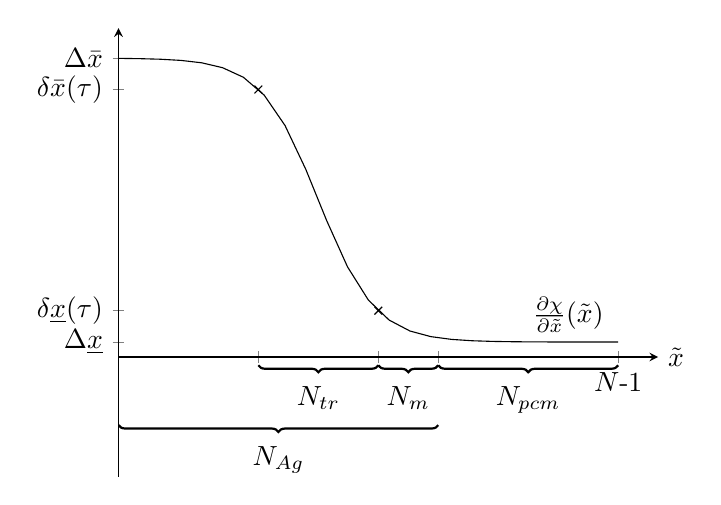
\begin{tikzpicture}
	\begin{axis}[
	axis x line = middle,
	axis y line = middle,
	xtick={7,13,16,25},
	ytick={0.05, 1., 0.155, 0.895},
	xticklabels={, , , $N\text{-}1$},
	yticklabels={$\Delta \underline{x}$, $\Delta \bar{x}$, $\delta \underline{x}(\tau)$, $\delta {\bar{x}}(\tau)$},
	xmin=0, xmax=27,
	ymin=-0.4, ymax=1.1,
	xlabel=$\tilde{x}$, xlabel style={at=(current axis.right of origin), anchor=west},
	]
	\addplot [domain=0:25] {(1 - 0.05) / (exp(0.7*(x-10))+1) + 0.05} node[pos=0.9, above, sloped] {$\frac{\partial \chi}{\partial \tilde{x}}(\tilde{x})$};
	
	\draw [thick,decoration={brace,mirror,raise=3pt},decorate] 
	(axis cs:16,0) --
	node[below=7pt] {$N_{pcm}$} 
	(axis cs:25,0);
	
	\draw [thick,decoration={brace,mirror,raise=3pt},decorate] 
	(axis cs:13,0) --
	node[below=7pt] {$N_{m}$} 
	(axis cs:16,0);
	
	\draw [thick,decoration={brace,mirror,raise=3pt},decorate] 
	(axis cs:7,0) --
	node[below=7pt] {$N_{tr}$} 
	(axis cs:13,0);
	
	\draw [thick,decoration={brace,mirror,raise=3pt},decorate] 
	(axis cs:0,-0.2) --
	node[below=7pt] {$N_{Ag}$} 
	(axis cs:16,-0.2);

	\addplot[only marks, mark=x, color=black] 
	table {7	0.895
	       13   0.155
	};	
	
	% L1
	\draw [loosely dashed] (0, 129.5) -- (70, 129.5);
	\draw [loosely dashed] (70, 40) -- (70, 129.5);	
	
	% L1 + L3
	\draw [loosely dashed] (0, 55.5) -- (130, 55.5);
	\draw [loosely dashed] (130, 40) -- (130, 55.5);	

	\draw [loosely dashed] (160, 20) -- (160, 40);	
	
	
	
	\end{axis}
	\end{tikzpicture}
	\caption{Illustrative mapping of the gridsize $\Delta x = \frac{\partial \chi}{\partial \tilde{x}}(\tilde{x})$ as a function of the computation grid $\tilde{x}$ (note: first discretization point at $\tilde{x}=0$). $N$, $N_{pcm}$, $N_m$ and $N_{tr}$ are the number of discretization points in total, within the PCM, margin and grid transition part. Start $\delta \bar{x}(\tau) := \Delta \underline{x} + (\Delta \bar{x} - \Delta \underline{x})\cdot \tau$  \ and end $\delta \underline{x}(\tau) := \Delta \underline{x} + (\Delta \bar{x} - \Delta \underline{x})\cdot(1-\tau)$ of the grid transition w.r.t. threshold $\tau$ are marked. Grid size lower and upper bound $\Delta \underline{x}$ and $\Delta \bar{x}$ used in \cref{eq:gridsize_definition}. \\
	Remark: Gridsize still changes noticeable outside transition zone here since threshold is set here to a very low value ${\tau=0.85}$ in order to illustrate how the gridsize construction works. In the numerical experiments ${\tau=0.999}$ was used.}
	\label{fig:grid_size}
\end{figure}


\subsection{Analytical solution of reference side}
\label{sec:analytical_solution}

%The measurement data for the residuum computation is given as a function dependent on the temperature at the reference crucible $T_{ref}^{\eta_i}$. Since we need to evaluate the solution of the heat equation (PCM side) at the corresponding time points $t_i$ it is necessary to calculate these.
%This is done by applying Newton's method on the heat equation's solution of the reference side which can be solved analytically as follows. \\

As the crucible of the reference side is empty there is only the silver plate with a constant temperature conductivity $\alpha_{Ag}=\frac{\lambda_{Ag}}{\rho_{Ag} \cdot c_{p,Ag}}$. The initial and boundary conditions are equal to the ones of the PCM side. Therefore the boundary value problem reads 

\begin{subequations}
	\begin{empheq}[box=\widefbox]{align}
		\frac{\partial T}{\partial t}(x,t) & - \alpha_{Ag} \cdot \frac{\partial^2 T}{\partial x^2}(x,t) = 0 & \ \forall \ x \in [0,L_{Ag}], \ \forall \ t \in [0,t_f]  \label{eq:analytical_soln_pde} \\
		T(0,t) & = T_0 + \beta \cdot t & \ \forall \ t \in [0,t_f] \label{eq:analytical_soln_bc_dirichlet} \\
		\frac{\partial T}{\partial x}(L_{Ag},t) & = 0 & \ \forall \ t \in [0,t_f] \label{eq:analytical_soln_bc_neumann}  \\
		T(x,0) & = T_0 &  \ \forall \ x \in [0,L_{Ag}]
	\end{empheq}
\end{subequations}

which can be solved analytically. The derivation is based on \cite{analytical_soln} chapter 5.6. If omitted in the following for legibility, it holds $x \in [0,L_{Ag}]$ and $t \in [0,t_f]$. \\
The first step is a separation ansatz of the solution function $T(x,t)$

\begin{align}
	{T}(x,t) =: & \ \bar{T}(x,t) + \Gamma(x,t) \\
	\bar{T}(x,t) =: & \ A(t) + B(t) \cdot x \label{eq:analytical_soln_bc_def}
\end{align}

The idea is that $\bar{T}(x,t)$ satisfies the boundary conditions and therefore the boundary value subproblem (see later \cref{eq:analytical_soln_gamma}) in $\Gamma(x,t)$ has homogeneous boundary conditions. \\
Inserting the boundary conditions and equating coefficients in $x$ gives

\begin{align}
	A(t) \stackrel{\eqref{eq:analytical_soln_bc_def}}{=} & \ \bar{T}(0,t)  \stackrel{\eqref{eq:analytical_soln_bc_dirichlet}}{=} T_0 + \beta \cdot t \\
	B(t) \stackrel{\eqref{eq:analytical_soln_bc_def}}{=} & \ \frac{\partial \bar{T}}{\partial x}(L_{Ag},t) \stackrel{\eqref{eq:analytical_soln_bc_neumann}}{=} 0 \\[2ex]
	\Rightarrow & \ \bar{T}(x,t) = T_0 + \beta \cdot t
\end{align}



By construction this leads to homogeneous boundary conditions of $\Gamma(x,t)$:

\begin{align}
	T(0,t) & = \bar{T}(0,t) + \Gamma(0,t) = T_0 + \beta \cdot t + \Gamma(0,t) \stackrel{\cref{eq:analytical_soln_bc_dirichlet}}{=} T_0 + \beta \cdot t \\
	 &\Rightarrow \Gamma(0,t) = 0 \\[2ex]
	\frac{\partial T}{\partial x}(L_{Ag},t) & = \underbrace{\frac{\partial \bar{T}}{\partial x}(L_{Ag},t)}_{= 0} + \frac{\partial \Gamma}{\partial x}(L_{Ag},t) \stackrel{\cref{eq:analytical_soln_bc_neumann}}{=} 0 \\
	 &\Rightarrow \frac{\partial \Gamma}{\partial x}(L_{Ag},t) = 0
\end{align}


Inserting $\bar{T}$ and $\Gamma$ into \cref{eq:analytical_soln_pde} gives

\begin{align}
	\frac{\partial \bar{T}}{\partial t} + \frac{\partial \Gamma}{\partial t} - \alpha_{Ag} \left[ \frac{\partial^2 \bar{T}}{\partial x^2} + \frac{\partial^2 \Gamma}{\partial x^2} \right] = 0
\end{align}
	

	
	
With $\frac{\partial \bar{T}}{\partial t} = \beta$, $\frac{\partial^2 \bar{T}}{\partial x^2} = 0$ and

\begin{align}
T(x,0) & = \underbrace{\bar{T}(x,0)}_{T_0} + \Gamma(x,0) = T_0 \\
& \Rightarrow \Gamma(x,0) = 0
\end{align}

this leads to the boundary value problem in $\Gamma(x,t)$

\begin{subequations}
	\begin{empheq}[box=\widefbox]{align}
		\frac{\partial \Gamma}{\partial t}(x,t) - \alpha_{Ag} \cdot \frac{\partial^2 \Gamma}{\partial x^2}(x,t) & =  \overbrace{-\beta}^{=: \bar{q}}   & \ \forall \ x \in [0,L_{Ag}], \ \forall \ t \in [0,t_f]  \label{eq:analytical_soln_pde_gamma} \\
		\Gamma(0,t) & = 0 & \ \forall \ t \in [0,t_f] \label{eq:analytical_soln_bc_neumann_gamma} \\
		\frac{\partial \Gamma}{\partial x}(L_{Ag},t) & = 0 &  \ \forall \ t \in [0,t_f] \label{eq:analytical_soln_bc_dirichlet_gamma}  \\
		\Gamma(x,0) & = 0 =: \bar{f} &  \ \forall \ x \in [0,L_{Ag}]
	\end{empheq}
	\label{eq:analytical_soln_gamma}
\end{subequations}


The homogeneous solution (i.e. $\bar{q}=0$) can be obtained by an separation ansatz of $\Gamma(x,t) =: \mathcal{T}(t) \cdot X(x)$. \Cref{eq:analytical_soln_pde_gamma} is then equivalent to

\begin{equation}
	\dot{\mathcal{T}} X = \alpha_{Ag} \mathcal{T} X'' \quad \Leftrightarrow \quad \frac{1}{\alpha_{Ag}} \frac{\dot{\mathcal{T}}}{\mathcal{T}} = \frac{X''}{X} = const =: - \lambda
\end{equation}


since the LHS $\sfrac{\dot{\mathcal{T}}}{{\mathcal{T}}}$ just depends on $t$ and the RHS $\sfrac{X''}{X}$ just depends on $x$. The constant defined ${-\lambda}$ is not to be mistaken with the physical quantity of the heat conductivity outside this section. 

The solution of the ordinary differential equation $X'' = - \lambda \cdot X$ is

\begin{equation}
	X(x) = c_1 \cdot \sin(\sqrt{\lambda} x) + c_2 \cdot \cos(\sqrt{\lambda} x)
\end{equation}

where $c_1$ and $c_2$ are determined by the boundary conditions $X(0) = 0$ and $X'(L_{Ag}) = 0$:

\begin{align}
	X(0) = c_2 \stackrel{!}{=} 0 \\
	X'(L_{Ag}) = \left. c_1 \sqrt{\lambda} \cos(\sqrt{\lambda} x) \right|_{x=L_{Ag}} = c_1 \sqrt{\lambda} \cos(\sqrt{\lambda} L_{Ag}) \stackrel{!}{=} 0 \\
	\Rightarrow \sqrt{\lambda_n} = \frac{(2n -1)\pi}{2 L_{Ag}} \qquad n=1,2,...
\end{align}

Note: The trivial solution $\sqrt{\lambda}=0$ leads to $X(x) = 0$ and is therefore omitted. \\
The eigenfunctions $X_n(x)$ are then given by

\begin{equation}
	\tilde{X}_n(x) = c_1 \cdot \sin\left(\frac{(2n -1)\pi}{2 L_{Ag}} \cdot x\right) =: c_1 \cdot X_n(x)
\end{equation}

In order to solve the non-homogeneous boundary value problem \cref{eq:analytical_soln_gamma}, $\Gamma$, $\bar{q}$ and $\bar{f}$ are expanded in a Fourier series with $X_n(x)$ as basis where $c_1$ is incorporated in the corresponding Fourier coefficients $\mathcal{T}_n(t)$, $\bar{q}_n(t)$ and $\bar{f}_n$:

\begin{subequations}
	\centering
	\begin{align}
		\Gamma(x,t) & = \sum_{n=1}^{\infty} \mathcal{T}_n(t) X_n(x) \\
		\bar{q}(x,t) & = \sum_{n=1}^{\infty} \bar{q}_n(t) X_n(x) \\
		\bar{f}(x) & = \sum_{n=1}^{\infty} \bar{f}_n X_n(x)
	\end{align}
\end{subequations}

The Fourier coefficients $\bar{q}_n(t)$ and $\bar{f}_n$ are then computed by

\begin{subequations}
	\begin{align}
		\bar{q}_n(t) & = \frac{\int_{0}^{L_{Ag}} \bar{q}(x,t) X_n(x) dx}{\int_{0}^{L_{Ag}} X_n^2(x) dx} \ \overbrace{=}^{\bar{q}=-\beta} \ - \frac{4 \beta}{\pi (2n - 1)} \\
		\bar{f}_n & = \frac{\int_{0}^{L_{Ag}} \bar{f}(x) X_n(x) dx}{\int_{0}^{L_{Ag}} X_n^2(x) dx} \ \underbrace{=}_{\bar{f}=0} 0
	\end{align}
\end{subequations}

Inserting this into \cref{eq:analytical_soln_pde_gamma} gives us

\begin{align*}
	\sum_{n=1}^{\infty} \dot{\mathcal{T}}_n(t) X_n(x) - \alpha_{Ag} \sum_{n=1}^{\infty} \mathcal{T}_n(t) X_n''(x) = \sum_{n=1}^{\infty} \bar{q}_n(t) X_n(x) \nonumber \\
	\stackrel{X'' = - \lambda X}{\Leftrightarrow} \ \ \sum_{n=1}^{\infty} \dot{\mathcal{T}}_n(t) X_n(x) + \alpha_{Ag} \sum_{n=1}^{\infty} \lambda_n \mathcal{T}_n(t) X_n(x) = \sum_{n=1}^{\infty} \bar{q}_n(t) X_n(x)
\end{align*}

With equating the coefficients in $X_n$ we get the inhomogeneous ordinary differential equation (ODE)

\begin{equation}
	\dot{\mathcal{T}_n}(t) + \alpha_{Ag} \lambda_n \mathcal{T}_n(t) = \bar{q}_n(t)
	\label{eq:analytical_soln_inhomo_ode}
\end{equation}

where the solution of the homogeneous part (i.e. $\bar{q}_n(t) = 0$) is

\begin{equation}
	\mathcal{T}_n^h(t) = A_n \cdot e^{-\alpha_{Ag} \lambda_n t}
\end{equation}

Applying the method of variation of constants by setting $A_n = A_n(t)$ and inserting in \cref{eq:analytical_soln_inhomo_ode} gives after cancellation and reordering

\begin{align}
	\dot{A_n}(t) & = \bar{q}_n(t) \cdot e^{\alpha_{Ag} \lambda_n t} = -\frac{4 \beta}{\pi (2n - 1)} e^{\alpha_{Ag} \lambda_n t} \\
	\Rightarrow A_n(t) & = \int_{0}^{t} -\frac{4 \beta}{\pi (2n - 1)} e^{\alpha_{Ag} \lambda_n \tau} d \tau + A_{n,c} \\
	& = -\frac{4 \beta}{\pi (2n - 1)} \frac{1}{\alpha_{Ag} \lambda_n} \left[ e^{\alpha_{Ag} \lambda_n t} - 1 \right] + A_{n,c}
\end{align}

where $A_{n,c}$ is the constant part from integration since no initial value has been applied yet, it will be determined in the following.

The solution of the inhomogeneous ODE \cref{eq:analytical_soln_inhomo_ode} then is
\begin{align}
	\mathcal{T}_n(t) & = A_n(t) \cdot e^{-\alpha_{Ag} \lambda_n t}  \\
	& = -\frac{4 \beta}{\pi (2n - 1)} \frac{1}{\alpha_{Ag} \lambda_n} \left[1 - e^{-\alpha_{Ag} \lambda_n t} \right] + A_{n,c} e^{- \alpha_{Ag} \lambda_n t} \nonumber
\end{align}

The remaining unknown $A_{n,c}$ is determined by considering the Fourier series of the starting condition

\begin{equation}
	\Gamma(x,0) = \sum_{n=1}^{\infty} \mathcal{T}_n(0) X_n(x) = \sum_{n=1}^{\infty} \bar{f}_n X_n(x) = \bar{f}(x)
\end{equation}

From $\mathcal{T}_n(0) = A_{n,c}$, $\bar{f}_n=0$ and again equating the coefficients it follows that

\begin{equation}
	A_{n,c} = 0
\end{equation}

Finally the solution of the boundary value problem \cref{eq:analytical_soln_pde} of the reference side reads as

\begin{align}
	& \ \ T(x,t) = \bar{T}(x,t) + \Gamma(x,t) \nonumber \\
	\Leftrightarrow \ \ & T(x,t) = T_0 + \beta \cdot t + \sum_{n=1}^{\infty} \mathcal{T}_n(t) X_n(x) \nonumber \\[1ex]
	\Leftrightarrow \ \ & \raalign{}{T(x,t) = T_0 + \beta \cdot t - \sum_{n=1}^{\infty} \left\{ \frac{4 \beta}{\pi (2n - 1)} \frac{1}{\alpha_{Ag} \cdot \lambda_n} \left[ 1 - e^{- \alpha_{Ag} \lambda_n t} \right] \cdot \sin(\sqrt{\lambda_n} \cdot x) \right\}} \label{eq:analytical_soln_final_formula}
\end{align}


\newpage
\section{Parameter estimation of specific heat capacity $c_p$}
\label{sec:parameter_estimation_applied}

The measuring process simulation, described in \cref{sec:simulation_of_DSC} is embedded in this section into the parameter estimation of the specific heat capacity $c_p(T)$ where a nonlinear least squares problem has to be solved. The corresponding numerical experiments are elucidated in \cref{sec:numerical_experiments}.
As we want to estimate a function, $c_p(T)$ has been parametrized.
Those parametrization used in this thesis will be introduced in the following.


\subsection{Parametrizations of $c_p$}
\label{sec:parametrizations}

In this thesis the following three parametrizations for the specific heat capacity $c_p(T)$ has been used.

\subsubsection{NURBS}
\label{sec:nurbs}
In preliminary computations, we used Non-Uniform Rational B-Splines (NURBS), see e.g. \cite{the_NURBS_book}. The generated curve $C(u) = \begin{pmatrix}
C^x(u), C^y(u) \end{pmatrix}^T \in \mathbb{R}^2$ is defined by

\begin{equation}
	C(u) = \frac{\sum_{i=0}^{n} N_{i,p}(u) \omega_i P_i }{\sum_{i=0}^{n} N_{i,p}(u) \omega_i} \qquad a \le u \le b
\end{equation}

where $P_i = \begin{pmatrix}
P_i^x, P_i^y \end{pmatrix}^T \in \mathbb{R}^2$ are called control points, $\omega_i$ are weights for each control point. Here we restrict ourselves to $\omega_i \ge 0$ where at least one weight has to be larger than zero.
B-Spline basis functions $N_{i,p}(u)$ are defined recursively by

\begin{align}
	N_{i,p}(u) = & \frac{u - u_i}{u_{i+p} - u_i} N_{i,p-1}(u) + \frac{u_{i+p+1} - u}{u_{i+p+1} - u_{i+1}} N_{i+1,p-1}(u) \label{eq:NURBS_basis_polynomial} \\[1ex]
	N_{i,0} = &
	\begin{cases}
		1 \quad \text{if } u_i \le u < u_{i+1} \\
		0 \quad \text{otherwise}
	\end{cases} \nonumber
\end{align}

where $u_i$ are the elements of the knot vector

\begin{equation}
	U = (u_0,...,u_m)^T =
	(\underbrace{a,...,a}_{p+1},u_{p+1},...,u_{m-p-1},\underbrace{b,...,b}_{p+1})^T
	\label{eq:NURBS_knot_vector}
\end{equation}

With this formulation there are $n+1$ control points, $p$ is the order of the basis functions and the order of the resulting curve is defined by $p+1$. It holds ${m=n+p+1}$. The interval $[a,b]$ is arbitrary in the sense that with the knot vector \cref{eq:NURBS_knot_vector} it holds that $C(u=a)=P_0$, $C(u=b)=P_n$ and $u \in (a,b)$ are points between. \\

In our experimental setup we used NURBS of order $4$, i.e. $p=3$. It was set $a=0$ and $b=1$ such that $u \in [0,1]$ and the knot vector reads
\begin{equation}
	U = (0,0,0,0,\frac{1}{n-p+1},\frac{2}{n-p+1},...,\frac{n-p}{n-p+1},1,1,1,1)^T 
\end{equation}
All control points contribute equally such that $\omega_i=1 \ \forall \ i$. 
%With these settings it holds that $C(u) \in \mathcal{C}^2$.

Since $C(u)$ is a parametrized curve we get a function $c_p(T)$ by using $C^x(u)$ as the domain of definition (temperature) and $C^y(u)$ as the co-domain ($c_p$). Evaluating $C(u)$ on an appropriate fine grid for values of $u$ and subsequently piecewise linear interpolation gives the wanted quantity $c_p(T)$, although not differentiable then.
The x-coordinates of the control points were fixed on a predefined grid with $P_i^x < P_{i+1}^x$ to get a well-defined function.
As optimization variables we used the corresponding y-coordinates $P_i^y$. \\
The corresponding numerical experiments with this parametrization are found in \cref{sec:param_estim_NURBS}. \\

As we switched for the derivative computation with respect to the optimization variables from finite differences to IND, implementation problems occurred with the case structure of \cref{eq:NURBS_basis_polynomial}. The evaluation of piecewise polynomials leads to a case structure as well. Those are supported by SolvIND only in a very limited way and not appropriate to handle these two complex case structures. Therefore the two following parametrizations has been used with IND.


\subsubsection{Linear combination of Gaussian functions}
\label{sec:parametrization_Gausse}

%As we switched for the derivative computation with respect to the optimization variables from finite differences to IND using the software SolvIND, implementation problems with NURBS occurred. 
%The case structure of the basis polynomial \cref{eq:NURBS_basis_polynomial} conducts to switch the RHS of the differential equation. This is only supported by the $condassign(a,b,c,d)$ function which assigns $a=c$ if $b>0$ and $a=d$ else. Additionally to $N_{i,0}$ the denominators need this $condassign$ command in order to check for a division by zero. 
%Furthermore the piecewise interpolation of the resulting curve $C(u)$ could be realized as well with the $condassign$ command but in total this leads to a lot of unnecessary numerical operations and makes the program quite complex. \\

An alternative flexible parametrization is a linear combination of Gaussian functions which is stated in \cref{eq:parametrization_linear_comb_Gauss}. For each Gaussian, there are three optimization variables: Amplitude $A_i$, a shift in the $T$-axis $T_{\text{offset}_i}$ and the variance $\var_i$. Additionally there is a linear and constant part with variables $m$ and $b$. So in total there are $3 \cdot n_{\text{Gauss}} + 2$ optimization variables. 

\begin{equation}
c_p(T) = \sum_{i=1}^{n_{\text{Gauss}}} A_i \exp\left(- \frac{(T - T_{\text{offset}_i})^2}{{\var}_i}\right) + m \cdot T + b
\label{eq:parametrization_linear_comb_Gauss}
\end{equation} \\

An exemplary $c_p(T)$ function generated by this parametrization is shown in \cref{fig:parametrization_example_linear_comb_gauss}.


\begin{figure}[H]
	\centering
	\includegraphics[width=0.75\textwidth]{/home/argo/masterarbeit/thesis/images/c_p_example.png}
	\caption{Example of 5 Gaussians reconstructing a Fraser-Suzuki shaped peak (see \cref{sec:parametrization_FS}). Each individual Gaussian and  the resulting function $c_p(T)$ is plotted where the linear and constant part is added each time for better illustration.}
	\label{fig:parametrization_example_linear_comb_gauss}
\end{figure}



\subsubsection{Fraser-Suzuki peak}
\label{sec:parametrization_FS}

A parametrization used frequently for chromatography and spectroscopy distributions with fewer degrees of freedom is the Fraser-Suzuki peak \cite{fraser_suzuki_1} \cite{fraser_suzuki_many_fcts}

\begin{align}
	c_p(T) =
	\begin{cases}
		h \cdot \exp \left\{ - \frac{\ln(r)}{\ln(s_r)^2} \cdot \left[ \ln\left( 1 + (T-z) \cdot \frac{s_r^2 - 1}{w_r \cdot s_r} \right) \right]^2 \right\} + m \cdot T + b \ & \text{for } \ T < z - \frac{w_r \cdot s_r}{s_r^2 - 1} \\
		m \cdot T + b \ & \ \text{else}
	\end{cases}
	\label{eq:fraser_suzuki}
\end{align}

where $h$, $r$, $s_r$, $w_r$ and $z$ are the parameters of Fraser-Suzuki. In order to keep the argument of the logarithm positive it must hold $r > 0$, $w_r > 0$ and $s_r > 0$. Besides, at $s_r = 1$ the denominator with $\ln(s_r)^2$ becomes zero such that the condition $0 < s_r < 1$ is appropriate. Furthermore, the parameters for linear part $m$ and constant part $b$ were added to model a linear base line. An example is given in \cref{fig:parametrization_example_fraser_suzuki}.

\begin{figure}[H]
	\centering
	\includegraphics[width=0.8\textwidth]{/home/argo/masterarbeit/thesis/images/fraser_suzuki_example.png}
	\caption{Example of Fraser-Suzuki peak with $h=10$, $r=2$, $wr=5$, $sr=0.3$, $z=130$, $m=0.003$, $b=2$.}
	\label{fig:parametrization_example_fraser_suzuki}
\end{figure}











\newpage
\subsection{Optimization problem}
\label{sec:optimization_problem}
In order to perform the parameter estimation to determine $c_p(T)$ we need to solve the nonlinear least squares problem

\begin{align}
	\min_{p_{c_p}} \ & \sum_{i=1}^{n_{mp}} \left(  \varPhi_{q}^{pcm,in}(T(t_i;T_0,p_{c_p})) - \varPhi_q^{\eta_i} \right)^2 \label{eq:parameter_estimation_least_squares_problem} \\
	s.t. \ & \quad \  \dot{T} = f(T,t;p_{c_p}) \nonumber \\
	& T(0) = T_0 \nonumber \\
	& \ \ \bar{p}_{c_p} \ge p_{c_p} \ge \underline{p}_{c_p} \nonumber
\end{align}

where $p_{c_p} \in \mathbb{R}^{n_p}$ are the optimization variables, parametrizing the specific heat capacity $c_p(T)$, $n_{{mp}}$ is the number of measurement points, $\varPhi_{q}^{pcm,in}$ is the simulated heat flux into the PCM calculated from the solution $T(t_i;T_0,p_{c_p}) \in \mathbb{R}^N$ of the discretized heat equation and $\varPhi_q^{\eta_i}$ is the heat flux measurement value at measurement time $t_i$. 
Note here that the same measurement variance $\sigma^2$ is assumed for all measurement values and it was set implicitly to $\sigma^2=1$.
The model $\dot{T} = f(T,t;p_{c_p})$ with $T(0) = T_0$ is equivalent to the initial value problem \cref{eq:heat_equation_discretized} of solving the discretized heat equation. Lower and upper bounds for the optimization variables are set by $\underline{p}_{c_p}$ and $\bar{p}_{c_p}$, respectively to guarantee that the model can be evaluated\footnote{E.g., to prevent division by zero in a evaluation of the parametrized function $c_p(T)$.}.
This least squares problem is of the form of \cref{eq:param_estimation_definition}, which has been discussed in \cref{sec:parameter_estimation_theory}.

\subsubsection{Mapping measured reference temperature $T_{ref}^{\eta_i}$ to measurement times $t_i$}

The measurement data is given as $\varPhi_q^{\eta_i}(T_{ref}^{\eta_i})$ where $T_{ref}^{\eta_i}$ is the temperature at the reference crucible at measurement time $t_i$. Since we need to pass these times $t_i$ to the differential equation solver for the evaluation of the temperature and sensitivities we obtain them by solving the nonlinear equation 

\begin{align}
	T_{ref}^{\eta_i} - T_{ref}^{sim}(t_i) = 0 \quad \forall \ i = 1,2,...,n_{mp}
	\label{eq:measurement_time_computation}
\end{align}

using Newton's method where $T_{ref}^{sim}(t)$ is the analytical solution of the heat equation on the reference side \cref{eq:analytical_soln_final_formula}. An illustration is given in \cref{fig:obtaining_measurement_times}. The analytical solution (\cref{sec:analytical_solution}, \cref{eq:analytical_soln_final_formula}) can be applied here since on the reference side the material properties (pure silver) are constant. The time at which the furnace temperature $T_{furnace}$ is equal to the measured reference crucible temperature $T_{ref}^{\eta_i}$ has been used as initial value of the measurement time $t_{i,init}$ for Newton's method. 

\begin{align}
	T_{ref}^{\eta_i} \stackrel{!}{=} & T_{furnace}(t_{i,init}) = T_0 + \beta \cdot t_{i,init} \nonumber \\
	& \Leftrightarrow \ t_{i,init} = \frac{T_{ref}^{\eta_i} - T_0}{\beta}
\end{align}

This is reasonable since the difference between these two temperatures is very small (note that in \cref{fig:obtaining_measurement_times} the difference is exaggerated for a better illustration of the principle). \\


\begin{figure}[H]
	\centering
	\begin{tikzpicture}
	\begin{axis}[domain=0:65,
	samples=100,
	xmin=0, xmax=70,
	ymin=0.,	 
	axis lines=left,
	xtick={40},
	xticklabels={$t_i$},
	ytick={0.7, 3.7},
	yticklabels={$T_0$, $T_{ref}^{\eta_i}$},
	xlabel=$time$, xlabel style={at=(current axis.right of origin), anchor=west},
	ylabel=\empty
	]
	
	\addplot+[color=black, mark=none] {0.7 + 0.1*x}
	node[pos=0.87, above, sloped] {$T_{{furnace}}$};
	
	\addplot+[color=black, mark=none] {0.7 + 0.1*x - (1 - exp(-0.11*x)}
	node[pos=0.95, below, sloped] {$T_{{ref}}^{{sim}}$};
	
	\addplot[only marks, mark=x, color=black] 
	table {40 3.7
	};	
	
	\draw [loosely dashed] (0, 370) -- (400, 370);
	\draw [loosely dashed] (400, 0) -- (400, 370);	
	
	\end{axis}
	\end{tikzpicture}
%	\caption{Illustration how the measurement times $t_i$ were obtained. Given the measured temperatures $T_{ref}^{\eta_i}$ and the simulated temperature $T_{ref}^{sim}(t)$ at the reference crucible. Then $\{ t_i \}_{i=1,...n_{mp}}$ are computed via Newton's method which are used in the parameter estimation least squares problem \cref{eq:parameter_estimation_least_squares_problem}.}
	\caption{Temporal development of the temperature at the reference crucible $T_{ref}^{sim}$ for a linear heating program of the furnace temperature $T_{furnace}$. Measurement time $t_i$ at which reference crucible has temperature $T_{ref}^{\eta_i}$ is computed by applying Newton's method on \cref{eq:measurement_time_computation}. The measurement times $t_i$ are used in the parameter estimation least squares problem \cref{eq:parameter_estimation_least_squares_problem}.}
	\label{fig:obtaining_measurement_times}
\end{figure}

\subsubsection{Heat flux residuum and optimization Jacobian computation}

For the optimization process using Gauss-Newton method (see \cref{sec:Gauss_Newton}) we define the residuum vector 

\begin{equation}
	F_1(p_{c_p}) :=
	\begin{pmatrix}
		\varPhi_{q}^{pcm,in}(T(t_1;T_0,p_{c_p})) - \varPhi_q^{\eta_1} \\
		\textcolor{white}{} \\
		\vdots \\
		\textcolor{white}{} \\
		\varPhi_{q}^{pcm,in}(T(t_{n_{mp}};T_0,p_{c_p})) - \varPhi_q^{\eta_{n_{mp}}}
	\end{pmatrix}
\end{equation}

whose squared euclidean norm $|| \cdot ||_2^2$ will be minimized. 
By applying the chain rule we get its Jacobian

\begin{equation}
	J_1(p_{c_p}) := \frac{\partial F_1}{\partial p_{c_p}} =
	\begin{pmatrix}
		\frac{\partial \varPhi_{q}^{pcm,in}}{\partial T}(T(t_1)) \cdot \frac{\partial T}{\partial p_{c_p}}(t_1) \\
		\textcolor{white}{} \\
		\vdots \\
		\textcolor{white}{} \\
		\frac{\partial \varPhi_{q}^{pcm,in}}{\partial T}(T(t_{n_{mp}})) \cdot \frac{\partial T}{\partial p_{c_p}}(t_{n_{mp}}) \\
	\end{pmatrix}
	\label{eq:optimization_jacobian}
\end{equation}

with

\begin{align}
	\frac{\partial \varPhi_{q}^{pcm,in}}{\partial T}(T(t_i)) = - \frac{\lambda_{pcm} \ m_{pcm}}{N_{pcm} \ \rho_{pcm} \ (\Delta x_{N_{Ag}})^2} \cdot
	\left(\begin{array}{cccccccc}
	\undermat{N_{Ag}}{0 & ... & 0} & -1 & +1 & \undermat{N_{pcm}-2}{0 & ... & 0}
	\end{array}\right) \\[2ex]
	\forall \ i = 1,...,n_{mp} \nonumber
\end{align}

using \cref{eq:heat_flux_computation_final}. The non-zero entries are in column $N_{Ag+1}$ and $N_{Ag}+2$ (since first discretized temperature is $T^0$). 
The sensitivities $\frac{\partial T}{\partial p_{c_p}}(t_i) \in \mathbb{R}^{N \times n_p}$ can be computed by the methods described in \cref{sec:Automatic_diff_IND_theory}. 


\newpage
\section{Numerical experiments and results}
\label{sec:numerical_experiments}


All conducted numerical experiments involve the following subproblems: The numerical integration where we solve \cref{eq:heat_equation_discretized} gives us the temperature vector $T = \begin{pmatrix} T^0 & ... & T^{N-1}  \end{pmatrix}^T$ and sensitivities $\frac{\partial T}{\partial p}$. This was accomplished with the numerical integrator DAESOL-II embedded in SolvIND. The integration tolerance was set to $10^{-7}$ except in \cref{sec:param_estimation_fs}.
The sensitivities were obtained in forward mode. Theoretically adjoint mode is computationally cheaper since we just need two adjoint directions $T^{N_{Ag}}$ and $T^{N_{Ag}+1}$ compared to $n_p$ directions in forward mode. But in practice it turned out that the computation is faster using the forward mode.
The heat flux $\varPhi_q^{pcm,in}$ is then computed with \cref{eq:heat_flux_computation_final} and the optimization Jacobian $J_1(p_{c_p})$ with \cref{eq:optimization_jacobian}. Usual choice for PCM discretization points was set to $N_{pcm}=50$ as the heat flux approximation error is then negligible. The parameter estimation is performed by solving the least squares problem \cref{eq:parameter_estimation_least_squares_problem} on the one hand with the Matlab routine $lsqnonlin$ which uses a trust-region method and Gauss-Newton directions based on interior-reflective Newton method described in \cite{lsqnonlin_alg1} and \cite{lsqnonlin_alg2}. Later then, a self written Gauss-Newton solver has been used (\cref{alg:Gauss_Newton_unconstrained}).
When solving the reference side with the analytical solution \cref{eq:analytical_soln_final_formula} we stopped the actually infinite sum after $100$ summands which is definitively sufficient, since the $n$'th summand is proportional to $n^{-3}$. \\

The constant material properties used throughout are shown in \cref{tab:const_material_properties}.

\begin{table}[H]
	\centering
	\begin{tabular}{| c | c | c | c |} \hline
		& $c_p \ [\frac{mJ}{mg \ K}]$ & $\rho \ [\frac{mg}{mm^3}]$ & $\lambda \ [\frac{mW}{mm \ K}]$ \\ \hline
		Silver (Ag) & $0.235$ & $10.49$ & $430$ \\
		PCM & ---$^*$ & $0.85$ & $0.96$ \\ \hline
	\end{tabular}
	\caption{Material properties for specific heat capacity $c_p$, mass density $\rho$ and heat conductivity $\lambda$ used in numerical experiments. $^*$ Specific heat capacity of PCM is temperature dependent and parametrized, see \cref{sec:parametrizations}.}
	\label{tab:const_material_properties}
\end{table}

The initial temperature (see \cref{eq:heat_equation_discretized}) was set to $T_0=10^\circ C$ and the simulation stopped for the furnace temperature $T^0(t_f)=200^\circ C$ such that the phase transition is finished entirely. \\

%Except for the forward simulation with an equidistant grid as reference for the error analysis of different spatial grids, all experiments have been done on my laptop using Linux Ubuntu Mate, 2 Cores Intel(R) Core(TM) i3-4100M CPU @ 2.50GHz and 8GB RAM. Former was computed on the IWR-Compute Server Quadxeon2 (4 x Dual Core E7220 2.93 GHz, 256 GB RAM).

All experiments have been done on my laptop using Linux Ubuntu Mate, 2 Cores Intel(R) Core(TM) i3-4100M CPU @ 2.50GHz and 8GB RAM. 


\subsection{Smearing effect on simulated heat flux for different heat rates}
The first basic numerical experiment shows that our mathematical model is capable of reproducing heat fluxes exhibiting the smearing effect similar to those measured (see \cref{sec:smearing_problem}). This was achieved by a forward simulation, i.e. solving \cref{eq:heat_equation_discretized} for several different heat rates using the same specific heat capacity (see \cref{fig:smearing_effect_c_p}) each time. \\
The resulting heat fluxes for all heat rates from the forward simulation can be seen in \cref{fig:smearing_effect_simulation_heat_flux}. They exhibit a widening of the peak and a shift of the maximum to higher temperatures for increasing heat rates similar to the measured heat fluxes shown in \cref{fig:smearing_effect_measurement_heat_flux}. This forms the basis of reproducing the heat flux measurement values by performing a parameter estimation in the following numerical experiments in order to obtain the specific heat capacity.\\



\begin{figure}[H]
	\centering
	\begin{subfigure}{0.9\textwidth}
		\centering
		\includegraphics[width=0.5\textwidth]{/home/argo/masterarbeit/thesis/images/smearing_effect_simulation_c_p.png}
		\caption{}
		\label{fig:smearing_effect_c_p}
	\end{subfigure} \\
	\begin{subfigure}{0.49\textwidth}
		\includegraphics[width=1.\textwidth]{/home/argo/masterarbeit/thesis/images/heat_flux_measurement.png}
		\caption{}
		\label{fig:smearing_effect_measurement_heat_flux}
	\end{subfigure}
	\begin{subfigure}{0.49\textwidth}
		\includegraphics[width=1.\textwidth]{/home/argo/masterarbeit/thesis/images/smearing_effect_simulation_heat_fluxes_zoom.png}
		\caption{}
		\label{fig:smearing_effect_simulation_heat_flux}
	\end{subfigure}
	\caption{(a) Used specific heat capacity for all heat rates. Parametrization is Fraser-Suzuki (\cref{eq:fraser_suzuki}) with $h=10$, $r=2$, $wr=5$, $sr=0.3$, $z=130$, $m=0.003$ and $b=2$. (b) Heat flux measurement values for specified heat rates. (c) Heat flux from simulation for specified heat rates. Widening of the peak and shift of maximum position visible analogously to measurement values. \\
	Cf. smearing problem in \cref{sec:smearing_problem}.}
\end{figure}



\subsection{Preliminary parameter estimation using NURBS parametrization and optimization jacobian computed via finite differences}
\label{sec:param_estim_NURBS}

For the first attempt of estimating $c_p(T)$  we used the NURBS parametrization (see \cref{sec:nurbs}). In total we used 33 control points where the y-coordinates ($\hat{=}$ $c_p$) are optimization variables and the x-coordinates ($\hat{=}$ $T$) were fixed to 

\begin{equation}
	P^x = (0, 30, 60, 90, 100, 102, 104, ..., 148, 150, 160, 180, 200)
\end{equation}

such that the peak has enough degrees of freedom for temperatures $T \in [100, 150]$. \\
Due to the early working state we used the matlab routines $ode15s$ for integration and $lsqnonlin$ to solve the least squares problem where the Jacobian was computed via external numerical differentiation. The integration tolerance was set here to $10^{-7}$ as well. Moreover, material properties of Constantan were used instead of silver for the heat transport plate from furnace to PCM. In particular these are $c_{p,Const}=0.41\frac{mJ}{mg \ K}$, $\rho_{Const}=10.49\frac{mg}{mm^3}$ and $\lambda_{Const}=23\frac{mW}{mm \ K}$. Minimizing the heat flux residuum worked best in this setting for $L_{Const}=15mm$ (instead of $L_{Ag}$ here) and $L_{pcm}=0.5mm$. \\
The results after optimizing, using the measurement data of heat rate $\beta = 10 \frac{K}{min}$, are shown in \cref{fig:NURBS_results}. As one can see it was possible to minimize the heat flux residuum quite well aside from some oscillations which have their origin in $c_p(T)$. 
Beside the oscillations, there is one major difference in the peak shape of the specific heat capacity from what we would expect. That is, after the peak a temporary decrease is followed by a big slope.
Finally $lsqnonlin$ gives us the approximation of the used Jacobian $J_1(p_{c_p})$ at the end of the optimization process which was computed internally via finite differences, see \cref{fig:NURBS_results}. Since in our NURBS parametrization the y-coordinates of the control points are free optimization variables and the locality property of those, the x-axis of these Jacobian plots was set being the x-coordinates ($\hat{=}$ temperature) of the control points. This way there is a direct connection between $J_1(p_{c_p})$ and which zone of $c_p(T)$ it affects. The y-axis was labeled using the reference crucible temperature $T_{ref}$ since the heat flux measurement values are given as a function of those, analog to the heat flux plot.
Two things are worth mentioning. First there is an increase of several orders of magnitude for areas of $c_p(T)$ up to temperatures of $100^\circ C$ and $T_{ref}$ above $110^\circ C$ during phase transition. Interestingly the specific heat capacity's oscillations occur in a zone of low sensitivities which explains why $lsqnonlin$ does not improve here further. 
Secondly considering the zone of increased magnitude in detail (see \cref{fig:NURBS_results}d) one recognize sign switching oscillations where continuity is expected. This is a strong indication that the approximation of $J_1(p_{c_p})$ via finite differences is of poor quality and not reliable why we switch to internal numerical differentiation later. \\
The optimization took in this case about 40 minutes on my laptop and stopped because the norm of step was below the tolerance $10^{-6}$.


\begin{figure}[H]
	\begin{subfigure}{0.49\textwidth}
		\includegraphics[width=1.\textwidth]{/home/argo/masterarbeit/thesis/images/NURBS_heat_flux.png}
		\caption{}
	\end{subfigure}
	\begin{subfigure}{0.49\textwidth}
		\includegraphics[width=1.\textwidth]{/home/argo/masterarbeit/thesis/images/NURBS_c_p(T).png}
		\caption{}
	\end{subfigure}
	\begin{subfigure}{0.49\textwidth}
		\hspace{0.1cm}
		\includegraphics[width=1.\textwidth]{/home/argo/masterarbeit/thesis/images/NURBS_jac2.png}
		\caption{}
	\end{subfigure}
	\begin{subfigure}{0.49\textwidth}
		\hspace{0.4cm}
		\includegraphics[width=1.\textwidth]{/home/argo/masterarbeit/thesis/images/NURBS_jac_zoom2.png}
		\caption{}
	\end{subfigure}
	\caption{(a) Heat flux into PCM $\varPhi_q^{pcm,in}$ measurement values (dashed red), simulation (blue) and corresponding residuum (yellow). (b) Specific heat capacity $c_p(T)$ obtained by parameter estimation. (c) Approximated Jacobian $J_1(p_{c_p})$, note the big differences in order of magnitude. (d) Zoomed view of oscillations in approximated $J_1(p_{c_p})$. \\
	Explanation of the Jacobian axes labelings in text above.}
	\label{fig:NURBS_results}
\end{figure}




\subsection{Error analysis with respect to integration tolerance}
In this section we quantify the occurring numerical errors due to the used integration tolerance in order to ensure that this does not influence the results significantly. The same specific heat capacity as in \cref{fig:smearing_effect_c_p} has been used. \\
From here on the numerical integrator DAESOL-II within the SolvIND Suite and the material properties of silver for the silver plate were used for all upcoming numerical experiments. \\
The relative error computed by

\begin{align}
	|Relative \ error| = \left|1 - \frac{T^{N_{Ag}-1}_{tol=10^-7}}{T^{N_{Ag}-1}_{tol=10^-8}} \right|,
	\label{eq:relErr_integration_tolerance}
\end{align}

comparing integration tolerances $10^{-7}$ and $10^{-8}$  is shown in \cref{fig:integration_tolerance_error}.
The temperature at the last discretization point of the silver plate $T^{N_{Ag-1}}$ was evaluated for all measurement time points which equates a temperature at the reference crucible $T_{ref}$. 
The maximum relative error $1.7 \cdot 10^{-6}$ occurs approximately at the PCM's phase transition. 
From the magnitude we can conclude that an integration tolerance of $10^{-7}$ is sufficient. \\


\begin{figure}[H]
	\centering
	\includegraphics[width=0.75\textwidth]{/home/argo/masterarbeit/thesis/images/integration_tolerance_relErr.png}
	\caption{Relative error of temperature $T^{N_{Ag}-1}$ dependent on reference crucible temperature $T_{ref}$ computed by \cref{eq:relErr_integration_tolerance} for integration tolerances $10^{-7}$ and $10^{-8}$. Maximum value is $1.7 \cdot 10^{-6}$.}
	\label{fig:integration_tolerance_error}
\end{figure}


\subsection{Error analysis with respect to spatial discretization grid}
Next we compare several configurations of the spatial discretization grid (see \cref{sec:spatial_discretization_grid} for grid construction) with an equidistant reference grid with $\Delta x = \frac{L_{pcm}}{N_{pcm}}$ everywhere. The used physical lengths $L_{Ag}=40mm$ and $L_{pcm}=0.1mm$ where the optimization worked best and a sufficiently large number of discretization points within the PCM such that the heat flux approximation is adequate, results in a huge number of total discretization points in an equidistant grid. E.g. with $N_{pcm}=50$ the total number of discretization points would be $N=20,050$ which is not practical in the optimization process. Therefore we compute the relative error

\begin{equation}
	| \text{Relative error}_i| = \left| 1 - \frac{T_{{grid}_i}^{N_{Ag}-1}(T_{ref})}{T_{eq}^{N_{Ag}-1}(T_{ref})} \right|
	\label{eq:relErr_grid}
\end{equation}

where $T_{grid_i}^{N_{Ag}-1}$ is the temperature using grid $i$ and $T_{eq}^{N_{Ag}-1}$ is the temperature from the reference equidistant grid using $N_{pcm}=50$ and $N_{Ag}=20,000$. Both temperatures are evaluated at the silver plate's last discretization point since this equates to the same physical coordinate $x=L_{Ag}$ by construction in all grids. 
We set $n_m=0.01$ and $t=0.999$ for all experiments in order to guarantee that the transition of the grid size is finished sufficiently once the PCM starts which is necessary for the heat flux approximation. The same specific heat capacity as in \cref{fig:smearing_effect_c_p} has been used. \\

\subsubsection{Varying total number of discretization points $N$}
In the first set of tests we varied the total number of discretization points $N$ while fixing $n_{pcm}=0.2$ and $n_{tr}=0.1$. The results are shown in \cref{fig:grid_mod_N} where in all upcoming cases (a) shows the grid size $\Delta x = \frac{\partial \chi}{\partial \tilde{x}}(\tilde{x})$ as a function of the computation grid $\tilde{x}$ (the y-axis is logarithmic since differences in the minimum gridsize $\Delta x$ are better recognizable then) and (b) maps the corresponding relative error computed by \cref{eq:relErr_grid}. In all cases the error increases during the phase transition at the reference crucible temperature of about $130^{\circ} C$ where the maximum is reached for the least amount of tested discretization points $N=200$ with $|\text{Relative error|}=1.5 \cdot 10^{-5}$. Surprisingly the error for $N > 1000$ increases again but in all tested cases the relative error has an order of magnitude lower equal than $10^{-5}$. 


\begin{figure}[H]
	\begin{subfigure}{0.49\textwidth}
		\includegraphics[width=1.\textwidth]{/home/argo/masterarbeit/simulationen-data/grid_error/mod_N_gridsize.png}
		\caption{}
		\label{fig:gridsize_mod_N}
	\end{subfigure}
	\begin{subfigure}{0.49\textwidth}
		\includegraphics[width=1.\textwidth]{/home/argo/masterarbeit/simulationen-data/grid_error/mod_N_relErr.png}
		\caption{}
		\label{fig:grid_relErr_mod_N}
	\end{subfigure}
	\caption{(a) Grid size $\Delta x(\tilde{x})$ and (b) relative error computed by \cref{eq:relErr_grid} for fixed $n_{tr}=0.1$ and $n_{pcm}=0.2$ while varying total number of discretization points $N$. \\
	Cf. grid construction in \cref{sec:spatial_discretization_grid} and $\Delta x(\tilde{x})$ computed by \cref{eq:gridsize_definition}.}
	\label{fig:grid_mod_N}
\end{figure}

\subsubsection{Varying number of discretization points within the silver plate $N_{Ag}$}
Next we varied the number of discretization points in the silver plate $N_{Ag}$ while fixing $N_{pcm}=50$ and again $n_{tr}=0.1$. The results are qualitatively and quantitatively similar to the previous case as one can observe in \cref{fig:grid_mod_N1}.


\begin{figure}[H]
	\begin{subfigure}{0.49\textwidth}
		\includegraphics[width=1.\textwidth]{/home/argo/masterarbeit/simulationen-data/grid_error/mod_N1_gridsize.png}
		\caption{}
		\label{fig:gridsize_mod_N1}
	\end{subfigure}
	\begin{subfigure}{0.49\textwidth}
		\includegraphics[width=1.\textwidth]{/home/argo/masterarbeit/simulationen-data/grid_error/mod_N1_relErr.png}
		\caption{}
		\label{fig:grid_relErr_mod_N1}
	\end{subfigure}
	\caption{(a) Grid size $\Delta x(\tilde{x}$ and (b) relative error computed by \cref{eq:relErr_grid} for fixed $N_{pcm}=50$ and $N_{tr}=0.1$ while varying discretization points in the silver plate $N_{Ag}$. \\
	Cf. grid construction in \cref{sec:spatial_discretization_grid} and $\Delta x(\tilde{x})$ computed by \cref{eq:gridsize_definition}.}
	\label{fig:grid_mod_N1}
\end{figure}


\subsubsection{Varying grid transition coefficient $n_{tr}$}
Finally $N_{Ag}=300$ and $N_{pcm}=50$ were fixed while varying the grid transition parameter $n_{tr}$, see \cref{fig:grid_mod_n_tr}. The relative error increases with increasing $n_{tr}$, i.e. softer transitions. The minimal error is achieved at the phase transition with $n_{tr}=0$ ($\Delta x(\tilde{x})$ is step function) and else with $n_{tr}=0.1$ while the order of magnitude is again lower equal $10^{-5}$ in these two cases.

\begin{figure}[H]
	\begin{subfigure}{0.49\textwidth}
		\includegraphics[width=1.\textwidth]{/home/argo/masterarbeit/simulationen-data/grid_error/mod_n_tr_gridsize.png}
		\caption{}
		\label{fig:gridsize_mod_n_tr}
	\end{subfigure}
	\begin{subfigure}{0.49\textwidth}
		\includegraphics[width=1.\textwidth]{/home/argo/masterarbeit/simulationen-data/grid_error/mod_n_tr_relErr.png}
		\caption{}
		\label{fig:grid_relErr_mod_n_tr}
	\end{subfigure}
	\caption{(a) Grid size $\Delta x(\tilde{x})$ and (b) relative error computed by \cref{eq:relErr_grid} for fixed $N_{Ag}=300$ and $N_{pcm}=50$ while varying the grid transition parameter $n_{tr}$. \\
	Cf. grid construction in \cref{sec:spatial_discretization_grid} and $\Delta x(\tilde{x})$ computed by \cref{eq:gridsize_definition}.}
	\label{fig:grid_mod_n_tr}
\end{figure}

Summarized, a total number of discretization points $N=300$ is sufficient while the transition parameter $n_{tr}$ should not be much larger than $0.1$. Then the magnitude of the relative error is lower equal $10^{-5}$ which is negligible especially when considering that the relative integration tolerance $10^{-7}$ was used.




\subsection{Parameter estimation using parametrization of linear combination of Gaussians}
\label{sec:param_estimation_5Gausse}
So far, finite differences were used to compute the optimization Jacobian \cref{eq:optimization_jacobian}. Because of the problems described in \cref{sec:param_estim_NURBS}, from now on internal numerical differentiation is used instead with the software package SolvIND. The parameter estimation is performed in two different ways in this and the following section, deploying different parametrizations. In this section, we aim to minimize the heat flux residuum as far as possible, while in the next section a regularization in form of a predefined peak shape (Fraser-Suzuki) is active, in order to compare both results in the end. \\
Now, the parameter estimation is performed using the parametrization of 5 Gaussians, linear and constant part (see \cref{sec:parametrization_Gausse}), i.e. in total $n_p=17$ optimization parameters. Five Gaussians were used since this is the minimum number such that the residuum almost vanishes as one can see in the upcoming \cref{fig:optim_c_p_heat_flux_5Gaussians_1,fig:optim_c_p_heat_flux_5Gaussians_2}. The optimization was performed again with the matlab routine $lsqnonlin$. Start values (see \cref{sec:initial_values_5Gaussians}) for the first heat rate $\beta = 20 \frac{K}{min}$ were used from previously existing results with already reduced residuum. Afterwards the optimizations were performed in a decreasing order of heat rates where parameters estimated in this process were used as start values in subsequent steps. I.e. estimated parameters at heat rate $\beta=20 \frac{K}{min}$ were used as start values for the parameter estimation at heat rate $\beta=10 \frac{K}{min}$ etc. \\
The optimization process took on average about $7$ minutes and 50 iterations per heat rate.


\begin{figure}
	\centering
	\includegraphics[width=0.7\textwidth]{/home/argo/masterarbeit/thesis/images/dqdp_5Gausse.png}
	\caption{Optimization Jacobian $J_1(p_{c_p})$ computed by \cref{eq:optimization_jacobian} with IND in forward mode using Gaussian parametrization. Exemplary from heat rate $\beta=20 \frac{K}{min}$ at the end of optimization. \\
	Cf. approximated Jacobian via finite differences in \cref{fig:NURBS_results} (c) and (d).}
	\label{fig:dqdp_5Gausse}
\end{figure}


\subsubsection{Specific heat capacity and heat flux separately for all heat rates}

In \cref{fig:optim_c_p_heat_flux_5Gaussians_1,fig:optim_c_p_heat_flux_5Gaussians_2} the results separately for all heat rates are shown. On the left, there is always the obtained function of the specific heat capacity $c_p(T)$ while on the right, measurement, simulation and resulting residuum of the heat flux is plotted. As one can see, the residuum is nearly zero for all heat rates. Examining the received specific heat capacities, one notice that for a heat rate of $10 \frac{K}{min}$ there are two peaks. The reason is an anomaly in the measured heat flux at approximately $130^{\circ} C$ probably from an error in measurement. Next things to observe which makes $c_p(T)$ differ from our expectations can be seen very well in the result for heat rate $5 \frac{K}{min}$. Firstly, the decrease of the peak's maximum is not linear but has two different areas. Secondly, after the peak $c_p(T)$ has values lower than the base line for a small temperature range. These are probably unphysical optimization artifacts due to overfitting to a naturally simplified, i.e incomplete model. However, positive is that the $c_p(T)$ functions do not differ exorbitantly from each other. A more detailed comparison between them follows in \cref{sec:param_estimation_Gaussians_joint}.



\begin{figure}[H]
	\begin{subfigure}{1.\textwidth}
		\includegraphics[width=0.49\textwidth]{/home/argo/masterarbeit/fits_data/2017-12-19_20:27:59_407_L1=40_L3=0.1_N1=300_N3=50_5Gaussians_used/2017-12-19_20:41:36_407_20Kmin_L1=40_L3=0,1/c_p.png}
		\includegraphics[width=0.49\textwidth]{/home/argo/masterarbeit/fits_data/2017-12-19_20:27:59_407_L1=40_L3=0.1_N1=300_N3=50_5Gaussians_used/2017-12-19_20:41:36_407_20Kmin_L1=40_L3=0,1/heat_flux.png}
	\end{subfigure} \\[1ex]
	
	\begin{subfigure}{1.\textwidth}
		\includegraphics[width=0.49\textwidth]{/home/argo/masterarbeit/fits_data/2017-12-19_20:27:59_407_L1=40_L3=0.1_N1=300_N3=50_5Gaussians_used/2017-12-19_21:17:51_407_10Kmin_L1=40_L3=0,1/c_p.png}
		\includegraphics[width=0.49\textwidth]{/home/argo/masterarbeit/fits_data/2017-12-19_20:27:59_407_L1=40_L3=0.1_N1=300_N3=50_5Gaussians_used/2017-12-19_21:17:51_407_10Kmin_L1=40_L3=0,1/heat_flux.png}
	\end{subfigure} \\[1ex]
	
	\begin{subfigure}{1.\textwidth}
		\includegraphics[width=0.49\textwidth]{/home/argo/masterarbeit/fits_data/2017-12-19_20:27:59_407_L1=40_L3=0.1_N1=300_N3=50_5Gaussians_used/2017-12-19_21:44:04_407_5Kmin_L1=40_L3=0,1/c_p.png}
		\includegraphics[width=0.49\textwidth]{/home/argo/masterarbeit/fits_data/2017-12-19_20:27:59_407_L1=40_L3=0.1_N1=300_N3=50_5Gaussians_used/2017-12-19_21:44:04_407_5Kmin_L1=40_L3=0,1/heat_flux.png}
	\end{subfigure} \\[1ex]
	
	\begin{subfigure}{1.\textwidth}
		\includegraphics[width=0.49\textwidth]{/home/argo/masterarbeit/fits_data/2017-12-19_20:27:59_407_L1=40_L3=0.1_N1=300_N3=50_5Gaussians_used/2017-12-19_22:03:34_407_2,5Kmin_L1=40_L3=0,1/c_p.png}
		\includegraphics[width=0.49\textwidth]{/home/argo/masterarbeit/fits_data/2017-12-19_20:27:59_407_L1=40_L3=0.1_N1=300_N3=50_5Gaussians_used/2017-12-19_22:03:34_407_2,5Kmin_L1=40_L3=0,1/heat_flux.png}
	\end{subfigure} \\[1ex]
	

	\caption{Parameter estimation results for (left) specific heat capacity $c_p$ and (right) heat flux into PCM $\varPhi_q^{pcm,in}$ for heat rates $\beta=\{ 20, 10, 5, 2.5 \} \frac{K}{min}$. $c_p(T)$ for heat rate $10 \frac{K}{min}$ has two maxima due to anomaly in heat flux measurement data. \\
	Elucidated in text above.}
	\label{fig:optim_c_p_heat_flux_5Gaussians_1}
\end{figure}


\begin{figure}[H]
	\begin{subfigure}{1.\textwidth}
		\includegraphics[width=0.49\textwidth]{/home/argo/masterarbeit/fits_data/2017-12-19_20:27:59_407_L1=40_L3=0.1_N1=300_N3=50_5Gaussians_used/2017-12-19_22:10:58_407_1,25Kmin_L1=40_L3=0,1/c_p.png}
		\includegraphics[width=0.49\textwidth]{/home/argo/masterarbeit/fits_data/2017-12-19_20:27:59_407_L1=40_L3=0.1_N1=300_N3=50_5Gaussians_used/2017-12-19_22:10:58_407_1,25Kmin_L1=40_L3=0,1/heat_flux.png}
	\end{subfigure} \\[1ex]
	
	
	\begin{subfigure}{1.\textwidth}
		\includegraphics[width=0.49\textwidth]{/home/argo/masterarbeit/fits_data/2017-12-19_20:27:59_407_L1=40_L3=0.1_N1=300_N3=50_5Gaussians_used/2017-12-19_22:17:03_407_0,6Kmin_L1=40_L3=0,1/c_p.png}
		\includegraphics[width=0.49\textwidth]{/home/argo/masterarbeit/fits_data/2017-12-19_20:27:59_407_L1=40_L3=0.1_N1=300_N3=50_5Gaussians_used/2017-12-19_22:17:03_407_0,6Kmin_L1=40_L3=0,1/heat_flux.png}
	\end{subfigure} \\[1ex]
	
	
	\begin{subfigure}{1.\textwidth}
		\includegraphics[width=0.49\textwidth]{/home/argo/masterarbeit/fits_data/2017-12-19_20:27:59_407_L1=40_L3=0.1_N1=300_N3=50_5Gaussians_used/2017-12-19_22:24:18_407_0,3Kmin_L1=40_L3=0,1/c_p.png}
		\includegraphics[width=0.49\textwidth]{/home/argo/masterarbeit/fits_data/2017-12-19_20:27:59_407_L1=40_L3=0.1_N1=300_N3=50_5Gaussians_used/2017-12-19_22:24:18_407_0,3Kmin_L1=40_L3=0,1/heat_flux.png}
	\end{subfigure} \\[1ex]
	
	

	\caption{Parameter estimation results for (left) specific heat capacity $c_p$ and (right) heat flux into PCM $\varPhi_q^{pcm,in}$ for heat rates $\beta=\{ 1.25, 0.6, 0.3 \} \frac{K}{min}$. \\
	Elucidated in text above.}
	\label{fig:optim_c_p_heat_flux_5Gaussians_2}
\end{figure}

\subsubsection{Statistical a posteriori analysis on obtained parameters}

In order to quantify the obtained parameters' quality, a statistical a posteriori analysis (see \cref{sec:parameter_estimation_theory}) is applied. 
Note here that the heat flux residuum (\cref{fig:optim_c_p_heat_flux_5Gaussians_1,fig:optim_c_p_heat_flux_5Gaussians_2}) is not normally distributed, i.e. the condition of a correct model for the performed analysis is not satisfied.
The results are shown in \cref{tab:parameter_table_5Gaussians} where a probability of error $\alpha=5\%$ has been used. 
There are extensive differences in the accuracy of the obtained parameters. Heat rate $10 \frac{K}{min}$ is remarkable and will be discussed individually. The Gaussian offset $T_{offset}$ is mostly well determined especially for lower heat rates. Amplitude and variance on the other hand often have confidence regions with a similar size as the parameter itself. The linear parameter has a large confidence region for heat rates $0.6$ and $0.3 \frac{K}{min}$ which makes sense because the heat flux measurement values begin at about $T_{ref}=100^{\circ}C$ such that the observed temperature domain is too small for linear influences. Constant offset on the other hand was determined reasonably. \\
Considering now the results for heat rate $10 \frac{K}{min}$ reveals a problem of this parametrization. \Cref{fig:Gaussians_splitted_pathologic} shows how the individual Gaussians build up the specific heat capacity. Since the linear parameter is nearly zero the linear increase in front of the peak is done by Gaussian 1, 3 and 4. These are extraordinary inaccurate just as the actual linear parameter. Therefore we do not have identifiability here. \\
Finally the first order optimality value given by $lsqnonlin$ at the end of the optimization process is listed as well. Since for all heat rates this value is not even close to zero we can not state that a local minimum has been found.


\begin{figure}[H]
	\centering
	\includegraphics[width=0.8\textwidth]{/home/argo/masterarbeit/fits_data/2017-12-19_20:27:59_407_L1=40_L3=0.1_N1=300_N3=50_5Gaussians_used/2017-12-19_21:17:51_407_10Kmin_L1=40_L3=0,1/Gaussians_splitted.png}
	\caption{Construction of obtained specific heat capacity $c_p(T)$ by individual Gaussians for heat rate $\beta = 10 \frac{K}{min}$. Linear and constant part is added for better illustration in each Gaussian. Gaussians 1, 3 and 4 realize the linear slope in front of the peak while the actual linear parameter $m \approx 0$. \\
	Cf. Gaussian parametrization in \cref{sec:parametrization_Gausse} and parameter values in \cref{tab:parameter_table_5Gaussians}.}
	\label{fig:Gaussians_splitted_pathologic}
\end{figure}

\newpage
\begin{landscape}
	


\begin{table}[H]
	\centering
	\begin{tabular}{| c | c | c | c | c | c | c | c |} \hline
		$\beta$ & $20$ & $10$ & $5$ & $2.5$ & $1.25$ & $0.6$ & $0.3$ \\ 
		$[K/min]$ & & & & & & & \\ \hline
		Gauss 1 & $1.8 \pm 297\%$ & $3.2 \pm 7790\%$ & $2.0 \pm 49\%$ & $2.2 \pm 20\%$ & $2.9 \pm 13\%$ & $4.6 \pm 28\%$ & $3.8 \pm 74\%$ \\
		& $880 \pm 147\%$ & $191 \pm 621\%$ & $113 \pm 68\%$ & $72.2 \pm 33\%$ & $45.0 \pm 23\%$ & $20.6 \pm 40\%$ & $15.3 \pm 95\%$ \\
		& $142 \pm 43\%$ & $126 \pm 213\%$ & $122.8 \pm 4.0\%$ & $122.5 \pm 1.4\%$ & $123.8 \pm 0.8\%$ & $126.1 \pm 1.0\%$ & $125.7 \pm 1.9\%$ \\ \hline
		Gauss 2 & $5.7 \pm 20\%$ & $6.6 \pm 45\%$ & $21.2 \pm 4.3\%$ & $28.5 \pm 2.5\%$ & $27.2 \pm 1.9\%$ & $20.4 \pm 4.3\%$ & $35.3 \pm 17\%$ \\
		& $3.4 \pm 44\%$ & $0.3 \pm 104\%$ & $0.82 \pm 13\%$ & $0.81 \pm 8.3\%$ & $0.84 \pm 6.1\%$ & $0.93 \pm 7.4\%$ & $2.5 \pm 7.6\%$ \\
		& $125.8 \pm 0.12\%$ & $125.8 \pm 0.13\%$ & $126.9 \pm 0.02\%$ & $127.9 \pm 0.01\%$ & $128.9 \pm 0.01\%$ & $129.8 \pm 0.01\%$ & $130.6 \pm 0.03\%$ \\ \hline
		Gauss 3 & $-2.6 \pm 256\%$ & $-2.8 \pm 8527\%$ & $-12.6 \pm 295\%$ & $-4.0 \pm 13\%$ & $-4.2 \pm 5.3\%$ & $-5.0 \pm 7.1\%$ & $-2.9 \pm 4.7\%$ \\
		& $1.7 \pm 204\%$ & $192 \pm 1040\%$ & $21.9 \pm 54\%$ & $4.2 \pm 13\%$ & $1.46 \pm 9.4\%$ & $1.0 \pm 10.1\%$ & $0.38 \pm 13\%$ \\
		& $148 \pm 4.5\%$ & $133 \pm 260\%$ & $133.2 \pm 1.0\%$ & $134.2 \pm 0.08\%$ & $133.7 \pm 0.03\%$ & $133.2 \pm 0.02\%$ & $133.1 \pm 0.02\%$ \\ \hline
		Gauss 4 & $0.65 \pm 115\%$ & $1.3 \pm 686\%$ & $0.57 \pm 33\%$ & $0.63 \pm 13\%$ & $0.8 \pm 6.9\%$ & $1.3 \pm 11.5\%$ & $1.18 \pm 39\%$ \\
		& $28.3 \pm 173\%$ & $5627 \pm 589\%$ & $660 \pm 53\%$ & $492 \pm 27\%$ & $350 \pm 17\%$ & $101 \pm 26\%$ & $57.7 \pm 82\%$ \\
		& $119 \pm 4.7\%$ & $139 \pm 109\%$ & $107.7 \pm 8.5\%$ & $107.8 \pm 3.4\%$ & $110.6 \pm 1.7\%$ & $118.2 \pm 1.5\%$ & $119.5 \pm 3.2\%$ \\ \hline
		Gauss 5 & $11.5 \pm 7.3\%$ & $17.1 \pm 5.4\%$ & $22.5 \pm 140\%$ & $16.0 \pm 3.6\%$ & $18.7 \pm 2.7\%$ & $23.2 \pm 6.5\%$ & $12.1 \pm 54\%$ \\
		& $28.4 \pm 14\%$ & $29.7 \pm 6.8\%$ & $30.0 \pm 43\%$ & $18.4 \pm 10\%$ & $11.7 \pm 7\%$ & $7.2 \pm 11\%$ & $5.5 \pm 58\%$ \\
		& $128.6 \pm 0.42\%$ & $129.0 \pm 0.07\%$ & $130.4 \pm 2.9\%$ & $128.9 \pm 0.07\%$ & $129.1 \pm 0.02\%$ & $129.8 \pm 0.03\%$ & $128.8 \pm 0.48\%$ \\ \hline
		Linear & $0.010 \pm 5.9\%$ & $8 \cdot 10^{-7} \pm 10^8\%$ & $0.0056 \pm 14\%$ & $0.0058 \pm 6.3\%$ & $0.0062 \pm 4.4\%$ & $0.0001 \pm 492\%$ & $0.0014 \pm 203\%$ \\
		Constant & $1.52 \pm 1.9\%$ & $1.60 \pm 19\%$ & $1.63 \pm 2.1\%$ & $1.65 \pm 1.4\%$ & $1.65 \pm 1.2\%$ & $2.63 \pm 3\%$ & $2.86 \pm 15\%$ \\ \hline \hline
		[NOC1]$^*$ & $2.6$ & $12.4$ & $8.5$ & $6.7$ & $7.5$ & $4.5$ & $5.3$ \\ \hline
	\end{tabular}
	\caption{Estimated parameters for all heat rates $\beta$ and confidence interval from statistical a posteriori analysis using an error of probability $\alpha=0.05$. One Gaussian consist of three parameters (see \cref{sec:parametrization_Gausse}): top: amplitude $A_i$, middle: variance $\var_i$, bottom: offset in temperature $T_{offset_i}$. $^*$ First order optimality condition value from $lsqnonlin$ output. \\
	Cf. Gaussian parametrization in \cref{sec:parametrization_Gausse} and statistical a posteriori analysis in \cref{sec:parameter_estimation_theory}.}
	\label{tab:parameter_table_5Gaussians}
\end{table}

\end{landscape}
\newpage

\subsubsection{Joint comparison of specific heat capacities and associated characteristic quantities for all heat rates}
\label{sec:param_estimation_Gaussians_joint}

All obtained $c_p(T)$ functions are compared in more detail in this section. As remarked before, the specific heat capacity is a material property and therefore independent of the heat rate. Thus, ideally we would get the same function $c_p(T)$ for all heat rates. \\
\Cref{fig:5Gaussians_all_c_p} shows all obtained specific heat capacities at once. The functions, especially regarding heat rates $0.3$ to $5 \frac{K}{min}$, are quite similar. Although, shapes differ and there is a shift in the maximum's temperature $T_{max}$. This characteristic property is depicted beside the melting enthalpy $\Delta H$ in \cref{tab:eval_table_Tmax_deltaH_5Gaussians}. The differences in shape cause a big deviation in the melting enthalpy with mean $200 \pm 14 \ (7\%)$. The position of the maximum is better determined with mean $128.4 \pm 1.6 \ (1.3\%)$. \\
$T_{on}$ and $T_{off}$ have not been computed since there are more than two inflection points at the peak due to the multitude of degrees of freedom in this parametrization. Therefore these two characteristics are not distinctly identifiable.



\begin{figure}[H]
	\centering
	\includegraphics[width=0.8\textwidth]{/home/argo/masterarbeit/fits_data/2017-12-19_20:27:59_407_L1=40_L3=0.1_N1=300_N3=50_5Gaussians_used/c_p_all.png}
	\caption{Zoomed view of the specific heat capacities $c_p(T)$ obtained by optimization for all heat rates. The maxima position ranges from $126.3$ to $130.5^{\circ}C$. \\
	Cf. peak characteristics in \cref{tab:eval_table_Tmax_deltaH_5Gaussians}.}
	\label{fig:5Gaussians_all_c_p}
\end{figure}


\begin{table}[H]
	\centering
	\begin{tabular}{| c | c | c | c | c | c | c | c || c |} \hline
		Heat rate $\beta$ & 20 & 10 & 5 & 2.5 & 1.25 & 0.6 & 0.3 & Mean$^{(1)}$ \\
		$[K/min]$ & & & & & & & & \\ \hline
		$T_{max} \ [^{\circ}C]$ & $126.3$ & ---$^{(2)}$ & $126.9$ & $127.9$ & $128.9$ & $129.8$ & $130.5$ & $128.4 \pm 1.6 \ (1.3\%)$ \\[0.7ex]
		$\Delta H \ [\frac{mJ}{mg}]$ & $174.3$ & $198.7^*$ & $214.0$ & $213.3$ & $209.7$ & $196.0$ & $191.2$ & $200 \pm 16 \ (8\%)$ \\ \hline
	\end{tabular}
	\caption{For all heat rates: Temperature $T_{max}$ where $c_p(T)$ has its maximum and melting enthalpy $\Delta H$, i.e. the integral of $c_p(T)$ minus the base line over the temperature. Decreases below the baseline after the peak were ignored here. \\
	$^{(1)}$ Bessel corrected sample standard deviation used here. $^{(2)}$ $T_{max}$ for $\beta=10\frac{K}{min}$ was omitted as there are two maxima. Those are responsible for deformations influencing the peak area. Therefore $\Delta H$ was not considered in mean computation. \\
	Cf. peak characteristics \cref{sec:peak_characteristics}.
	}
	\label{tab:eval_table_Tmax_deltaH_5Gaussians}
\end{table}


\subsection{Parameter estimation using Fraser-Suzuki parametrization}
\label{sec:param_estimation_fs}


In order to avoid overfitting seen in the previous section we apply the Fraser-Suzuki parametrization (see \cref{sec:parametrization_FS}) where we fixed $r=2$. We have in total 6 parameters instead of 17 with Gaussian parametrization in the previous section. As there are fewer degrees of freedom and Fraser-Suzuki limits the possible peak shapes, a form of regularization is active. \\
The optimization was performed here with a self written Gauss-Newton solver based on \cref{sec:GN_numerical_solution} using a singular value decomposition of $J_1(p_{c_p})$. An active set strategy for lower and upper bounds of the optimization variables has been implemented to ensure $0 \le sr \le 1$ and $wr \ge 0$ for a reasonable peak but it became apparent that the optimizer does not approach these limiting values. Therefore lower and upper bounds were disabled and we solve an unconstrained problem. Start values (see \cref{sec:initial_values_FS}) for heat rate $20 \frac{K}{min}$ were chosen to be $h=14$, $wr=10.7$, $sr=0.705$, $z=129$, $m=0.0079$ and $b=1.69$ and following heat rates use the previous result analog to Gaussian parametrization \cref{sec:param_estimation_5Gausse}. The linear parameter $m$ was fixed to the previously obtained result for the heat rates $0.6$ and $0.3 \frac{K}{min}$ because of the problems remarked in the last section, namely the lack of measurement data when the heat flux is linear. \\
The integration tolerance was set to $10^{-9}$ and local error control of the forward sensitivities has been enabled and set to a relative tolerance $5\cdot 10^{-6}$ which is the minimum possible. For lower values, integration problems occurred in a way that the minimum stepsize has been reached. By using this modified tolerances the first order necessary optimality condition could be satisfied better, i.e. decreased further. \\
The optimization process took on average about $3$ minutes.


\subsubsection{Specific heat capacity and heat flux separately for all heat rates}

The resulting specific heat capacity $c_p(T)$ and corresponding heat flux $\varPhi_q^{pcm,in}$ for all heat rates after optimization is shown in \cref{fig:optim_c_p_heat_flux_FS_1,fig:optim_c_p_heat_flux_FS_2}. The heat flux residuum is larger than before with Gaussian parametrization especially at the increasing side of the peak. Furthermore, the heat flux base line after the peak exhibits an increased residuum as well. At all, the obtained specific heat capacities are very similar. A detailed comparison follows after discussing the obtained parameters next.



\begin{figure}[H]
	\begin{subfigure}{1.\textwidth}
		\includegraphics[width=0.49\textwidth]{/home/argo/masterarbeit/fits_data/2017-12-20_14:25:10_407_L1=40_L3=0,1_N1=300_N3=50_GN_FS_used/2017-12-20_14:27:58_407_20Kmin_L1=40_L3=0,1/c_p.png}
		\includegraphics[width=0.49\textwidth]{/home/argo/masterarbeit/fits_data/2017-12-20_14:25:10_407_L1=40_L3=0,1_N1=300_N3=50_GN_FS_used/2017-12-20_14:27:58_407_20Kmin_L1=40_L3=0,1/heat_flux.png}
	\end{subfigure} \\[1ex]
	
	\begin{subfigure}{1.\textwidth}
		\includegraphics[width=0.49\textwidth]{/home/argo/masterarbeit/fits_data/2017-12-20_14:25:10_407_L1=40_L3=0,1_N1=300_N3=50_GN_FS_used/2017-12-20_14:30:23_407_10Kmin_L1=40_L3=0,1/c_p.png}
		\includegraphics[width=0.49\textwidth]{/home/argo/masterarbeit/fits_data/2017-12-20_14:25:10_407_L1=40_L3=0,1_N1=300_N3=50_GN_FS_used/2017-12-20_14:30:23_407_10Kmin_L1=40_L3=0,1/heat_flux.png}
	\end{subfigure} \\[1ex]
	
	\begin{subfigure}{1.\textwidth}
		\includegraphics[width=0.49\textwidth]{/home/argo/masterarbeit/fits_data/2017-12-20_14:25:10_407_L1=40_L3=0,1_N1=300_N3=50_GN_FS_used/2017-12-20_14:36:33_407_5Kmin_L1=40_L3=0,1/c_p.png}
		\includegraphics[width=0.49\textwidth]{/home/argo/masterarbeit/fits_data/2017-12-20_14:25:10_407_L1=40_L3=0,1_N1=300_N3=50_GN_FS_used/2017-12-20_14:36:33_407_5Kmin_L1=40_L3=0,1/heat_flux.png}
	\end{subfigure} \\[1ex]
	
	\begin{subfigure}{1.\textwidth}
		\includegraphics[width=0.49\textwidth]{/home/argo/masterarbeit/fits_data/2017-12-20_14:25:10_407_L1=40_L3=0,1_N1=300_N3=50_GN_FS_used/2017-12-20_14:39:25_407_2,5Kmin_L1=40_L3=0,1/c_p.png}
		\includegraphics[width=0.49\textwidth]{/home/argo/masterarbeit/fits_data/2017-12-20_14:25:10_407_L1=40_L3=0,1_N1=300_N3=50_GN_FS_used/2017-12-20_14:39:25_407_2,5Kmin_L1=40_L3=0,1/heat_flux.png}
	\end{subfigure}
	\caption{Parameter estimation results for (left) specific heat capacity $c_p$ and (right) heat flux into PCM $\varPhi_q^{pcm,in}$ for heat rates $\beta=\{ 20, 10, 5, 2.5 \} \frac{K}{min}$. Heat flux residuum increased at phase transition peak. \\
	Cf. optimization with Gaussian parametrization in \cref{fig:optim_c_p_heat_flux_5Gaussians_1,fig:optim_c_p_heat_flux_5Gaussians_2}.}
	\label{fig:optim_c_p_heat_flux_FS_1}
\end{figure}




\begin{figure}[H]
	\begin{subfigure}{1.\textwidth}
		\includegraphics[width=0.49\textwidth]{/home/argo/masterarbeit/fits_data/2017-12-20_14:25:10_407_L1=40_L3=0,1_N1=300_N3=50_GN_FS_used/2017-12-20_14:43:21_407_1,25Kmin_L1=40_L3=0,1/c_p.png}
		\includegraphics[width=0.49\textwidth]{/home/argo/masterarbeit/fits_data/2017-12-20_14:25:10_407_L1=40_L3=0,1_N1=300_N3=50_GN_FS_used/2017-12-20_14:43:21_407_1,25Kmin_L1=40_L3=0,1/heat_flux.png}
	\end{subfigure} \\[1ex]
	
	\begin{subfigure}{1.\textwidth}
		\includegraphics[width=0.49\textwidth]{/home/argo/masterarbeit/fits_data/2017-12-20_14:25:10_407_L1=40_L3=0,1_N1=300_N3=50_GN_FS_used/2017-12-20_14:44:53_407_0,6Kmin_L1=40_L3=0,1/c_p.png}
		\includegraphics[width=0.49\textwidth]{/home/argo/masterarbeit/fits_data/2017-12-20_14:25:10_407_L1=40_L3=0,1_N1=300_N3=50_GN_FS_used/2017-12-20_14:44:53_407_0,6Kmin_L1=40_L3=0,1/heat_flux.png}
	\end{subfigure} \\[1ex]
	
	\begin{subfigure}{1.\textwidth}
		\includegraphics[width=0.49\textwidth]{/home/argo/masterarbeit/fits_data/2017-12-20_14:25:10_407_L1=40_L3=0,1_N1=300_N3=50_GN_FS_used/2017-12-20_14:46:27_407_0,3Kmin_L1=40_L3=0,1/c_p.png}
		\includegraphics[width=0.49\textwidth]{/home/argo/masterarbeit/fits_data/2017-12-20_14:25:10_407_L1=40_L3=0,1_N1=300_N3=50_GN_FS_used/2017-12-20_14:46:27_407_0,3Kmin_L1=40_L3=0,1/heat_flux.png}
	\end{subfigure}
	\caption{Parameter estimation results for (left) specific heat capacity $c_p$ and (right) heat flux into PCM $\varPhi_q^{pcm,in}$ for heat rates $\beta=\{ 1.25, 0.6, 0.3 \} \frac{K}{min}$. \\
	Cf. optimization with Gaussian parametrization in \cref{fig:optim_c_p_heat_flux_5Gaussians_1,fig:optim_c_p_heat_flux_5Gaussians_2}.}
	\label{fig:optim_c_p_heat_flux_FS_2}
\end{figure}

\subsubsection{Statistical a posteriori analysis on obtained parameters}

Analogously to the last section, a statistical a posteriori analysis of the obtained parameters with an error probability $\alpha = 5\%$ is performed. Note here that the heat flux residuum (\cref{fig:optim_c_p_heat_flux_FS_1,fig:optim_c_p_heat_flux_FS_2}) is again not normally distributed, i.e. the condition of a correct model for the performed analysis is not satisfied.
The results are shown in \cref{tab:parameter_table_FS}. The parameters' confidence region are very similar for all heat rates. The best determined parameter is the peak position $z$ with $\frac{\theta_z}{z}$ of maximal $0.35\%$ where $2 \theta$ is the corresponding edge length of the confidence cuboid. On the other hand, the linear parameter $m$ has the highest relative uncertainty with $\frac{\theta_m}{m}$ of maximal $35\%$, factor $100$ here is a 	coincidence. At all the parameters are much more accurate than the ones obtained by Gaussian parametrization. 


\begin{table}[H]
	%\centering
	\hspace{-1.6cm}
	\begin{tabular}{| c | c | c | c | c | c | c |} \hline
		Heat rate $\beta$ & $h$ & $wr$ & $sr$ & $z$ & Linear $m$ & Const $b$ \\ 
		$[K/min]$ & & & & & & \\ \hline
		$20$ & $14.0 \pm 4.8\%$ & $10.7 \pm 5.8\%$ & $0.71 \pm 9.1\%$ & $129.0 \pm 0.35\%$ & $0.0080 \pm 18\%$ & $1.69 \pm 6.9\%$ \\
		$10$ & $17.9 \pm 4.1\%$ & $9.83 \pm 5.1\%$ & $0.608 \pm 7.9\%$ & $130.0 \pm 0.25\%$ & $0.0055 \pm 29\%$ & $1.75 \pm 8.2\%$  \\
		$5$ & $22.7 \pm 4.8\%$ & $7.4 \pm 5.6\%$ & $0.712 \pm 9.7\%$ & $128.6 \pm 0.25\%$ & $0.0071 \pm 34\%$ & $1.68 \pm 13.6\%$ \\
		$2.5$ & $28.4 \pm 4.9\%$ & $5.71 \pm 5.7\%$ & $0.721 \pm 10.3\%$ & $128.8 \pm 0.20\%$ & $0.0089 \pm 35\%$ & $1.61 \pm 18\%$ \\
		$1.25$ & $33.4 \pm 4.2\%$ & $4.73 \pm 4.9\%$ & $0.68 \pm 8.9\%$ & $129.4 \pm 0.14\%$ & $0.010 \pm 34\%$ & $1.55 \pm 22\%$ \\
		$0.6$ & $37.8 \pm 4.2\%$ & $4.08 \pm 4.8\%$ & $0.600 \pm 9.1\%$ & $130.2 \pm 0.11\%$ & $0.010^*$ & $1.73 \pm 13\%$ \\
		$0.3$ & $40.3 \pm 3.4\%$ & $3.69 \pm 4.4\%$ & $0.51 \pm 8.4\%$ & $130.8 \pm 0.078\%$ & $0.010^*$ & $1.94 \pm 12.6\%$ \\ \hline
	\end{tabular}
	\caption{Estimated parameters and confidence interval from statistical a posteriori analysis using an error of probability $\alpha=0.05$ for all heat rates $\beta$. Best determined parameter is position of peak $z$ and worst is the linear part $m$.  \\
	$^*$ Parameter fixed to value from previous heat rate. \\
	Cf. Fraser-Suzuki parametrization \cref{sec:parametrization_FS} and statistical a posteriori analysis in \cref{sec:parameter_estimation_theory}.}
	\label{tab:parameter_table_FS}
\end{table}

\subsubsection{Joint comparison of specific heat capacities and associated characteristic quantities for all heat rates}

All obtained specific heat capacities from the different heat rates are plotted in \cref{fig:FS_all_c_p} and their characteristic values are listed in \cref{tab:eval_table_Tmax_deltaH_FS}. The maximum position $T_{max}$ is best determined with a variation of less than one percent. End temperatures of the phase transition $T_{off}$ are as well very similar, especially considering heat rates $0.3$ to $2.5 \frac{K}{min}$. The increasing part of the peak affects the monotonically decreasing characteristic $T_{on}$ for higher heat rates, which is symptomatic for a systematic error. The melting enthalpy outlier for heat rate $10 \frac{K}{min}$ can be explained by the remarked anomaly in the measurement heat flux data. \\
Regarding $T_{max}$ and $\Delta H$, the deviations among different heat rates have become smaller compared to Gaussian parametrization, cf. \cref{tab:eval_table_Tmax_deltaH_5Gaussians}.


\begin{table}[H]
	\centering
	\begin{tabular}{| c | c | c | c | c | c | c | c || c |} \hline
		Heat rate $\beta$ & $20$ & $10$ & $5$ & $2.5$ & $1.25$ & $0.6$ & $0.3$ & Mean$^{(1)}$ \\
		$[K/min]$ & & & & & & & & \\ \hline
		$T_{max} \ [^{\circ}C]$ & $129.0$ & $130.0$ & $128.6$ & $128.8$ & $129.4$ & $130.1$ & $130.7$ & $129.51 \pm 0.78 \ (0.6\%)$ \\[0.7ex]
		$T_{on} [^{\circ} C]$ & $118.1$ & $119.1$ & $121.0$ & $122.9$ & $124.4$ & $125.7$ & $126.3$ & $122.5 \pm 3.2 \ (2.6\%)$ \\[0.7ex]
		$T_{off} [^{\circ} C]$ & $136.1$ & $135.7$ & $133.6$ & $132.6$ & $132.4$ & $132.5$ & $132.7$ & $133.7 \pm 1.6 \ (1.2\%)$ \\[0.7ex]
		$\Delta H \ [\frac{mJ}{mg}]$ & $162.7$ & $197.0^{(2)}$ & $184.3$ & $176.6$ & $173.1$ & $171.5$ & $172.2$ & $173.4 \pm 7.1 \ (4.1\%)$ \\ \hline
	\end{tabular}
	\caption{$T_{max}$ and $\Delta H$ analog to \cref{tab:eval_table_Tmax_deltaH_5Gaussians}. $T_{on}$ and $T_{off}$ are defined as shown in \cref{fig:T_on/off_illustration}. \\
	$^{(1)}$ Bessel corrected sample standard deviation used here. \\
	$^{(2)}$ Value was omitted for mean computation due to mentioned measurement error and comparability to results of Gaussian parametrization. \\
	Cf. peak characteristics \cref{sec:peak_characteristics}.}
	\label{tab:eval_table_Tmax_deltaH_FS}
\end{table}



\begin{figure}[H]
	\centering
	\includegraphics[width=0.8\textwidth]{/home/argo/masterarbeit/fits_data/2017-12-20_14:25:10_407_L1=40_L3=0,1_N1=300_N3=50_GN_FS_used/c_p_all.png}
	\caption{Zoomed view of the specific heat capacities $c_p(T)$ obtained by optimization for all heat rates. The maxima position ranges from $128.6$ to $130.7^{\circ}C$.}
	\label{fig:FS_all_c_p}
\end{figure}

\subsubsection{Examination of Gauss-Newton iterates}

As remarked, an self written Gauss-Newton solver (\cref{alg:Gauss_Newton_unconstrained}) has been used in order to solve the unconstrained nonlinear least squares problem and analyse the optimization process. Termination criteria parameters were set to $[NOC1]_{TOL}=10^{-2}$, $\Delta x_{TOL}=10^{-5}$, $t_{TOL}=10^{-6}$ and iterations$_{max}=1000$ though just the first two were triggered. Stepsize decrease rate $d=0.8$ has been used. \\
Results are depicted in \cref{fig:optimization_progress_FS_1,fig:optimization_progress_FS_2} for all heat rates where the norm of residuum $||F_1^{(k)}||_2$, Gauss-Newton step $||\Delta x^{(k)}||_2$, gradient of Lagrange function (here objective function since unconstrained) $|| \nabla \mathcal{L} ||_2 = || \nabla F_1^T F_1 ||_2 = || 2 J_1^T F_1 ||_2$ and step size $t^{(k)}$ were recorded in each iteration $k$. The residuum decreases perceptibly only in the first iteration step. This is related to the fact that $||\Delta x^{(k)}||_2$ declines monotonically in a few iterations to an order of $10^{-5}$ where it starts to fluctuate as one can see very well for heat rate $5 \frac{K}{min}$ and therefore the parameters do not change significantly. An analog behaviour to $||\Delta x^{(k)}||_2$ can be observed in the norm of the first order optimality condition  $|| \nabla \mathcal{L} ||_2$ which did not get smaller than $10^{-3}$ (observed with different termination criteria).
Unlike expectation from theory the step size does not reach and keep value $t^{(k)}=1$ once in an area of local contraction for almost all heat rates. 



\begin{figure}[H]
	\begin{subfigure}{0.49\textwidth}
		\includegraphics[width=1.\textwidth]{/home/argo/masterarbeit/fits_data/2017-12-20_14:25:10_407_L1=40_L3=0,1_N1=300_N3=50_GN_FS_used/2017-12-20_14:27:58_407_20Kmin_L1=40_L3=0,1/optimization_progress.png}
		\caption{$\beta = 20 \frac{K}{min}$}
	\end{subfigure}
	\begin{subfigure}{0.49\textwidth}
		\includegraphics[width=1.\textwidth]{/home/argo/masterarbeit/fits_data/2017-12-20_14:25:10_407_L1=40_L3=0,1_N1=300_N3=50_GN_FS_used/2017-12-20_14:30:23_407_10Kmin_L1=40_L3=0,1/optimization_progress.png}
		\caption{$\beta = 10 \frac{K}{min}$}
	\end{subfigure}
	\begin{subfigure}{0.49\textwidth}
		\includegraphics[width=1.\textwidth]{/home/argo/masterarbeit/fits_data/2017-12-20_14:25:10_407_L1=40_L3=0,1_N1=300_N3=50_GN_FS_used/2017-12-20_14:36:33_407_5Kmin_L1=40_L3=0,1/optimization_progress.png}
		\caption{$\beta = 5 \frac{K}{min}$}
	\end{subfigure}
	\begin{subfigure}{0.49\textwidth}
		\includegraphics[width=1.\textwidth]{/home/argo/masterarbeit/fits_data/2017-12-20_14:25:10_407_L1=40_L3=0,1_N1=300_N3=50_GN_FS_used/2017-12-20_14:39:25_407_2,5Kmin_L1=40_L3=0,1/optimization_progress.png}
		\caption{$\beta = 2.5 \frac{K}{min}$}
	\end{subfigure}
	\caption{Gauss-Newton iterates for heat rates $\beta = \{ 20, 10, 5, 2.5 \}$ with value of the objective function $||F_1^{(k)}||_2$, norm of Gauss-Newton step $||\Delta x^{(k)}||_2$, stepsize $t^{(k)}$ and norm of first order necessary optimality condition $|| \nabla \mathcal{L} ||_2$ for all iterates $k$.  \\
	Cf. Gauss-Newton method in \cref{sec:Gauss_Newton,sec:GN_numerical_solution} and used \cref{alg:Gauss_Newton_unconstrained}.} 
	\label{fig:optimization_progress_FS_1}
\end{figure}

\begin{figure}[H]
	\begin{subfigure}{0.49\textwidth}
		\includegraphics[width=1.\textwidth]{/home/argo/masterarbeit/fits_data/2017-12-20_14:25:10_407_L1=40_L3=0,1_N1=300_N3=50_GN_FS_used/2017-12-20_14:43:21_407_1,25Kmin_L1=40_L3=0,1/optimization_progress.png}
		\caption{$\beta = 1.25 \frac{K}{min}$}
	\end{subfigure}
	\begin{subfigure}{0.49\textwidth}
		\includegraphics[width=1.\textwidth]{/home/argo/masterarbeit/fits_data/2017-12-20_14:25:10_407_L1=40_L3=0,1_N1=300_N3=50_GN_FS_used/2017-12-20_14:44:53_407_0,6Kmin_L1=40_L3=0,1/optimization_progress.png}
		\caption{$\beta = 0.6 \frac{K}{min}$}
	\end{subfigure}
	\centering
	\begin{subfigure}{0.49\textwidth}
		\includegraphics[width=1.\textwidth]{/home/argo/masterarbeit/fits_data/2017-12-20_14:25:10_407_L1=40_L3=0,1_N1=300_N3=50_GN_FS_used/2017-12-20_14:46:27_407_0,3Kmin_L1=40_L3=0,1/optimization_progress.png}
		\caption{$\beta = 0.3 \frac{K}{min}$}
	\end{subfigure}

	\caption{Gauss-Newton iterates for heat rates $\beta = \{ 1.25, 0.6, 0.3 \}$ with value of the objective function $||F_1^{(k)}||_2$, norm of Gauss-Newton step $||\Delta x^{(k)}||_2$, stepsize $t^{(k)}$ and norm of first order necessary optimality condition $|| \nabla \mathcal{L} ||_2$ for all iterates $k$.  \\
	Cf. Gauss-Newton method in \cref{sec:Gauss_Newton,sec:GN_numerical_solution} and used \cref{alg:Gauss_Newton_unconstrained}.}
	\label{fig:optimization_progress_FS_2}
\end{figure}



\subsection{Parameter estimation with heat rate retrieved from measurement data}
\label{sec:param_estimation_mod_heat_rate_FS}
So far, just the nominal heat rate of the appropriate measurement scheme was used. 
\Cref{fig:heat_rate_measurement} shows the measurement data of the heat rate at the reference crucible $\frac{\partial T_{ref}(t)}{\partial t}(T_{ref})$ exemplary for a nominal heat rate $\beta = 2.5 \frac{K}{min}$. 
There are distinct fluctuations increasing in time due to the regulation which tries to keep the heat rate at the nominal value. 
Computing the mean value gives a lower measured heat rate than the nominal value (red line in \cref{fig:heat_rate_measurement}). 
This is the case for all used measurements as one can see in \cref{tab:mod_heat_rate}. 
Since the reference side' material properties are constant, the heat rate at the crucible and the furnace are comparable.
Although the observed difference is quite small, with increasing time the shift in temperature accumulates.
This could be a reason for the observed shift in the obtained specific heat capacity in the previous sections.
This is why we perform the parameter estimation in this section with the modified heat rate $\bar{\beta}_{meas}$ stated in \cref{tab:mod_heat_rate}.


\begin{figure}[H]
	\centering
	\includegraphics[width=0.75\textwidth]{/home/argo/masterarbeit/thesis/images/heat_rate_ref_crucible.png}
	\caption{Measured heat rate at the reference crucible $\frac{\partial T_{ref}(t)}{\partial t}(T_{ref})$ and the corresponding mean value for the nominal heat rate $2.5 \frac{K}{min}$.}
	\label{fig:heat_rate_measurement}
\end{figure}

\begin{table}[H]
	\centering
	\begin{tabular}{| c | c | c |} \hline 
		$\beta \ [K/min]$ & $\beta_{meas} \ [K/min]$ & $\left(1 - \frac{\beta_{meas}}{\beta}\right) \cdot 100\%$  \\ \hline
		$20$ & $19.97 \pm 0.033 \ (0.17\%)$ & $0.15\%$ \\
		$10$ & $9.98 \pm 0.019 \ (0.19\%)$ & $0.20\%$ \\
		$5$ & $4.991 \pm 0.0095 \ (0.19\%)$ & $0.18\%$ \\
		$2.5$ & $2.4956 \pm 0.0040 \ (0.16\%)$ & $0.18\%$ \\
		$1.25$ & $1.2476 \pm 0.0017 \ (0.14\%)$ & $0.19\%$ \\
		$0.6$ & $0.5989 \pm 0.00078 \ (0.13\%)$ & $0.18\%$ \\
		$0.3$ & $0.2994 \pm 0.00046 \ (0.15\%)$ & $0.20\%$ \\ \hline
	\end{tabular}
	\caption{Heat rate measurement values $\beta_{meas}$ obtained as depicted in \cref{fig:heat_rate_measurement} including corresponding Bessel corrected sample standard deviation. Relative variation from nominal heat rate $\beta$ in last column.}
	\label{tab:mod_heat_rate}
\end{table}

The resulting specific heat capacities $c_p(T)$ are depicted in \cref{fig:FS_all_c_p_modHeatRate}. There is no qualitative difference compared to the parameter estimation with nominal heat rate in \cref{sec:param_estimation_fs}. Further, the peak characteristics $T_{max}$, $T_{on}$, $T_{off}$ and $\Delta H$ do not differ in the accuracy given in \cref{tab:eval_table_Tmax_deltaH_FS}. \\
Therefore it follows that the specific heat capacity estimate is not that sensitive to the used heat rate as experimental variations given in \cref{tab:mod_heat_rate} have significant influence.


\begin{figure}[H]
	\centering
	\includegraphics[width=0.8\textwidth]{/home/argo/masterarbeit/fits_data/2017-12-09_22:35:53_407_L1=40_L3=0,1_N1=300_N3=50_GN_FS_modHeatRate/c_p_all.png}
	\caption{Specific heat capacities $c_p(T)$ from parameter estimation with heat rate retrieved from measurement data (\cref{tab:mod_heat_rate}) for all heat rates. There is no qualitative difference to the case with nominal heat rate (\cref{fig:FS_all_c_p}).}
	\label{fig:FS_all_c_p_modHeatRate}
\end{figure}



\subsection{Summary of parameter estimation results}
\label{sec:param_estimation_summary}

In this section, the parameter estimation results of the specific heat capacity $c_p(T)$ are summarized. Additionally, these results will be compared with $c_p^{\text{DIN}}(T)$ obtained by \cref{eq:c_p_formula_DIN} (derived in DIN 11357), using explicitly the noisy heat flux measurement data. In \cref{tab:eval_table_summary} all peak characteristics are listed. The evaluation using the DIN formula is performed in two different ways. First, the raw noisy $c_p^{\text{DIN}}(T)$ has been utilized. $T_{on}$ and $T_{off}$ have been computed here by an estimate of the tangent at the inflection points and $\Delta H$ by an estimate of the base line and numerical integration. Secondly, a least squares fit of $c_p^{\text{DIN}}(T)$ on a Fraser-Suzuki peak with linear and constant part \cref{eq:fraser_suzuki} has been performed (see \cref{sec:FS_DIN_fits}), which allows a simple objective extraction of all peak characteristics.  \\
Both evaluations of $c_p^{\text{DIN}}(T)$ lead to very similar peak characteristics for all heat rates. $T_{on}$ is best determined here with a scattering of $\pm 1.1\%$. With Gaussian parametrization in the  parameter estimation, the values for $T_{max}$ deviate less with $\pm 1.3\%$ while the melting enthalpy has a higher mean value but similar scattering with $\pm 8\%$. Further, in the parameter estimation with Fraser-Suzuki parametrization, $T_{max}$, $T_{off}$ and $\Delta H$ deviate less compared to $c_p^{\text{DIN}}(T)$. Especially $T_{max}$ with $\pm 0.6\%$ against $\pm 3.7\%$ and $T_{off}$ with $\pm 1.2\%$ against $\pm 5.3 \%$ are better determined. Interestingly $T_{on}$ deviates more in our parameter estimation with $\pm 2.6\%$ against $\pm 1.1\%$. Potentially a complementary evaluation deploying DIN \cref{eq:c_p_formula_DIN} and our parameter estimation could be reasonable. \\
Note that the melting enthalpy $\Delta H$ value for heat rate $20 \frac{K}{min}$ differs significantly compared to the other heat rates. This outlier has been used nevertheless for the mean computation since this is the case for all four different evaluations and therefore comparable. \\
Unfortunately we do not have the true specific heat capacity of the examined PCM. Therefore, "better determined" here means less deviation for different heat rates since $c_p(T)$ is a material property and therefore independent of the heat rate.




\begin{table}[H]
	\hspace{-1.7cm}
	\begin{tabular}{| c | c | c | c | c | c | c | c || c |} \hline
		Heat rate $\beta$ & 20 & 10 & 5 & 2.5 & 1.25 & 0.6 & 0.3 & Mean$^{(1)}$ \\
		$[K/min]$ & & & & & & & & \\ \hline
		\textbf{DIN \cref{eq:c_p_formula_DIN}} & & & & & & & & \\[0.7ex]
		$T_{max} \ [^{\circ}C]$ & $144.5$ & $140.3$ & $134.9$ & $132.5$ & $132.2$ & $131.9$ & $131.7$ & $135.4 \pm 5.0 \ (3.7\%)$ \\[0.7ex]
		$T_{on} [^{\circ} C]$ & $123.6$ & $123.8$ & $124.6$ & $124.4$ & $126.3$ & $126.5$ & $126.8$ & $125.1 \pm 1.4 \ (1.1\%)$ \\[0.7ex]
		$T_{off} [^{\circ} C]$ & $153.2$ & $146.0$ & $139.9$ & $136.7$ & $134.9$ & $133.8$ & $133.4$ & $139.7 \pm 7.4 \ (5.3\%)$ \\[0.7ex]
		$\Delta H \ [\frac{mJ}{mg}]$ & $152.9$ & $197.0^{(3)}$ & $195.8$ & $192.0$ & $193.2$ & $179.1$ & $178.4$ & $182 \pm 16 \ (8.8\%)$ \\ \hline

		\textbf{DIN \cref{eq:c_p_formula_DIN}} & & & & & & & & \\
		\textbf{fitted on Fraser-Suzuki} & & & & & & & & \\
		$T_{max} \ [^{\circ}C]$ & $143.3$ & $139.8$ & $135.5$ & $133.4$ & $132.4$ & $132.0$ & $131.8$ & $135.5 \pm 4.5 \ (3.3\%)$ \\[0.7ex]
		$T_{on} [^{\circ} C]$ & $124.3$ & $123.5$ & $124.0$ & $125.1$ & $126.1$ & $126.9$ & $127.2$ & $125.3 \pm 1.5 \ (1.2\%)$ \\[0.7ex]
		$T_{off} [^{\circ} C]$ & $153.5$ & $146.3$ & $140.0$ & $136.5$ & $134.6$ & $133.6$ & $133.3$ & $139.7 \pm 7.6 \ (5.4\%)$ \\[0.7ex]
		$\Delta H \ [\frac{mJ}{mg}]$ & $148.6$ & $195.2^{(3)}$ & $190.6$ & $185.1$ & $183.1$ & $181.3$ & $176.7$ & $178 \pm 15 \ (8.4\%)$ \\ \hline
		
		\textbf{Gaussians} & & & & & & & & \\[0.7ex]
		$T_{max} \ [^{\circ}C]$ & $126.3$ & ---$^{(2)}$ & $126.9$ & $127.9$ & $128.9$ & $129.8$ & $130.5$ & $128.4 \pm 1.6 \ (1.3\%)$ \\[0.7ex]
		$\Delta H \ [\frac{mJ}{mg}]$ & $174.3$ & $198.7^{(3)}$ & $214.0$ & $213.3$ & $209.7$ & $196.0$ & $191.2$ & $200 \pm 16 \ (8\%)$ \\ \hline
		
		
		\textbf{Fraser-Suzuki} & & & & & & & & \\[0.7ex]
		$T_{max} \ [^{\circ}C]$ & $129.0$ & $130.0$ & $128.6$ & $128.8$ & $129.4$ & $130.1$ & $130.7$ & $129.51 \pm 0.78 \ (0.6\%)$ \\[0.7ex]
		$T_{on} [^{\circ} C]$ & $118.1$ & $119.1$ & $121.0$ & $122.9$ & $124.4$ & $125.7$ & $126.3$ & $122.5 \pm 3.2 \ (2.6\%)$ \\[0.7ex]
		$T_{off} [^{\circ} C]$ & $136.1$ & $135.7$ & $133.6$ & $132.6$ & $132.4$ & $132.5$ & $132.7$ & $133.7 \pm 1.6 \ (1.2\%)$ \\[0.7ex]
		$\Delta H \ [\frac{mJ}{mg}]$ & $162.7$ & $197.0^{(3)}$ & $184.3$ & $176.6$ & $173.1$ & $171.5$ & $172.2$ & $173.4 \pm 7.1 \ (4.1\%)$ \\ \hline
	\end{tabular}
	\caption{Peak characteristics from $c_p(T)$ by DIN 11357 formula both raw measurement data \cref{fig:c_p_DIN_formula} and those data fitted on a Fraser-Suzuki peak \cref{eq:fraser_suzuki}. Furthermore the peak characteristics from parameter estimation with Gaussian and Fraser-Suzuki parametrization from \cref{tab:eval_table_Tmax_deltaH_5Gaussians,tab:eval_table_Tmax_deltaH_FS}. \\
	$^{(1)}$ Bessel corrected sample standard deviation used here. $^{(2)}$ Value omitted as there are two maxima. $^{(3)}$ Values not considered for mean computation since the two maxima in Gaussian parametrization deforming the peak shape and therefore $\Delta H$. The other three values are omitted for comparability. \\
	Cf. peak characteristics \cref{sec:peak_characteristics}.}
	\label{tab:eval_table_summary}
\end{table}




\newpage
\section{Discussion}
\label{sec:discussion}

\begin{itemize}
	\item A pleasant observation is that the differential equation's solution is not very sensitive with respect to the chosen grid.  Ausser: $t=0.999$ statt $t=0.99$ ist wichtig.
	\item Problem: Moeglicherweise hier auf diese Messwerte optimiert s.d. moeglichst gleiche $c_p$ rauskommen. Vllt kommen bei anderen Messwerten ganz andere Dinge raus...
	\item Messdaten bei Heizrate $20 \frac{K}{min}$ hinten abgeschnitten, was vllt zu dummem Wert fuer dH fuehrt weil wir hier Integral von 100 bis 160 oder so genommen haben und wir Teile mitnehmen die nicht vom heat flux residuum beeinflusst wurden.
\end{itemize}


\newpage
\appendix
\section{Parameter estimation start values}
In this section the initial values for the iterative optimization process for parameter estimation in \cref{sec:param_estimation_5Gausse,sec:param_estimation_fs} are listed. The depicted values were used for heat rate $\beta = 20 \frac{K}{min}$. The following heat rates used successively the obtained parameters from the last heat rate as initial values, i.e. heat rate $\beta = 10 \frac{K}{min}$ used the obtained parameters from $\beta = 20 \frac{K}{min}$, heat rate $\beta = 5 \frac{K}{min}$ used the obtained parameters from $\beta = 10 \frac{K}{min}$ etc.

\subsection{5 Gaussians}
\label{sec:initial_values_5Gaussians}

The initial values for the least squares solver $lsqnonlin$ in the parameter estimation using the parametrization of five Gaussians in \cref{sec:param_estimation_5Gausse} are depicted in \cref{tab:initial_values_5Gausse}. 

\begin{table}[H]
	\centering
	\begin{tabular}{| c | c | c | c | c | c || c | c |} \hline
		& Gauss1 & Gauss2 & Gauss3 & Gauss4 & Gauss5 & Linear $m$ & Constant $b$ \\ \hline
		$A_i$ & $2.3$ & $13.39$ & $-2.66$ & $1.0$ & $1.0$ & $0.01$ & $1.5$ \\
		$\var_i$ & $473.9$ & $24.51$ & $121.8$ & $30.0$ & $30.0$ & & \\
		$T_{offset_i}$ & $134.8$ & $127.9$ & $145.7$ & $123.5$ & $136.5$ & & \\ \hline
	\end{tabular}
	\caption{Initial values (heat rate $\beta=20 \frac{K}{min}$) for least squares solver $lsqnonlin$ in parameter estimation in \cref{sec:param_estimation_5Gausse}. \\
	Remark: These initial values are obtained from previous parameter estimations (with much smaller variance values) and used then in order to accelerate the optimization process by starting already from a decreased residuum.}
	\label{tab:initial_values_5Gausse}
\end{table}


\subsection{Fraser-Suzuki}
\label{sec:initial_values_FS}

The initial values for the self written Gauss-Newton \cref{alg:Gauss_Newton_unconstrained} in the parameter estimation using the Fraser-Suzuki parametrization in \cref{sec:param_estimation_fs} are depicted in \cref{tab:initial_values_FS}. 

\begin{table}[H]
	\centering
	\begin{tabular}{| c | c | c | c | c | c |} \hline
		$h$ & $wr$ & $sr$ & $z$ & Linear $m$ & Constant $b$ \\ \hline
		$14.0$ & $10.7$ & $0.705$ & $129.0$ & $0.0079$ & $1.69$ \\ \hline
	\end{tabular}
	\caption{Initial values (heat rate $\beta=20 \frac{K}{min}$) for self written Gauss-Newton \cref{alg:Gauss_Newton_unconstrained} in parameter estimation in \cref{sec:param_estimation_fs}. \\
	Remark: These initial values are obtained from previous parameter estimations and used then in order to accelerate the optimization process by starting already from a decreased residuum.}
	\label{tab:initial_values_FS}
\end{table}





\section{Fraser-Suzuki least squares fit on $c_p^{\text{DIN}}(T)$}
\label{sec:FS_DIN_fits}

In \cref{sec:param_estimation_summary} the specific heat capacity $c_p(T)$ obtained by parameter estimation is compared with $c_p^{DIN}(T)$ computed by \cref{eq:c_p_formula_DIN} from DIN 11357. A least squares fit on $c_p^{DIN}(T)$ using the Fraser-Suzuki peak \cref{eq:fraser_suzuki} has been performed such that the peak characteristics (see \cref{sec:peak_characteristics}) can be computed in an unambiguous way. These fits are depicted in \cref{fig:FS_DIN_fits}.

\begin{figure}[H]
	\begin{subfigure}{0.49\textwidth}
		\includegraphics[width=1.\textwidth]{/home/argo/masterarbeit/simulationen-data/c_p_DIN_FS_fit/20Kmin.png}
	\end{subfigure}
	\begin{subfigure}{0.49\textwidth}
		\includegraphics[width=1.\textwidth]{/home/argo/masterarbeit/simulationen-data/c_p_DIN_FS_fit/10Kmin.png}
	\end{subfigure} \\[1ex]
	\begin{subfigure}{0.49\textwidth}
		\includegraphics[width=1.\textwidth]{/home/argo/masterarbeit/simulationen-data/c_p_DIN_FS_fit/5Kmin.png}
	\end{subfigure}
	\begin{subfigure}{0.49\textwidth}
		\includegraphics[width=1.\textwidth]{/home/argo/masterarbeit/simulationen-data/c_p_DIN_FS_fit/2,5Kmin.png}
	\end{subfigure} \\[1ex]
	\begin{subfigure}{0.49\textwidth}
		\includegraphics[width=1.\textwidth]{/home/argo/masterarbeit/simulationen-data/c_p_DIN_FS_fit/1,25Kmin.png}
	\end{subfigure}
	\begin{subfigure}{0.49\textwidth}
		\includegraphics[width=1.\textwidth]{/home/argo/masterarbeit/simulationen-data/c_p_DIN_FS_fit/0,6Kmin.png}
	\end{subfigure} \\[1ex]
	\centering
	\begin{subfigure}{0.49\textwidth}
		\includegraphics[width=1.\textwidth]{/home/argo/masterarbeit/simulationen-data/c_p_DIN_FS_fit/0,3Kmin.png}
	\end{subfigure}
	\caption{Least squares fit performed on $c_p^{DIN}(T)$ (\cref{eq:c_p_formula_DIN}, derivation in DIN 11357) with Fraser-Suzuki Peak \cref{eq:fraser_suzuki} to compute peak characteristics in an unambiguous way. Used in \cref{sec:param_estimation_summary} to compare differently obtained specific heat capacities.}
	\label{fig:FS_DIN_fits}
\end{figure}

\newpage
\section{Bibliography}

\begin{thebibliography}{9}

\bibitem{diss_jan}
	 Adjoint-based algorithms and numerical methods for sensitivity generation and optimization of large scale dynamic systems, 
	 Jan Albersmeyer, 2010,
	 http://www.ub.uni-heidelberg.de/archiv/11651
\bibitem{DSC_buch}
	Differential Scanning Calorimetry of Polymers: physics, chemistry, analysis, technology,
	Vladimir A. Bershtein, Victor M. Egorov,
	1994
\bibitem{diss_DSC}
	Kalorimetrische Methoden zur Bestimmung
	der Enthalpie von Latentwärmespeichermaterialien
	während des Phasenübergangs,
	Stefan Hiebler, Dissertation an der technischen Universität München, 2006
	
\bibitem{numerik1_skript_koerkel}
	Numerische Mathematik 1 Vorlesungsskript, 
	Prof. Dr. Stefan Körkel, 2015

\bibitem{ADOL-C}
	ADOL-C: 1
	A Package for the Automatic Differentiation
	of Algorithms Written in C/C++,
	Version 2.1.12-stable, November 2010,
	Andrea Walther and Andreas Griewank
	
\bibitem{pcm_solar_cells}
	Improving the performance of solar panels by the use of phase-change materials,
	Pascal Biwole, Pierre Eclache, Frederic Kuznik,
	World Renewable Energy Congress 2011 - Sweden
	
\bibitem{lit:waerme_und_stoffuebertragung}
	Wärme- und Stoffübertragung,
	Hans Dieter Baehr, Karl Stephan,
	9. Auflage, 2016
	
\bibitem{DIN_11357}
	DIN EN ISO 11357, 
	Kunststoffe –
	Dynamische Differenz-Thermoanalyse (DSC)
	
\bibitem{fraser_suzuki_1}
	Log-normal derived equations for the determination
	of chromatographic peak parameters
	from graphical measurements,
	Joan O. Grimalt, Joaquim Olivé,
	Anaivtwa Chzmlca Act4 248 (1991) 59-70
	Elsevler Sctence Publishers B.V., Amsterdam
	
\bibitem{fraser_suzuki_many_fcts}
	Mathematical functions for the representation of chromatographic
	peaks
	Valerio B. Di Marco, G. Giorgio Bombi,
	Journal of Chromatography A, 931 (2001) 1–30
	
\bibitem{pcm_house_insulation}
	Energy Savings in Building with a PCM Free Cooling System,
	Uroš Stritih, Vincenc Butala,
	Journal of Mechanical Engineering 57(2011)2, 125-134	
	
\bibitem{pcm_process_heat}
	Latent heat storage above 120°C for applications in the industrial process heat sector and solar power generation,
	Rainer Tamme, Thomas Bauer, Jochen Buschle, Doerte Laing, Hans Müller-Steinhagen and Wolf-Dieter Steinmann,
	Int. J. Energy Res. 2008;32:264–271
	
\bibitem{diss_bock}
	Randwertproblemmethoden zur Parameteridentifizierung in Systemen nichtlinearer Differentialgleichungen,
	Hans Georg Bock,
	Bonner Mathematische Schriften, Volume 183, Universität Bonn, 1987,
	\url{http://www.iwr.uni-heidelberg.de/groups/agbock/FILES/Bock1987.pdf}
	
\bibitem{nonlinear_optimiziation_wright}
	Numerical Optimization,
	Jorge Nocedal, Stephen J. Wright,
	Second Edition, 2006 Springer Science+Business Media, LLC, ISBN-13: 978-0387-30303-1
	
\bibitem{numerical_methods_lsq_Bjorck}
	Numerical Methods for Least Squares Problems,
	Åke Björck, 1996,
	ISBN: 978-0-89871-360-2
	
\bibitem{diss_koerkel}
	Numerische Methoden
	für Optimale Versuchsplanungsprobleme
	bei nichtlinearen DAE-Modellen,
	Dissertation Stefan Körkel, 2002
	
\bibitem{eval_derivatives_walther_griewank}
	Evaluating Derivatives: Principles and Techniques of Algorithmic Differentiation, Second Edition,
	Andreas Griewank and Andrea Walther, 2008,
	ISBN: 978-0-89871-659-7
	
\bibitem{Bock1981}
	\todo{}


\bibitem{diff_equations_numerics}
	Solving Ordinary Differential Equations I --- Nonstiff problems
	Second Revised Edition
	E. Hairer, S. P. Nørsett, G. Wanner 
	2008, ISBN: 978-3-540-56670-0
	
\bibitem{disseration_andreas_sommer}
	Numerical Methods for Parameter Estimation
	in Dynamical Systems with Noise --- with Applications in Systems Biology
	Dissertation Andreas Sommer, 2016
	
\bibitem{lsqnonlin_alg1}
	An Interior, Trust Region Approach for Nonlinear Minimization Subject to Bounds.
	Coleman, T.F. and Y. Li., 
	SIAM Journal on Optimization, Vol. 6, 1996, pp. 418–445.
  
\bibitem{lsqnonlin_alg2}
	On the Convergence of Reflective Newton Methods for Large-Scale Nonlinear Minimization Subject to Bounds.
	Coleman, T.F. and Y. Li., 
	Mathematical Programming, Vol. 67, Number 2, 1994, pp. 189–224.
	
\bibitem{bock2000_RMT}
	Bock H.G., Kostina E., Schlöder J.P. (2000) On the Role of Natural Level Functions to Achieve Global Convergence for Damped Newton Methods. In: Powell M.J.D., Scholtes S. (eds) System Modelling and Optimization. CSMO 1999. IFIP — The International Federation for Information Processing, vol 46. Springer, Boston, MA
	
\bibitem{heating_pad_image}
	https://de.wikipedia.org/wiki/Latentwärmespeicher, 27.12.2017
	
\bibitem{pde_buch_solin}
	Partial Differential Equations and the Finite Element Method,
	Pave1 Solin, 
	ISBN-13 978-0-471-72070-6
	
\bibitem{TC-prop_basis}
	R.E. Moore. Interval analysis . Prentice-Hall, Englewood Cliffs, NJ, 1966.
  
\bibitem{analytical_soln}
	Leon van Dommelen, 
	Partial Differential Equations, 3/21/11 Version 0.15 alpha,
	\url{http://www.eng.famu.fsu.edu/~dommelen/pdes/style_a/index.html}
	
\bibitem{ODE_analytic}
	A Textbook on Ordinary Differential Equations, Second Edition
	Shair Ahmad, Antonio Ambrosetti,
	ISBN 978-3-319-16407-6
	
\bibitem{the_NURBS_book}
	The NURBS book,
	Les A. Piegl, Wayne Tiller,
	ISBN: 3-540-61545-8 
  
\end{thebibliography}

\newpage
\addsec{Danksagung}

Mein erster und besonderer Dank gilt Dr. Andreas Sommer, der sehr viel Zeit der Besprechung der Arbeit gewidmet hat, allzeit mit Rat und Tat zur Seite stand und durch den ich sehr viel gelernt habe.\\

Bedanken möchte ich mich bei der gesamten Arbeitsgruppe Simulation und Optimierung für die sehr schöne und angenehme Zeit. \\

Professor Hans Georg Bock danke ich fuer die Vorlesungen über Optimierung gewöhnlicher Differentialgleichungen, die mein Interesse an diesem Thema geweckt haben. Ausserdem bedanke ich mich für die Möglichkeit diese Arbeit in seiner Arbeitsgruppe durchzuführen. \\

Mein Dank gilt auch Dr. Johannes P. Schlöder, der sich bereit erklärt hat, das Zweitgutachten dieser Arbeit zu übernehmen \todo{?!}. \\  

\todo{AIT danken? wem genau?} \\


Tiefster Dank geht indes an meine Eltern, Freunde und meine Freundin Ina für die kontinuierliche Unterstützung über alle Phasen hinweg. \\

Vielen lieben Dank!


\newpage
\textbf{Erklärung:} \\[3ex]
Ich versichere, dass ich diese Arbeit selbständig verfasst habe und keine anderen als die angegebenen Quellen und Hilfsmittel verwendet habe.\\[2ex]

Heidelberg, den 15. Januar 2018 \\[6ex]

$\overline{\qquad \quad \text{Jan Lammel} \quad \qquad}$


\vspace{5cm}

\textbf{Declaration:} \\[3ex]
I hereby confirm that I wrote this work independently and did not use any sources other than those indicated.\\[2ex]

Heidelberg, January 15, 2018 \\[6ex]

$\overline{\qquad \quad \text{Jan Lammel} \quad \qquad}$

\end{document}